% for book
\documentclass{report} 
\voffset=-0.05\textheight \textheight=1.1\textheight
\hoffset=-0.05\textwidth \textwidth=1.1\textwidth

% for in-class presentation
%\documentclass[landscape,12pt]{report} 
%\voffset=-0.3\textheight \textheight=1.5\textheight
%\hoffset=-0.35\textwidth \textwidth=1.7\textwidth


\bibliographystyle{amsalpha} 


% macros.tex
\usepackage{amsmath}
\usepackage{amsfonts}
\usepackage{amssymb}
\usepackage{amsthm}

\usepackage{url}


% You change everything, by adding \usepackage{times} to the document
% Preamble. Now all the roman letters will be set in times and all the
% sans serif stuff will be set in Helvetica. If you don't like times,
% you can try the packages: palatcm, charter, helvet, palatino, avant,
% newcent and bookman
% If you want to change explicitly to a certain font, use the command
% \fontfamily{XYZ}\selectfont whereby XYZ can be set to: pag for Adobe
% AvantGarde, pbk for Adobe Bookman, pcr for Adobe Courier, phv for
% Adobe Helvetica, pnc for Adobe NewCenturySchoolbook, ppl for Adobe
% Palatino, ptm for Adobe Times Roman, pzc for Adobe ZapfChancery
\newcommand{\courier}{\fontfamily{pcr}\selectfont}



\newcommand{\edit}[1]{\footnote{[[#1]]}\marginpar{\hfill {\sf[[\thefootnote]]}}}
%\newcommand{\edit}[1]{{\sl\small [[Todo: #1]]}}


%\author{William~A. Stein}

\newcommand{\Hbar}{\overline{H}}

\newcommand{\myhead}[3]{
\par\noindent
{Version #2}
\vspace{10ex}
\par\noindent
{\bf \LARGE #1}\\
\vspace{3ex}
\par\noindent
{\large W.\thinspace{}A. Stein}\\
{\small Department of Mathematics, Harvard University}\vspace{1ex}\\
#3     
\vspace{2ex}\par
}

\newcommand{\myheadauth}[3]{
\par\noindent
{Version #2}
\vspace{10ex}
\par\noindent
{\bf \LARGE #1}\\
\vspace{3ex}
\par\noindent
#3     
\vspace{5ex}\par
}

\usepackage{xspace}  % to allow for text macros that don't eat space 
\newcommand{\SAGE}{{\sf Sage}\xspace}
\newcommand{\sage}{\SAGE}
\newcommand{\gzero}{\Gamma_0(N)}
\newcommand{\esM}{\overline{\sM}}
\newcommand{\sM}{\boldsymbol{\mathcal{M}}}
\newcommand{\sS}{\boldsymbol{\mathcal{S}}}
\newcommand{\sB}{\boldsymbol{\mathcal{B}}}       
\newcommand{\bA}{\mathbb{A}}
\newcommand{\cK}{\mathcal{K}}
\newcommand{\Adual}{A^{\vee}}
\newcommand{\Bdual}{B^{\vee}}
\newcommand{\kr}[2]{\left(\frac{#1}{#2}\right)}

\newcommand{\defn}[1]{{\em #1}}
\newcommand{\solution}[1]{\vspace{1em}%
  \par\noindent{\bf Solution #1.} }
\newcommand{\todo}[1]{\noindent$\bullet$ {\small \textsf{#1}} $\bullet$\\}
\newcommand{\done}[1]{\noindent {\small \textsf{Done: #1}}\\}
\newcommand{\danger}[1]{\marginpar{\small \textsl{#1}}}
\renewcommand{\div}{\mbox{\rm div}}
\DeclareMathOperator{\GCD}{GCD}
\DeclareMathOperator{\CH}{CH}
\DeclareMathOperator{\sss}{ss}
\renewcommand{\ss}{\sss}
\DeclareMathOperator{\red}{red}
\DeclareMathOperator{\sat}{sat}
\DeclareMathOperator{\xgcd}{xgcd}
\DeclareMathOperator{\Kol}{Kol}
\DeclareMathOperator{\can}{can}
\DeclareMathOperator{\Cl}{Cl}
\DeclareMathOperator{\Mod}{Mod}
\DeclareMathOperator{\chr}{char}
\DeclareMathOperator{\charpoly}{charpoly}
\DeclareMathOperator{\cris}{cris}
\DeclareMathOperator{\dR}{dR}
\DeclareMathOperator{\Fil}{Fil}
\DeclareMathOperator{\ind}{ind}
\DeclareMathOperator{\im}{im}
\DeclareMathOperator{\oo}{\infty}
\DeclareMathOperator{\abs}{abs}
\DeclareMathOperator{\lcm}{lcm}
\DeclareMathOperator{\cores}{cores}
\DeclareMathOperator{\coker}{coker}
\DeclareMathOperator{\image}{image}
\DeclareMathOperator{\prt}{part}
\DeclareMathOperator{\proj}{proj}
\DeclareMathOperator{\Br}{Br}
\DeclareMathOperator{\Ann}{Ann}
\DeclareMathOperator{\End}{End}
\DeclareMathOperator{\Tan}{Tan}
\DeclareMathOperator{\Eis}{Eis}
\newcommand{\unity}{\mathbb{1}}
\DeclareMathOperator{\Pic}{Pic}
\DeclareMathOperator{\Tate}{Tate}
\DeclareMathOperator{\Vol}{Vol}
\DeclareMathOperator{\Vis}{Vis}
\DeclareMathOperator{\Reg}{Reg}
%\DeclareMathOperator{\myRes}{Res}
%\newcommand{\Res}{\myRes}
\DeclareMathOperator{\Res}{Res}
\newcommand{\an}{{\rm an}}
\DeclareMathOperator{\rank}{rank}
\DeclareMathOperator{\Sel}{Sel}
\DeclareMathOperator{\Mat}{Mat}
\DeclareMathOperator{\BSD}{BSD}
\DeclareMathOperator{\id}{id}
\DeclareMathOperator{\dz}{dz}
%\DeclareMathOperator{\Re}{Re}
\renewcommand{\Re}{\mbox{\rm Re}}
\DeclareMathOperator{\Imm}{Im}
\renewcommand{\Im}{\Imm}
\DeclareMathOperator{\Selmer}{Selmer}
\newcommand{\pfSel}{\widehat{\Sel}}
\newcommand{\qe}{\stackrel{\mbox{\tiny ?}}{=}}
\newcommand{\isog}{\simeq}
\newcommand{\e}{\mathbf{e}}
\newcommand{\bN}{\mathbf{N}}

% ---- SHA ----
\DeclareFontEncoding{OT2}{}{} % to enable usage of cyrillic fonts
  \newcommand{\textcyr}[1]{%
    {\fontencoding{OT2}\fontfamily{wncyr}\fontseries{m}\fontshape{n}%
     \selectfont #1}}
\newcommand{\Sha}{{\mbox{\textcyr{Sh}}}}

%\font\cyr=wncyr10 scaled \magstep 1
%\font\cyr=wncyr10

%\newcommand{\Sha}{{\cyr X}}
\newcommand{\Shaan}{\Sha_{\mbox{\tiny \rm an}}}
\newcommand{\TS}{Shafarevich-Tate group}

\newcommand{\Gam}{\Gamma}
\newcommand{\X}{\mathcal{X}}
\newcommand{\cH}{\mathcal{H}}
\newcommand{\cA}{\mathcal{A}}
\newcommand{\cF}{\mathcal{F}}
\newcommand{\cG}{\mathcal{G}}
\newcommand{\cJ}{\mathcal{J}}
\newcommand{\cL}{\mathcal{L}}
\newcommand{\cV}{\mathcal{V}}
\newcommand{\cO}{\mathcal{O}}
\newcommand{\cQ}{\mathcal{Q}}
\newcommand{\cX}{\mathcal{X}}
\newcommand{\ds}{\displaystyle}
\newcommand{\M}{\mathcal{M}}
\newcommand{\E}{\mathcal{E}}
\renewcommand{\L}{\mathcal{L}}
\newcommand{\J}{\mathcal{J}}
\DeclareMathOperator{\new}{new}
\DeclareMathOperator{\Morph}{Morph}
\DeclareMathOperator{\old}{old}
\DeclareMathOperator{\Sym}{Sym}
\DeclareMathOperator{\Symb}{Symb}
%\newcommand{\Sym}{\mathcal{S}{\rm ym}}
\newcommand{\dw}{\delta(w)} 
\newcommand{\dwh}{\widehat{\delta(w)}}      
\newcommand{\dlwh}{\widehat{\delta_\l(w)}} 
\newcommand{\dash}{-\!\!\!\!-\!\!\!\!-\!\!\!\!-} 
\DeclareMathOperator{\tor}{tor}  
\newcommand{\Frobl}{\Frob_{\ell}}
\newcommand{\tE}{\tilde{E}}
\renewcommand{\l}{\ell}
\renewcommand{\t}{\tau}
\DeclareMathOperator{\cond}{cond}
\DeclareMathOperator{\Spec}{Spec}
\DeclareMathOperator{\Div}{Div}
\DeclareMathOperator{\Jac}{Jac}
\DeclareMathOperator{\res}{res}
\DeclareMathOperator{\Ker}{Ker}
\DeclareMathOperator{\Coker}{Coker}
\DeclareMathOperator{\sep}{sep}
\DeclareMathOperator{\sign}{sign}
\DeclareMathOperator{\unr}{unr}
\newcommand{\N}{\mathcal{N}}
\newcommand{\U}{\mathcal{U}}
\newcommand{\Kbar}{\overline{K}}
\newcommand{\Lbar}{\overline{L}}
\newcommand{\gammabar}{\overline{\gamma}}
\newcommand{\q}{\mathbf{q}}
%\renewcommand{\star}{\times}
\newcommand{\gM}{\mathfrak{M}}
\newcommand{\gA}{\mathfrak{A}}
\newcommand{\gP}{\mathfrak{P}}
\newcommand{\bmu}{\boldsymbol{\mu}}
\newcommand{\union}{\cup}
\newcommand{\Tl}{T_{\ell}}
\newcommand{\into}{\rightarrow}
\newcommand{\onto}{\twoheadrightarrow}%  Surjection arrow

\newcommand{\meet}{\cap}
\newcommand{\cross}{\times}
\DeclareMathOperator{\md}{mod}
\DeclareMathOperator{\toric}{toric}
\DeclareMathOperator{\tors}{tors}
\DeclareMathOperator{\Frac}{Frac}
\DeclareMathOperator{\corank}{corank}
\newcommand{\rb}{\overline{\rho}}
\newcommand{\ra}{\rightarrow}
\newcommand{\xra}[1]{\xrightarrow{#1}}
\newcommand{\hra}{\hookrightarrow}
\newcommand{\la}{\leftarrow}
\newcommand{\lra}{\longrightarrow}
\newcommand{\riso}{\xrightarrow{\sim}}
\newcommand{\da}{\downarrow}
\newcommand{\ua}{\uparrow}
\newcommand{\con}{\equiv}
\newcommand{\Gm}{\mathbb{G}_m}
\newcommand{\pni}{\par\noindent}
\newcommand{\set}[1]{\{#1\}}
\newcommand{\iv}{^{-1}}
\newcommand{\alp}{\alpha}
\newcommand{\bq}{\mathbf{q}}
\newcommand{\cpp}{{\tt C++}}
\newcommand{\tensor}{\otimes}
\newcommand{\bg}{{\tt BruceGenus}}
\newcommand{\abcd}[4]{\left(
        \begin{smallmatrix}#1&#2\\#3&#4\end{smallmatrix}\right)}
\newcommand{\mthree}[9]{\left(
        \begin{matrix}#1&#2&#3\\#4&#5&#6\\#7&#8&#9
        \end{matrix}\right)}
\newcommand{\mtwo}[4]{\left(
        \begin{matrix}#1&#2\\#3&#4
        \end{matrix}\right)}
\newcommand{\vtwo}[2]{\left(
        \begin{matrix}#1\\#2
        \end{matrix}\right)}
\newcommand{\smallmtwo}[4]{\left(
        \begin{smallmatrix}#1&#2\\#3&#4
        \end{smallmatrix}\right)}
\newcommand{\twopii}{2\pi{}i{}}  
\newcommand{\eps}{\varepsilon}
\newcommand{\vphi}{\varphi}
\newcommand{\gp}{\mathfrak{p}}
\newcommand{\W}{\mathcal{W}}
\newcommand{\oz}{\overline{z}}
\newcommand{\Zpstar}{\Zp^{\star}}
\newcommand{\Zhat}{\widehat{\Z}}
\newcommand{\Zbar}{\overline{\Z}}
\newcommand{\Zl}{\Z_{\ell}}
\newcommand{\comment}[1]{}
\newcommand{\Q}{\mathbb{Q}}
\newcommand{\QQ}{\mathbb{Q}}
\newcommand{\GQ}{G_{\Q}}
\newcommand{\R}{\mathbb{R}}
\newcommand{\RR}{\mathbb{R}}
\newcommand{\PP}{\mathbb{P}}
\newcommand{\D}{{\mathbf D}}
\newcommand{\cC}{\mathcal{C}}
\newcommand{\cD}{\mathcal{D}}
\newcommand{\cP}{\mathcal{P}}
\newcommand{\cS}{\mathcal{S}}
\newcommand{\Sbar}{\overline{S}}
\newcommand{\K}{{\mathbb K}}
\newcommand{\C}{\mathbb{C}}
\newcommand{\CC}{\mathbb{C}}
\newcommand{\Cp}{{\mathbb C}_p}
\newcommand{\Sets}{\mbox{\rm\bf Sets}}
\newcommand{\bcC}{\boldsymbol{\mathcal{C}}}
\renewcommand{\P}{\mathbb{P}}
\newcommand{\Qbar}{\overline{\Q}}
\newcommand{\QQbar}{\overline{\Q}}
\newcommand{\kbar}{\overline{k}}
\newcommand{\dual}{\bot}
\newcommand{\T}{\mathbb{T}}
\newcommand{\TT}{\mathbb{T}}
\newcommand{\calT}{\mathcal{T}}
\newcommand{\cT}{\mathcal{T}}
\newcommand{\cbT}{\mathbb{\mathcal{T}}}
\newcommand{\cU}{\mathcal{U}}
\newcommand{\Z}{\mathbb{Z}}
\newcommand{\ZZ}{\mathbb{Z}}
\newcommand{\F}{\mathbb{F}}
\newcommand{\FF}{\mathbb{F}}
\newcommand{\Fl}{\F_{\ell}}
\newcommand{\Fell}{\Fl}
\newcommand{\Flbar}{\overline{\F}_{\ell}}
\newcommand{\Flnu}{\F_{\ell^{\nu}}}
\newcommand{\Fbar}{\overline{\F}}
\newcommand{\Fpbar}{\overline{\F}_p}
\newcommand{\fbar}{\overline{f}}
\newcommand{\Qp}{\Q_p}
\newcommand{\Ql}{\Q_{\ell}}
\newcommand{\Qell}{\Q_{\ell}}
\newcommand{\Qlbar}{\overline{\Q}_{\ell}}
\newcommand{\Qlnr}{\Q_{\ell}^{\text{nr}}}
\newcommand{\Qlur}{\Q_{\ell}^{\text{ur}}}
\newcommand{\Qltm}{\Q_{\ell}^{\text{tame}}}
\newcommand{\Qv}{\Q_v}
\newcommand{\Qpbar}{\Qbar_p}
\newcommand{\Zp}{\Z_p}
\newcommand{\Fp}{\F_p}
\newcommand{\Fq}{\F_q}
\newcommand{\Fqbar}{\overline{\F}_q}
\newcommand{\Ad}{Ad}
\newcommand{\adz}{\Ad^0}
\renewcommand{\O}{\mathcal{O}}
\newcommand{\A}{\mathcal{A}}
\newcommand{\Og}{O_{\gamma}}
\newcommand{\isom}{\cong}
\newcommand{\ncisom}{\approx}   % noncanonical isomorphism
\DeclareMathOperator{\ab}{ab}
\DeclareMathOperator{\alg}{alg}
\DeclareMathOperator{\Aut}{Aut}
\DeclareMathOperator{\Frob}{Frob}
\DeclareMathOperator{\Fr}{Fr}
\DeclareMathOperator{\Ver}{Ver}
\DeclareMathOperator{\Norm}{Norm}
\DeclareMathOperator{\Ind}{Ind}
\DeclareMathOperator{\norm}{norm}
\DeclareMathOperator{\disc}{disc}
\DeclareMathOperator{\ord}{ord}
\DeclareMathOperator{\GL}{GL}
\DeclareMathOperator{\PSL}{PSL}
\DeclareMathOperator{\PGL}{PGL}
\DeclareMathOperator{\Gal}{Gal}
\DeclareMathOperator{\SL}{SL}
\DeclareMathOperator{\SO}{SO}
\DeclareMathOperator{\WC}{WC}
\newcommand{\galq}{\Gal(\Qbar/\Q)}
\newcommand{\rhobar}{\overline{\rho}}
\newcommand{\cM}{\mathcal{M}}
\newcommand{\cB}{\mathcal{B}}
\newcommand{\cE}{\mathcal{E}}
\newcommand{\cR}{\mathcal{R}}
\newcommand{\et}{\text{\rm\'et}}

\newcommand{\sltwoz}{\SL_2(\Z)}
\newcommand{\sltwo}{\SL_2}
\newcommand{\gltwoz}{\GL_2(\Z)}
\newcommand{\mtwoz}{M_2(\Z)}
\newcommand{\gltwoq}{\GL_2(\Q)}
\newcommand{\gltwo}{\GL_2}
\newcommand{\gln}{\GL_n}
\newcommand{\psltwoz}{\PSL_2(\Z)}
\newcommand{\psltwo}{\PSL_2}
\newcommand{\h}{\mathfrak{h}}
\renewcommand{\a}{\mathfrak{a}}
\newcommand{\p}{\mathfrak{p}}
\newcommand{\m}{\mathfrak{m}}
\newcommand{\trho}{\tilde{\rho}}
\newcommand{\rhol}{\rho_{\ell}}
\newcommand{\rhoss}{\rho^{\text{ss}}}
\DeclareMathOperator{\tr}{tr}
\DeclareMathOperator{\order}{order}
\DeclareMathOperator{\ur}{ur}
\DeclareMathOperator{\Tr}{Tr}
\DeclareMathOperator{\Hom}{Hom}
\DeclareMathOperator{\Mor}{Mor}
\DeclareMathOperator{\HH}{H}
\renewcommand{\H}{\HH}
\DeclareMathOperator{\Ext}{Ext}
\DeclareMathOperator{\Tor}{Tor}
\newcommand{\smallzero}{\left(\begin{smallmatrix}0&0\\0&0
                        \end{smallmatrix}\right)}
\newcommand{\smallone}{\left(\begin{smallmatrix}1&0\\0&1
                        \end{smallmatrix}\right)}

\newcommand{\pari}{{\sc Pari}}
\newcommand{\magma}{{\sc Magma}}
\newcommand{\hecke}{{\sc Hecke}}
\newcommand{\lidia}{{\sc LiDIA}}

%%%% Theoremstyles
\theoremstyle{plain}
\newtheorem{theorem}{Theorem}[section]
\newtheorem{proposition}[theorem]{Proposition}
\newtheorem{corollary}[theorem]{Corollary}
\newtheorem{claim}[theorem]{Claim}
\newtheorem{lemma}[theorem]{Lemma}
\newtheorem{hypothesis}[theorem]{Hypothesis}
\newtheorem{conjecture}[theorem]{Conjecture}

\theoremstyle{definition}
\newtheorem{definition}[theorem]{Definition}
\newtheorem{question}[theorem]{Question}
\newtheorem{idea}[theorem]{Idea}
\newtheorem{project}[theorem]{Project}
\newtheorem{problem}[theorem]{Problem}
\newtheorem{openproblem}[theorem]{Open Problem}
\newtheorem{challenge}[theorem]{Challenge}

%\theoremstyle{remark}
\newtheorem{goal}[theorem]{Goal}
\newtheorem{remark}[theorem]{Remark}
\newtheorem{remarks}[theorem]{Remarks}
\newtheorem{example}[theorem]{Example}
\newtheorem{exercise}[theorem]{Exercise}

\numberwithin{equation}{section}
\numberwithin{figure}{section}
\numberwithin{table}{section}


% bulleted list environment
\newenvironment{bulletlist}
   {
      \begin{list}
         {$\bullet$}
         {
            \setlength{\itemsep}{.5ex}
            \setlength{\parsep}{0ex}
            \setlength{\parskip}{0ex}
            \setlength{\topsep}{.5ex}
         }
   }
   {
      \end{list}
   }
%end newenvironment

% bulleted list environment
\newenvironment{dashlist}
   {
      \begin{list}
         {---}
         {
            \setlength{\itemsep}{.5ex}
            \setlength{\parsep}{0ex}
            \setlength{\parskip}{0ex}
            \setlength{\topsep}{.5ex}
         }
   }
   {
      \end{list}
   }
%end newenvironment

% numbered list environment
\newcounter{listnum}
\newenvironment{numlist}
   {
      \begin{list}
            {{\em \thelistnum.}}{
            \usecounter{listnum}
            \setlength{\itemsep}{.5ex}
            \setlength{\parsep}{0ex}
            \setlength{\parskip}{0ex}
            \setlength{\topsep}{.5ex}
         }
   }
   {
      \end{list}
   }
%end newenvironment

\newcommand{\hd}[1]{\vspace{1ex}\noindent{\bf #1} }
\newcommand{\nf}[1]{\underline{#1}} 
\newcommand{\cbar}{\overline{c}}

\DeclareMathOperator{\rad}{rad}

\theoremstyle{definition}
\newtheorem{algor}[theorem]{Algorithm}
\newenvironment{algorithm}[1]{%
\begin{algor}[#1]\index{{\bf Algorithm}!#1}
}%
{\end{algor}}

\newenvironment{steps}%
{\begin{enumerate}\setlength{\itemsep}{0.1ex}}{\end{enumerate}}

\usepackage{color}
\usepackage{listings} 
\lstdefinelanguage{Sage}[]{Python}
{morekeywords={True,False,sage,singular},
sensitive=true}
\lstset{
  showtabs=False,
  showspaces=False,
  showstringspaces=False,
  commentstyle={\ttfamily\color{dredcolor}},
  keywordstyle={\ttfamily\color{dbluecolor}\bfseries},
  stringstyle ={\ttfamily\color{dgraycolor}\bfseries},
  language = Sage,
  basicstyle={\small \ttfamily},
  aboveskip=1em,
  belowskip=1em,
  backgroundcolor=\color{lightyellow},
  frame=single
}
\definecolor{lightyellow}{rgb}{1,1,.86}
\definecolor{dblackcolor}{rgb}{0.0,0.0,0.0}
\definecolor{dbluecolor}{rgb}{.01,.02,0.7}
\definecolor{dredcolor}{rgb}{0.8,0,0}
\definecolor{dgraycolor}{rgb}{0.30,0.3,0.30}
\definecolor{graycolor}{rgb}{0.35,0.35,0.35}
\newcommand{\dblue}{\color{dbluecolor}\bf}
\newcommand{\dred}{\color{dredcolor}\bf}
\newcommand{\dblack}{\color{dblackcolor}\bf}
\newcommand{\gray}{\color{graycolor}}

%%% Local Variables: 
%%% mode: latex
%%% TeX-master: t
%%% End: 






\DeclareMathOperator{\Li}{Li}

\renewcommand{\todo}[1]{}


\usepackage{pdfsync}
\usepackage[hypertex]{hyperref}

\usepackage{graphicx}
\newcommand{\sagegraphic}[2]{\begin{center}\includegraphics[width=#1\textwidth]{graphics/#2}\end{center}}

\title{Sage for Power Users}

\author{William Stein}

\begin{document}
%\sf\LARGE  % for in-class presentation

\maketitle
\tableofcontents  

%\part{Sage, Python and Cython}

\chapter*{Preface}
This is a book about Sage \url{http://sagemath.org}, which is a large
free open source software project that I started in 2005, whose
``mission statement'' is to create a viable free open source
alternative to the commercial programs Magma, Maple, Mathematica, and
Matlab.  I have given many talks, tutorials, and workshops on Sage,
and this book records what I have personally found to be the most
important key ideas that are needed to make effective use of Sage.  My
intention is that you read the whole book cover-to-cover, and have
thus kept the book intentionally short.   


% Background
I assume that you have some previous computer programming experience,
but not necessarily in Python.  Though I'll make reference to many
mathematical topics when illustrating how to use Sage, do not worry if
some are not familiar to you.

% License
This book is licensed under the Creative Commons Attribution 3.0
license\footnote{See \url{http://creativecommons.org/licenses/by/3.0/}.}, so
it will always be freely available in many formats. 

% Overview of book
\todo{Put an overview of the book -- chapter by chapter -- here.}

 
\chapter{Introduction to Sage}
\section{Motivation}

I started the Sage project in early 2005 in order to create a viable
free open source mathematical software package that I could use for my
research. I was frustrated with not being allowed to easily change or
understand the internals of closed source systems\footnote{For me,
  this was a powerful niche program called ``Magma''.}  and I had a
deep concern that my students and colleagues could not easily use the
commercially distributed software that I had spent many years
developing (and contributing).  I started Sage as a new project
instead of switching to another system, since the capabilities of any
available software for number theory at the time were far behind
many key features of commercial systems.\footnote{For example, Magma's tools
  for linear algebra over the rational numbers and finite fields were
  vastly superior to anything available anywhere else.}  Several
hundred people have since become involved in Sage development, and the
goals have broadened substantially.

Sage uses a mainstream programming language, unlike all popular
mathematics software, including Maple,
Mathematica, and Matlab, which each use their own
special-purpose languages written just for mathematics.  One works
with Sage using Python, which is one of the world's most popular 
  general purpose scripting languages.  By using Python, one can use
almost anything ever written in Python directly in Sage.  And
there is much useful Python code out there that addresses a wide
range of application areas.

Instead of writing many of the core libraries from scratch like most
math software systems have done in Sage I assembled together the best
open source software out there, and built on it\footnote{Sage includes
  over 500,000 lines of code that does not come from third party
  projects.}.  Also, the complete system is easily buildable from
source on a range of computers.  There are challenges: some of the
upstream libraries can be difficult to understand, are written in a
range of languages, and have different conventions than Sage.  Thus it
is important to strongly encouraging good relations with the projects
that create many of the components of Sage.

A wide and vibrant community of developers and users have become
involved with Sage.  Due to the broad interests of this large
community of developers, Sage has grown into a project with the
following specific goal:
\begin{quote}
{\bf Mission Statement:} Provide a viable free open source alternative
to Magma, Maple, Mathematica, and Matlab.
\end{quote}
%The Sage development model has matured.  There are regular releases of
%Sage, and all code that goes into Sage is peer reviewed.

\section{What is Sage?}

Sage is a free open-source mathematics software system licensed under
the GNU Public License (GPL). It combines the power of about 100
open-source packages with a large amount of new code to provide a free
open source platform for mathematical computation.  Sage has many
notable features.

\begin{itemize}
\item Sage is free, due mainly to the volunteer effort of hundreds of
  people and generous funding from the National Science Foundation,
  private donations, and other organizations such as Google and
  Microsoft.  There are no license codes or copy protection.  Sage is
  also open source, so there are absolutely no secret or proprietary
  algorithms anywhere in Sage.  There is nothing that you are not
  allowed to see or change.

\item Sage uses the mainstream programming language Python.  Learning
  Sage will make you proficient in this popular, widely used, and well
  supported free programming language, which you will likely also use
  for other non-mathematics projects.  Moreover, Sage features the
  Cython compiler, which allows one to combine Python, C/C++/Fortran
  libraries, and native machine types for potentially huge speedups.

\item Sage is uniquely able to combine functionality from dozens of
  other mathematical software programs and programming languages via
  smart psuedoterminal interfaces.  You can combine Lisp, Mathematica,
  and C code to attack a single problem.

\item Sage has both a sophisticated multiuser web-based graphical user
  interface and a powerful command line interface.  Sage can also be
  made to work with any other Python interactive development environment (IDE).

\item Sage may have the widest range of mathematical capabilities of
  any single mathematical software system available.  Sage and its
  components are developed by an active and enthusiastic worldwide
  community of people from many areas of mathematics, science, and
  engineering.

\item Modifications to Sage are publicly peer reviewed, and what goes
  into Sage is decided via community discussions; no matter who you
  are, if you have a brilliant idea, the energy, and can clearly argue
  that something should go into Sage, it probably will.  Known bugs in
  Sage, and all discussions about them are available for all to see.
\end{itemize}

Sage is nothing like Magma, Maple, Mathematica, and Matlab, in which
details of their implementations of algorithms is secret, their list
of bugs is concealed, how they decided what got included in each
release is under wraps, their custom programming language locks you
in, and you must fight with license codes, copy protection and
intentionally crippled web interfaces.

\section{``This unique American idea of the
  entrepreneurial company.''}

The Mathematica documentation has an argument for why looking at the internals
of mathematical software is not necessary.
\begin{quote}
  ``Particularly in more advanced applications of Mathematica, it may
  sometimes seem worthwhile to try to analyze internal algorithms in
  order to predict which way of doing a given computation will be the
  most efficient. And there are indeed occasionally major improvements
  that you will be able to make in specific computations as a result
  of such analyses.

  But most often the analyses will not be worthwhile. For the
  internals of Mathematica are quite complicated, and even given a
  basic description of the algorithm used for a particular purpose, it
  is usually extremely difficult to reach a reliable conclusion about
  how the detailed implementation of this algorithm will actually
  behave in particular circumstances.''

 -- {\tiny \url{http://reference.wolfram.com/mathematica/tutorial/WhyYouDoNotUsuallyNeedToKnowAboutInternals.html}}
\end{quote}

Wolfram, who founded the company that sells Mathematica, admits that
the mathematical community hates some of what he has done, arguing
that a closed source commercial model is the only approach that
can possibly work.

\begin{quote}
  ``There's another thing, quite honestly, that that community has a
  hard time with. They sort of hate one aspect of what I have done,
  which is to take intellectual developments and make a company out of
  them and sell things to people.

  My own view of that, which has hardened over the years, is, my god,
  that's the right thing to do. If you look at what's happened with
  TeX, for example, which went in the other direction... well,
  Mathematica could not have been brought to where it is today if it
  had not been done as a commercial effort. The amount of money that
  has to be spent to do all the details of development, you just can't
  support that in any other way than this unique American idea of the
  entrepreneurial company.''

 -- Stephen Wolfram, 1993, Doctor Dobbs Journal Interview
\end{quote}


\noindent{}For the last 20 years, Matlab, Mathematica, and the other
commercial systems have dominanted with on the order of a hundred
million dollars a year in revenue.  If the Sage project succeeds at
its goals (still a big if), it will have proved that Wolfram is wrong
and radically change the landscape of computational mathematics.

\section{Getting Started}
The easiest way to get started with Sage right {\em now} is to visit
\url{http://480.sagenb.org} and login using OpenID by clicking one of
the buttons at the bottom right.  This should work with nearly any
operating system and browser combination\footnote{I recommend that you
  avoid using Internet Explorer if at all possible.}.  Using Sage via
the above webpage is fine if you just want to use Sage via the
notebook, e.g., for learning Python (Chapter~\ref{ch:python}) and
Cython (Chapter~\ref{ch:cython}).


There are some situations where you will instead want to install Sage
on your own computer, or get an account on a command-line server on
which Sage is installed:

\begin{enumerate}
\item You want to use the Sage command line interface.
\item You want to use the interactive command line profiler and
  debugger, which haven't been properly ported to the notebook yet
  (see Chapter~\ref{ch:profdeb}).
\item You want to modify Sage and contribute back new code (see
  Chapter~\ref{ch:contrib}).
\item You want to interface nonfree software with Sage (see
  Chapter~\ref{ch:interfaces}).  It would be illegal for me to allow
  just anybody to run Maple/Mathematica/etc. code at
  \url{http://480.sagenb.org}.
\item You do not have access to the Internet. 

\end{enumerate}


\begin{remark}
  Eliminating all but the last reason above are current goals of the
  Sage project.  A command line interface should be added to the
  notebook, and it should support the profiler and debugger.  It
  should be possible to edit all files in the source code of Sage, use
  revision control systems, etc., completely via the web.  Even the
  legal issue involving nonfree software could be resolved by hooking
  into our University's authentication system, just as you
  authenticate for off-campus access to library resources.
\end{remark}

\section{A Tour}

Sage uses the basic user-interface principle of ``question and
answer'' found in many other mathematical software systems.  You enter
input written in a well-defined language and, after pressing the
\fbox{\sf return} key in the command line interface or pressing
\fbox{\sf shift+return} in the notebook interface, Sage evaluates your
input and returns the result.  

A traditional test that Sage is working is to compute 2+2:
\begin{lstlisting}
sage: 2 + 2
4
\end{lstlisting}

We factor a whole number.  
\begin{lstlisting}
sage: factor(2012)
2^2 * 503
\end{lstlisting}
Thus $2012 = 2\times 2 \times 503$.
Sage can also factor negative numbers and rational numbers:
\begin{lstlisting}
sage: factor(-2012/2015)
-1 * 2^2 * 5^-1 * 13^-1 * 31^-1 * 503
\end{lstlisting}

The language that Sage uses is almost the same as the
Python programming language.
One difference between Sage and Python is that \verb|^| means
exponentiation in Sage but exclusive or in Python.
Another difference is that integer division results in a rational
number in Sage, but is floor division in Python.
\begin{lstlisting}
sage: 2^3
8
sage: 2012/6
1006/3
\end{lstlisting}

We can also factor symbolic expressions using Sage.  To introduce a
symbolic variable, use the {\sf var} command.
\begin{lstlisting}
sage: var('x,y')
(x, y)
sage: F = factor(x^2 - 4*sin(y)^2); F
(x - 2*sin(y))*(x + 2*sin(y))
\end{lstlisting}%link

If you want to put any result in a \LaTeX{} document\footnote{\LaTeX{}
  is the dominant tool for producing {\em professional} quality mathematical
  papers and books; it is free and open source and you should learn
  it.}, use the {\sf latex} command:
%link
\begin{lstlisting}
sage: latex(F)
{\left(x - 2 \, \sin\left(y\right)\right)} {\left(x + 2 \, 
 \sin\left(y\right)\right)}
\end{lstlisting}
which looks like this:
$$
{\left(x - 2 \, \sin\left(y\right)\right)} {\left(x + 2 \,
\sin\left(y\right)\right)}
$$

Sage knows Calculus:
\begin{lstlisting}
sage: integrate(e^x * sin(x), x)
1/2*(sin(x) - cos(x))*e^x
sage: derivative(1/2*(sin(x) - cos(x))*e^x).expand()
e^x*sin(x)
\end{lstlisting}

Sage can plot functions:
\begin{lstlisting}
sage: g = plot(sin(x) + (1-x^2), (x, 0, 2)); g
\end{lstlisting}%link
\sagegraphic{.4}{plot1}
To include this plot in a document, save it as a PDF file:
%link
\begin{lstlisting}
sage: g.save('plot1.pdf')
\end{lstlisting}

We numerically find a root of $\sin(x) + (1-x^2)$ between 0 and 2, as follows:
\begin{lstlisting}
sage: find_root(sin(x) + (1-x^2),  0, 2)
1.4096240040025754
\end{lstlisting}

You can use some other programming languages directly from Sage, such as Lisp:
\begin{lstlisting}
sage: s = "(defun factorial(n)"
sage: s += "   (if (= n 1) 1 (* n (factorial (- n 1)))))"
sage: lisp(s)
FACTORIAL
sage: lisp('(factorial 10)')
3628800
\end{lstlisting}

Or use Mathematica (this won't work if you don't have Mathematica):
\begin{lstlisting}
sage: mathematica('Integrate[Sin[x^2],x]') # optional - Mathematica
Sqrt[Pi/2]*FresnelS[Sqrt[2/Pi]*x]
\end{lstlisting}

Or use Magma, over the web (this should work as long as you have an
Internet connection, since it just uses
\url{http://magma.maths.usyd.edu.au/calc/}):
\begin{lstlisting}
sage: magma_free("Factorisation(2012)")
[ <2, 2>, <503, 1> ]
\end{lstlisting}

% \chapter{Using Sage: The Notebook and Command Line}


%  \section{The Notebook}



%    \subsection{Documentation}

%    \subsection{Creating interacts}

%  \section{The Command Line}\label{sec:line}

\part{Programming Sage}

\chapter{Python}\label{ch:python}

Sage uses the Python programming language, which is relatively easy to
learn and fun to use.  This chapter is a quick Sage-oriented
introduction to Python, which you should supplement with a book.
Fortunately, the two best books on Python are free: {\em The Python
  Tutorial} (see \url{http://docs.python.org/}) and {\em Dive Into
  Python} (see \url{http://www.diveintopython.net/}).
%The best non-free Python reference manual is {\em Python in a Nutshell} (see
%\url{http://oreilly.com/catalog/9780596001889}).

\section{What is Python?}
Python is a popular free open source language with {\em no} particular
company pushing it.  Many big companies such as Google use Python, and
support its development.   From \url{http://python.org}:
\begin{quote}
  ``Python is a programming language that lets you work more quickly
  and integrate your systems more effectively. You can learn to use
  Python and see almost immediate gains in productivity and lower
  maintenance costs.''
\end{quote}
\begin{itemize}
\item {\em Work more quickly}: you get stuff done instead of
     fighting with the language and environment for silly reasons
 \item {\em Integrate your systems}: Python is particular useful at
     creating big systems out of possibly messy collections of software
     tools. 
  \item {\em Maintenance costs}: Python code is more likely to be readable
     and hackable. 
   \end{itemize}

   Sage is a big integrated system built out of {\em several million}
   lines of possibly messy software, code written using Sage tends to
   be readable and hackable, and people use Sage since it helps them
   get stuff done immediately.

\section{The Sage Preparser}
When you type commands into Sage, the computer programming language
you use is (almost) Python.  Each line of code gets automatically run
through a preparser before it is sent to the Python interpreter.  To
see exactly what changes occur, use the {\tt preparse} command:
\begin{lstlisting}
sage: preparse('a = 2.5^3')
"a = RealNumber('2.5')**Integer(3)"
\end{lstlisting}
As you can see, decimal literals get wrapped using the {\tt
  RealNumber} command, so when you type 2.5, Python will see {\tt
  RealNumber('2.5')}.  Similarly, integer literals get wrapped using
{\tt Integer}.  Finally, the caret symbol \verb|^| is replaced by {\tt
  **}, which is Python's exponentiation operator.  One motivation for
doing all this is that in Magma, Maple, Mathematica, Matlab and \LaTeX the
\verb|^| operator is exponentiation, and making Sage have the same
behavior as those systems helps minimize confusion (whereas in Python \verb|^| is
``exclusive or'').  The preparse does a few other things, but not much
more.

If you want to turn off the preparser, type {\tt preparser(False)}:
%skip
\begin{lstlisting}
sage: preparser(False)
sage: 2/3 + 2^3
1
\end{lstlisting}
\begin{lstlisting}
sage: preparser(True)
sage: 2/3 + 2^3
26/3
\end{lstlisting}

Read more about the preparser at \url{http://www.sagemath.org/doc/reference/sage/misc/preparser.html}.


\section{Variables}
%http://wiki.wstein.org/10/480b/lectures/lec2

In Python you create a variable by writing {\tt var = expression}; for example,
\begin{lstlisting}
sage: a = 2
sage: b = 3
sage: a + b
5
\end{lstlisting}

You can also include several assignment statements on the same line if you separate them
with a semicolon:
\begin{lstlisting}
sage: c = 7; d = 15; e = 5
sage: c + d + e
27
\end{lstlisting}
You do {\em not} have to end lines with a semicolon.
You can also assign the same value to several variables at once:
\begin{lstlisting}
sage: c = d = 10
sage: c + d
20
\end{lstlisting}

We have only used integers as the expression, but
Python supports many other types of objects, such as lists, which 
we make using square brackets:
\begin{lstlisting}
sage: v = [7, 15, 5]; v
[7, 15, 5]
\end{lstlisting}

The most important gotcha (and feature) of variables in Python is that
variables are a {\em reference} to a Python object, not a new copy of
that object.  Thus in the example below, both {\tt v} and {\tt w}
``reference'' exactly the same Python list:
\begin{lstlisting}
sage: v = [1, 2, 3]
sage: w = v
sage: w[0] = 10
sage: v
[10, 2, 3]
\end{lstlisting}
Continuing the above example:
\begin{lstlisting}
sage: v[1] = 5
sage: w
[10, 5, 3]
\end{lstlisting}

If you want a copy of an object, use the \verb|copy| command. 
\begin{lstlisting}
sage: v = [1,2,3]
sage: w = v
sage: z = copy(w)
sage: v[0] = 10
sage: print w
[10, 2, 3]
sage: z
[1, 2, 3]
\end{lstlisting}

The {\tt copy} function only copies the {\em references} in the list:
\begin{lstlisting}
sage: v = [[1,2], 3, 4]
sage: w = copy(v)
sage: w[1] = 10
sage: w[0][0] = 5
sage: v
[[5, 2], 3, 4]
sage: w
[[5, 2], 10, 4]
\end{lstlisting}

To recursively make a new copy of everything (as much as possible), use
{\tt deepcopy}:
\begin{lstlisting}
sage: v = [[1,2], 3, 4]
sage: w = deepcopy(v)
sage: w[1] = 10; w[0][0] = 5
sage: v
[[1, 2], 3, 4]
sage: w
[[5, 2], 10, 4]
\end{lstlisting}

You probably won't have to use {\tt deepcopy} often.  In over 500,000
lines of code in the core Sage library, deepcopy is used around 177
times:
\begin{lstlisting}
sage -grep deepcopy |wc -l
177
\end{lstlisting}

The main reason many people are very confused by variables being
references in Python is that most other mathematical software
(including both Mathematica and Matlab) works differently. For
example, in Matlab assignment to a variable creates a new copy.  For
example, noting that arrays in Matlab are 1-based instead of 0-based,
\begin{lstlisting}
$ matlab
>> v = [1,2,3] 
v =
     1     2     3
>> w = v
w =
     1     2     3
>> v(1) = 10
v =
    10     2     3
>> w
w =
     1     2     3
\end{lstlisting}

And in Mathematica,
\begin{lstlisting}
In[27]:= v = {1,2,3};
In[28]:= w = v;
In[29]:= v[[1]] = 10;
In[30]:= v
Out[30]= {10, 2, 3}
In[31]:= w
Out[31]= {1, 2, 3}
\end{lstlisting}

But of course in Sage:
\begin{lstlisting}
sage: v = [1,2,3]
sage: w = v
sage: v[0] = 10 
sage: v
[10, 2, 3]
sage: w
[10, 2, 3]
\end{lstlisting}

\begin{remark}
Another subtle and dangerou difference between Matlab and most other
languages (including Python/Sage) is that exponentiation associates
left or right in Matlab, but right to left in Sage.  For example,
\begin{lstlisting}
sage: 3^3^3
7625597484987
\end{lstlisting}
In Matlab, we have
\begin{lstlisting}
$ matlab
>> 3^3^3
19683
\end{lstlisting}
So watch out!  
\end{remark}

Like in Magma, Maple, Matlab, and Mathematica, you do not have to
explicitly declare the type of a variable, and it can have several
different types in a single snippet of code.  This is 
different to the situation with C, C++ and Java\footnote{Sage 
is ``dynamically typed'', whereas C, C++ and Java are
``statically typed''.}.  
Use the {\tt
  type} function to determine the type of a variable,
and the {\tt id} function to find out the memory location
of the object that a variable references.
\begin{lstlisting}
sage: a = 10
sage: type(a)
<type 'sage.rings.integer.Integer'>
sage: id(a)    # random; memory location a points at
4468006416
sage: a = "hello world"
sage: type(a)
<type 'str'>
sage: id(a)    # random; new memory location a now points at
4507478816
\end{lstlisting}

\section{Control Flow}
The basic control flow statements in Python are {\tt if}, {\tt while} and {\tt for}.
The {\bf if} statement lets you choose between alternative code at runtime.
Here is an example:
%skip
\begin{lstlisting}
a = 2; b = 3
if a > b:
    print(1)
    print("-----")
elif a == b:
    print(2)
else: 
    print(3)
\end{lstlisting}
The Python interpreter evaluates the expression right after {\tt if}
and before the colon, and if it evaluates to {\tt True}, then all of
the code that is indented before the {\tt elif} or {\tt else} is
executed.  Otherwise, the expression right after {\tt elif} is
evaluated, and if {\tt True}, then the indented code directly below it
is evaluated.  Otherwise the code under the final {\tt else} is
evaluated.   The {\tt elif} and {\tt else} are optional, and you can have
any number of {\tt elif} blocks. 


Unlike nearly every other programming language, there are no explicit
begin and end markers around the block of code that will get evaluated
when a branch of the if statement is satisfied.  Instead the code is
indented.  There are at least two advantages to Python's choice:
(1) you will type and read less, and
(2) you will not be fooled by
misleading indentation in code like this C code:
\begin{lstlisting}
if (a>b)            
    printf("1");
    printf("-----");
\end{lstlisting}

Python's {\tt while} statement repeatedly executes the code indented
below it until the expression between the {\tt while} and the colon
evaluates to False, or until an explicit break statement is executed.
Here is an example:
%skip
\begin{lstlisting}
i = 5
while i > 0:
    print(i)
    i = i - 1
    if i == 20: 
        break
\end{lstlisting}
When you evaluate this code, you'll see the following output:
%skip
\begin{lstlisting}
5
4
3
2
1
\end{lstlisting}
Each time the indented block of code is executed,
the number $i$ is printed out, then the line {\tt i = i - 1} replaces
{\tt i} by an integer that is one smaller.  Once $0$ is reached, the while
loop terminates. 

If instead, we set {\tt i = 25} at the top, and evaluate the code, we see:
%skip
\begin{lstlisting}
25
24
23
22
21
\end{lstlisting}
This is because the {\tt if} statement evaluates to {\tt True} once
$i$ hits $20$, and the {\tt break} statement causes 
the while loop to terminate.

Use the Python {\tt for} loop to iterate over each element in a
list or any other ``iterable'' object.
For example, 
%skip
\begin{lstlisting}
for i in [1, 2, 3, 4, 5]:
    print(i, i*i)
\end{lstlisting}
will make a table of squares:
%skip
\begin{lstlisting}
(1, 1)
(2, 4)
(3, 9)
(4, 16)
(5, 25)
\end{lstlisting}
You can also use {\tt break} in a {\tt for} loop.

There are many ways to make lists to iterate over
(see Section~\ref{sec:lists}), for example:
\begin{lstlisting}
sage: range(10)
[0, 1, 2, 3, 4, 5, 6, 7, 8, 9]
sage: range(5,20)
[5, 6, 7, 8, 9, 10, 11, 12, 13, 14, 15, 16, 17, 18, 19]
sage: [1..10]
[1, 2, 3, 4, 5, 6, 7, 8, 9, 10]
sage: [n^2 for n in [1..10]]
[1, 4, 9, 16, 25, 36, 49, 64, 81, 100]
sage: [1,3,..,10]
[1, 3, 5, 7, 9]
sage: xrange(10^10,10^10+10^9)   # a "lazy" list
xrange(10000000000, 11000000000)
\end{lstlisting}

For example, 
%skip
\begin{lstlisting}
for i in xrange(10^10, 10^10+10^9):
    print(i)
    if i > 10^10 + 5: break
\end{lstlisting}
results in
\begin{lstlisting}
10000000000
10000000001
10000000002
10000000003
10000000004
10000000005
10000000006
\end{lstlisting}

\section{Functions}
%http://uw.sagenb.org/home/pub/28/

Use \verb|def| to define a function in Python.
%skip
\begin{lstlisting}
def foo(a, bar, w=10):
    if a:
        print bar
    # a block of code that is indented
    print a, bar, w
\end{lstlisting}
The syntax is similar to the syntax of {\tt if}, {\tt for}, and {\tt
  while}: a keyword, something, a colon, then an indented block of
code that gets executed under certain circumstances.  More precisely,
define a function put {\tt def}, then the name of the function, then
in parenthesis the inputs to the function with possible default values
(e.g., {\tt w=10} above makes {\tt w} default to {\tt 10} if {\tt w}
is not specified).  When the function is called, the input variables
to the function are set to reference the inputs, and the code in the
body of the function is executed.

\begin{lstlisting}
sage: foo(1, 'abc', 5)
abc
1 abc 5
sage: foo(1, 'xyz')
xyz
1 xyz 10
\end{lstlisting}

You can explicitly specify the input variables as follows,
which can make reading your code later easier:
\begin{lstlisting}
sage: foo(bar='gold', a=False, w=3)
False gold 3
\end{lstlisting}

Any variables that are created in the body of the function are
{\em local to the function}, unless you explicitly use the {\tt
  global} keyword.   For example,

%skip
\begin{lstlisting}
c = 1; d = 1
def bar(a, b):
    global d
    c = a;   d = b
    print c, d
\end{lstlisting}

When we call {\tt bar}, the global variable {\tt d} gets changed, but
the global {\tt c} does not change:
%skip
\begin{lstlisting}
sage: bar(5, 10)
5 10
sage: print c, d
1 10
\end{lstlisting}


As illustrated above, a Python function can have side effects, and
behave differently depending on global variables.  Thus Python
``functions'' are different than the functions $f:X\to Y$ in
mathematics.  In mathematics, $f(x)$ depends only on $x$, not on the
state of some global variable, the time of day, phase of the moon,
etc, but in Python {\tt f(x)} can depend on more than just {\tt x}.
The following Python function evaluates to $x^2$ when the number of
seconds since the beginning is even, and $x^3$ when it is odd:

%skip
\begin{lstlisting}
def f(x):
    import time
    if int(time.time()) % 2 == 0: 
        return x^2
    else:
        return x^3
\end{lstlisting}

If we run this, we might get:
%skip
\begin{lstlisting}
sage: f(7)
49
sage: f(7)
343
\end{lstlisting}


Sage (but not Python) also has a notion of Calculus-style functions.
For example,
\begin{lstlisting}
sage: f(x,y) = sin(x) + e^cos(y)
sage: f(2,pi)
e^(-1) + sin(2)
sage: f.integrate(x)
(x, y) |--> x*e^cos(y) - cos(x)
sage: plot3d(f, (x,-pi,pi), (y,-2*pi,2*pi), viewer='tachyon')
\end{lstlisting}
\sagegraphic{.6}{3dplot1}


\subsection{Further remarks on passing variables to functions}
We mentioned above that Python uses call by reference semantics. 
The following example helps clarify this point very explicitly.  First
we create a list and note where it is stored in memory (at address
69421536 on my computer right now).
\begin{lstlisting}
sage: v = [1,2,3]
sage: id(v)    # random - memory location of v
69421536
\end{lstlisting}%link
Next we define a function that 
prints where in memory its input {\tt w} is stored, and modifies {\tt w}:
%link
\begin{lstlisting}
sage: def foo(w):
...       print "location of w =", id(w)
...       w.append('hello')
...       print "w =", w
\end{lstlisting}%link
When we call foo with {\tt v}, note that the variable {\tt w}
points to the same memory location as {\tt v}:
%link
\begin{lstlisting}
sage: foo(v)
location of w = 69421536
w = [1, 2, 3, 'hello']
\end{lstlisting}%link
Moreover, and it's critical you understand this, the list {\tt v}
has now changed!
%link
\begin{lstlisting}
sage: v
[1, 2, 3, 'hello']
\end{lstlisting}%link
If we want foo to modify a copy of {\tt v} instead, we have to 
explicitly use the {\tt copy} function:
%link
\begin{lstlisting}
sage: foo(copy(v))
location of w = 69535936
w = [1, 2, 3, 'hello', 'hello']
\end{lstlisting}%link
And this worked fine, as expected:
%link
\begin{lstlisting}
sage: v
[1, 2, 3, 'hello']
\end{lstlisting}

This illustrates part of the ``Zen of Python'':
\begin{center}
\LARGE\bf Explicit is better than implicit.
\end{center}
To see the rest of the Zen of Python, type {\tt import this} into Sage. 

\subsection{Gotcha: Default Arguments}
Consider the following code:
\begin{lstlisting}
sage: def f(a, L=[]):
...       L.append(a)
...       print L
sage: f(1)
[1]
sage: f(2)
[1, 2]
sage: f(3) 
[1, 2, 3]
\end{lstlisting}

What happened?  You might have expected to see output 
of {\tt [1]}, then {\tt [2]}, then {\tt [3]}.
Let's modify the function {\tt f} to also print the memory
location of {\tt L}.
\begin{lstlisting}
sage: def f(a, L=[]):
...       L.append(a)
...       print L, id(L)
sage: f(1)          # random memory location
[1] 69438424
sage: f(2)          # same random memory location
[1, 2] 69438424     
sage: f(3)          # same random memory location
[1, 2, 3] 69438424   
\end{lstlisting}

When the function {\tt f} is first encountered by the Python
interpreter, it evaluates each of the default arguments.  When Python
sees {\tt L=[]}, it creates a list in memory at location 69438424.
Each time you call {\tt f} and don't specify the second argument, that
same list---at address 69438424---is used, {\em and modified} in
this case.

\subsection{Gotcha: Recursion}

Python supports recursive functions, but they are cripled in that
there is by default a fairly small limit on the depth of recursion
(you can increase this).

%skip
\begin{lstlisting}
def my_factorial(n):
    if n == 1: return n
    assert n > 0
    return n * my_factorial(n-1) 
\end{lstlisting}

\noindent{}This works fine:
%skip
\begin{lstlisting}
sage: my_factorial(20)
2432902008176640000
\end{lstlisting}
But:
%skip
\begin{lstlisting}
sage: my_factorial(1000)
Traceback (click to the left of this block for traceback)
...
RuntimeError: maximum recursion depth exceeded in cmp
\end{lstlisting}

So be careful when writing recursive functions.  Often recursive
functions will never ever be called with a big depth.  However, if you
need to write a recursive function that will be called with a big
depth, you can simply increase the {\tt recursionlimit} as illustrated
below.
%skip
\begin{lstlisting}
sage: import sys
sage: sys.getrecursionlimit() 
1000
sage: sys.setrecursionlimit(1000000) 
sage: a = my_factorial(1000)   # works fine!
\end{lstlisting}


\subsection{Style}
There is a standard coding style that almost everybody uses when
writing Python code.  Read about it in the Python tutorial:
\begin{center}\large
\url{http://docs.python.org/tutorial/controlflow.html#intermezzo-coding-style}
\end{center}

Here is a stylish example:
\begin{lstlisting}
def good_function(a, b = 10):
    """
    This is a good function.  
    
    This function has a docstring and is named using
    lower_case_with_underscores.
    
    It takes as input integers a and b and outputs something computed
    using them.  (Notice that the above line is <= 79 characters.)
    """
    c = 0
    
    for i in range(a):
        # add i-th power of b to a and
        # put spaces around operators (comment on line of its own).
        c = b**i + a
        
    # Another block, and a correctly named class (CamelCase).
    class UselessWrapper(int):
        pass
        
    return UselessWrapper(c) 
\end{lstlisting}



\section{Classes}

Python classes are typically used to define your own new data type
(though they can be used in other ways as well).  New classes are easy
to define, and support standard object-oriented features such as
``multiple inheritance'' and ``operator overloading''.

Here is a trivial example of a class:
%skip
\begin{lstlisting}
class CoolThing(object):
    def foo(self, xyz):
        print self, xyz
\end{lstlisting}
Let's try it out:
\begin{lstlisting}
sage: z = CoolThing()
sage: z.foo('abc')
<__main__.CoolThing object at 0x...> abc
sage: type(z)	
<class '__main__.CoolThing'>
\end{lstlisting}

The line {\tt class CoolThing(object):} starts declaration of
the class {\tt CoolThing}, which derives from the builtin
class {\tt object}.   Typing {\tt z = CoolThing()} creates
a new instance of the class with the variable {\tt z}
referencing it.  The {\tt foo} method defined above is a function
that can only be used with instances, which we call
by writing {\tt z.foo('abc')}.  Note that the first argument
to {\tt def foo(self, xyz)} is {\tt self}, which refers to the
particular instance of the class. 

Next, we make a more complicated class, which also illustrates
how to customize creation of new objects using the
\verb|__init__| ``dunder method'', define how our 
objects print themselves using \verb|__repr__|,
and define how {\tt +} and {\tt *} implement
arithmetic using \verb|__add__| and \verb|__mul__|.

% skip
\begin{lstlisting}
class MyRational:
    def __init__(self, n, d):
        self._n = Integer(n); self._d = Integer(d)
    def __repr__(self):
        return '%s/%s'%(self._n, self._d)        
    def __add__(self, right):
        return MyRational(self._n*right._d + self._d*right._n, 
                          self._d*right._d)        
    def __mul__(self, right):
        return MyRational(self._n*right._n, self._d*right._d)        
    def reduced_form(self):
        """Return the reduced form of this rational number."""
        a = self._n / self._d
        return MyRational(a.numerator(), a.denominator())        
\end{lstlisting}

Once we define the above class, we have our own new version of
``rational numbers''.   
\begin{lstlisting}
sage: a = MyRational(2,6); b = MyRational(2, 3)
sage: print a, b
2/6 2/3
sage: a.reduced_form()
1/3
sage: c = a + b; c
18/18
sage: c.reduced_form()
1/1
\end{lstlisting}
However, notice that subtraction doesn't work:
\begin{lstlisting}
sage: a - b
Traceback (most recent call last):
...
TypeError: unsupported operand type(s) for -: 'instance' and 'instance'
\end{lstlisting}

This is because we didn't define a \verb|__sub__| method.  You can add
that method, which looks just like the \verb|__add__| method, except
with the {\tt +} replaced by a {\tt -}, and subtraction will work. 
Alternatively, we can define a derived class that also defines a 
\verb|__sub__| method, as follows:
\begin{lstlisting}
class MyRational2(MyRational):   # inheritence  (multiple also fully supported)
    def __sub__(self, right):
        return MyRational2(self._n*right._d - self._d*right._n, 
                           self._d*right._d)
\end{lstlisting}
This has absolutely no impact on the original {\tt MyRational} class:
\begin{lstlisting}
sage: MyRational(2,6) - MyRational(2, 3)
Traceback (most recent call last):
...
TypeError: unsupported operand type(s) for -: 'MyRational' and 'MyRational'
\end{lstlisting}
However, instances of {\tt MyRational2} support subtraction, in addition
to the multiplication and addition defined above:
\begin{lstlisting}
sage: a = MyRational2(2,6); b = MyRational2(2, 3)
sage: print a, b
2/6 2/3
sage: a + b
18/18
sage: a - b
-6/18
\end{lstlisting}

Big caveat (!): If you do {\tt a+b}, then the resulting object
is an instance of {\tt MyRational}, not of {\tt MyRational2}!

\begin{lstlisting}
sage: type(a-b)
<class '__main__.MyRational2'>
sage: type(a+b)
<class '__main__.MyRational'>
\end{lstlisting}

This is because the {\tt __add__} method is execute, which explicitly
refers to MyRational.  You can make the code more robust regarding
derivation by using {\tt self.__class__}, as illustrated below:
\begin{lstlisting}
class MyRational3(object):
    def __init__(self, n, d):  # called to initialize object
        self._n = Integer(n); self._d = Integer(d) 
    def __add__(self, right):  # called to implement self + right
        return self.__class__(self._n*right._d + self._d*right._n, 
                   self._d*right._d)        
        
class MyRational4(MyRational3):
    def __sub__(self, right):  # called to implement self + right
        return self.__class__(self._n*right._d - self._d*right._n, 
                  self._d*right._d)        
\end{lstlisting}        

Now things work better:
\begin{lstlisting}
sage: a = MyRational4(2,6); b = MyRational4(2, 3)
sage: type(a-b), type(a+b)
(<class '__main__.MyRational4'>, <class '__main__.MyRational4'>)
\end{lstlisting}


Here is another example that illustrates a default class attribute.
%skip
\begin{lstlisting}
class MyClass:
    """
    A simple example class.
    """
    # a Python object attribute; this is basically a default
    # piece of data that is available to each instance of the
    # class, but can be changed in the instance without changing
    # it in the class.  (See example below.)
    i = 12345
    
    # A function attribute.  Again, this is available to each
    # instance, and can be changed in the instance without
    # changing the class object itself.
    def f(self):
        return 'hello world' 
\end{lstlisting}
First notice that {\tt MyClass} itself is just another Python object
(we can have variables reference it, pass it into functions, etc.):
%skip
\begin{lstlisting}
sage: MyClass
<class __main__.MyClass at 0x...>
sage: MyClass.i
12345
sage: MyClass.f
<unbound method MyClass.f>
sage: MyClass.__doc__
'A simple example class.'
\end{lstlisting}
We ``call'' {\tt MyClass} to create an instance \verb|x| of it:
%skip
\begin{lstlisting}
sage: x = MyClass(); x
<__main__.MyClass instance at 0x...>
\end{lstlisting}
We can then call methods of the instance \verb|x| and get access to its attributes.
%skip
\begin{lstlisting}
sage: x.f()
'hello world'
sage: x.i
12345
\end{lstlisting}
We can also change the attributes and methods of {\tt x}.
%skip
\begin{lstlisting}
sage: x.i = 50
sage: def g(): return "goodbye"
sage: x.f = g
sage: x.f()
'goodbye'
\end{lstlisting}

This does not change the attributes or methods of {\tt MyClass} or
new instances of {\tt MyClass}.
%skip
\begin{lstlisting}
sage: y = MyClass(); y.i
12345
sage: y.f()
'hello world'
\end{lstlisting}
We could change those if we wanted to though, as follows:
%skip
\begin{lstlisting}
sage: def g(self): return "goodbye"
sage: MyClass.f = g
sage: y = MyClass()
sage: y.f()
'goodbye'
\end{lstlisting}


As you can see, Python is a {\em dynamic} language.  The above is all
happening at runtime.  This is different than static languages such as
C/C++/Java.  It has pros and cons, with the main con being that Python
can be slower.  We will learn about Cython soon, which is similar to
Python but gives you the option of surrending some of the dynamic
features of Python in exchange for faster (but less dynamic) static
semantics.


\subsection{Creating a Number}
The next example illustrates how to use self and some ``dunder''
(=double underscore) methods:

%skip
\begin{lstlisting}
class Number:
    def __init__(self, x):
        # called when Number is instantiated
        self.x = x
    def __repr__(self):
        # defines how Number prints
        return "The Number %s"%self.x
    def __add__(self, right):
        # defines how "+" works
        return Number(self.x + right.x)        
\end{lstlisting}


Now we create a number {\tt n}, print it, and add it (using +) to
another number. 
%skip
\begin{lstlisting}
sage: n = Number(37)
sage: n
The Number 37
sage: n + Number(15)
The Number 52
\end{lstlisting}

Try to add subtraction and multiplication to the class {\tt Number}
right now.  The names of the relevant dunder methods are \verb|__sub__|
and \verb|__mul__|.



See \url{http://docs.python.org/reference/datamodel.html} for long
lists of dunder methods.



\section{Data Types: Lists, Tuples, Strings and Files}\label{sec:datatypes}

% http://wiki.wstein.org/10/480b/lectures/lec7
% http://wiki.wstein.org/10/480b/lectures/lec8

\subsection{Lists}\label{sec:lists}
A list in Python is a finite ordered ``list'' of any Python objects at
all.  Many useful operations are supported, along with a handy ``list
comprehension'' notation that makes building lists easy.

First we create a list, whose entries are an integer, a string, a data
type, and another list with a list in it.  Note that {\tt v} has type
{\tt list}.
\begin{lstlisting}
sage: v = [3, 'hello', Integer, ['a', [1,2]]]
sage: type(v)
<type 'list'>
sage: v
[3, 'hello', <type 'sage.rings.integer.Integer'>, ['a', [1, 2]]]
\end{lstlisting}%link
Lists in Python are 0-based, in that {\tt v[0]} is 
the first entry in the list. {\em Remember this!}
%link
\begin{lstlisting}
sage: v[0]
3
sage: v[1]
'hello'
\end{lstlisting}%link
You can also index into the list from the other side by using negative numbers:
%link
\begin{lstlisting}
sage: v[-1]
['a', [1, 2]]
sage: v[-2]
<type 'sage.rings.integer.Integer'>
\end{lstlisting}%link
You can slice lists.  When slicing you specify a start and stop point,
and take all the elements between. Keep in mind that it includes the
starting point you specify, but excludes the endpoint.
%link
\begin{lstlisting}
sage: v[1:]
['hello', <type 'sage.rings.integer.Integer'>, ['a', [1, 2]]]
sage: v[0:3]
[3, 'hello', <type 'sage.rings.integer.Integer'>]
sage: v[0:3:2]    # just the even-indexed positions
[3, <type 'sage.rings.integer.Integer'>]
\end{lstlisting}
Use {\tt len} to get the length of a list.   New Sage/Python users often get very frustrated trying to figure out how to find the length of a list. Just memorize this right now!
%link
\begin{lstlisting}
sage: len(v)
4
\end{lstlisting}%link
You can also sort, append to, delete elements from, extend, etc., lists. 
See the Python documentation.
%link
\begin{lstlisting}
sage: w = copy(v)
sage: w.sort(); w
[3, ['a', [1, 2]], 'hello', <type 'sage.rings.integer.Integer'>]
sage: w.extend([1,2,3,4]); w
[3, ['a', [1, 2]], 'hello', <type 'sage.rings.integer.Integer'>, 1, 2, 3, 4]
\end{lstlisting}

You can build lists in place using list comprehension, which is a lot like "set building notation" in mathematics. For example:
%link
\begin{lstlisting}
sage: [n*(n+1)/2 for n in range(1, 10) if n%2 == 1]
[1, 6, 15, 28, 45]
\end{lstlisting}


The basic structure of a list comprehension is the following (there are
more complicated forms): 
%skip
\begin{lstlisting}
   [ <expression(i)> for i in <iterable> <optional if condition> ]
\end{lstlisting}

Notice above that {\tt for n in range(1,10)} and {\tt if n\%2 == 1}
are both valid snippets of Python code.  Aside from possible scoping
issues, list comprehensions are basically equivalent to combining a
{\tt for} loop with an {\tt if} statement in them, where you append to
a list. To illustrate this, note that you can literally almost
rearrange the code of such a {\tt for} loop into a list comprehension, for
example:
%skip
\begin{lstlisting}
z = []
for n in range(1, 10):
    if n % 2 == 1:
        z.append(n*(n+1)/2)
\end{lstlisting}        

If you evaluate the above code, then print {\tt z}, you'll see
%skip
\begin{lstlisting}
sage: z
[1, 6, 15, 28, 45]
\end{lstlisting}

If you want to be effective with Sage/Python, you must master lists.

\subsection{Tuples}

Tuples are similar to lists, except you can't change which objects are
stored in a tuple. Also, there is no tuple-comprehension; you have to
make a list {\tt v}, then change it into a tuple by typing {\tt
  tuple(v)}. You can however, change the objects themselves if they
are mutable.

\begin{lstlisting}
sage: v = (3, 'hello', Integer, ['a', [1,2]]); type(v)
<type 'tuple'>
sage: v[0] = 5  # nope!
Traceback (most recent call last):
...
TypeError: 'tuple' object does not support item assignment
sage: v[3].append('change a mutable entry'); v
(3, 'hello', <type 'sage.rings.integer.Integer'>, ['a', [1, 2], 'change a mutable entry'])
\end{lstlisting}

{\bf BIG FAT WARNING:} The following looks like a ``tuple
comprehension'' (if there were such a thing), but it isn't one:
\begin{lstlisting}
sage: w = (n*(n+1)/2 for n in range(1, 10) if n%2 == 1); type(w)
<type 'generator'>
\end{lstlisting}%link

Notice that you can't index into {\tt w}:
%link
\begin{lstlisting}
sage: w[0]
Traceback (click to the left of this block for traceback)
...
TypeError: 'generator' object is unsubscriptable
\end{lstlisting}%link
You can iterate over {\tt w} though:
%link
\begin{lstlisting}
sage: for n in w: print n,
1 6 15 28 45
\end{lstlisting}%link
Here, we get no output since {\tt w} is ``used up''.
%link
\begin{lstlisting}
sage: for n in w: print n,
\end{lstlisting}


Anyway, if you want to make a tuple using a list comprehension, be
explicit, like so:
\begin{lstlisting}
sage: tuple( n*(n+1)/2 for n in range(1, 10) if n%2 == 1 )
(1, 6, 15, 28, 45)
\end{lstlisting}



\subsection{Strings}

A string is a finite immutable (unchangeable) sequence of characters.
Python supports a wonderful range of string processing functions.  To
make a string literal:
\begin{itemize}
\item Enclose it is in either single or double quotes (just be
  consistent) -- if you use single quotes you can use double quotes in
  your string without escaping them, and vice versa.
\item For a multiline string use three single or double quotes in a
  row -- then you can include newlines directly in your string.
\item There are many escape characters for including special
  characters in strings, e.g., \verb|'\n'| for ``newline''. If you put
  the letter {\tt r} right before the quotes you get a raw string, for
  which a backslash just stays a backslash and you can't escape anything;
  this is often useful for \LaTeX{} code.
\end{itemize}

The following examples illustrates some of the above ways of creating strings.

\begin{lstlisting}
sage: s = "this is a string's string using double quotes"; s
"this is a string's string using double quotes"
sage: print s
this is a string's string using double quotes
sage: s = 'this is a string"s using single quotes'; s
'this is a string"s using single quotes'
\end{lstlisting}

%skip
\begin{lstlisting}
s = """this is a 
multiline string."""

s = r"""Consider \sin(x) + 
\cos(y) and add \pi."""
\end{lstlisting}

Strings in Python are extremely flexible and easy to manipulate. You
can slice them exactly like lists, find substrings, concatenate, etc.

\begin{lstlisting}
sage: s = "This is a string."; s[:10]
'This is a '
sage: s[10:]
'string.'
sage: s[::2]  # get just the even indexed characters
'Ti sasrn.'
sage: s.find('a')
8
sage: s + " Yes, a string."
'This is a string. Yes, a string.'
sage: s.replace('a', 'b')
'This is b string.'
\end{lstlisting}

The join method is also amazingly useful.  If {\tt s} is a string,
then {\tt s.join([list of strings])} joins together the list of
strings putting {\tt s} between each.

\begin{lstlisting}
sage: ', '.join(['Stein', 'William', 'Arthur'])
'Stein, William, Arthur'
\end{lstlisting}

Other useful methods are upper and capitalize:

\begin{lstlisting}
sage: s = 'this is lower case'; s.upper()
'THIS IS LOWER CASE'
sage: s.capitalize()
'This is lower case'
\end{lstlisting}

Finally, the string formating operator \% appears constantly in Python
code and is extremely useful to know about.  Basically, you just put
\%s's in your string, and these get replaced by the string
representations of a tuple of Python objects.  Here's how you use it:
\begin{lstlisting}
sage: 'Hi %s. Meet %s.'%('Mom', 2/3)
'Hi Mom. Meet 2/3.'
\end{lstlisting}

Really what just happened was we created a string and a tuple, and
used the mod operator on them, as illustrated below.
\begin{lstlisting}
sage: s = 'Hi %s. Meet %s.'
sage: t = ('Mom', 2/3)
sage: s % t
'Hi Mom. Meet 2/3.'
\end{lstlisting}

There are many other formating options besides just \%s. E.g., \%f is useful for numerical computations.

\begin{lstlisting}
sage: '%.2f   %.3f'%(.5,  7/11)
'0.50   0.636'
\end{lstlisting}

Above, \%.2f formats the string with 2 decimal digits after the point,
and \%.3f with 3 decimal digits.

\subsection{Files}

It is straightforward to open, read, write, append to, and close files
on disk. For example, below we create a file {\tt foo}, write to it,
cose it, open it, then read it.

\begin{lstlisting}
sage: F = open('foo','w')
sage: F
<open file 'foo', mode 'w' at 0x...>
sage: F.write('hello there')
sage: F.close()
sage: print open('foo').read()
hello there
\end{lstlisting}

In the Sage notebook each input cell is executed in a different
directory. Thus if you just create a file in one cell, you can't
easily open and read it in another cell. The best workaround is to use
the {\tt DATA} variable, which is a string that contains the name of a
single directory that all cells have access to, and which you can
upload/download files to and from using the Data menu.

\begin{lstlisting}
sage notebook: open(DATA + 'foo','w').write('hi')
sage notebook: print open(DATA + 'foo').read()
hi
sage notebook: os.system('ls -l %s'%DATA)
total 4
-rw-r--r-- 1 sagenbflask sagenbflask 2 ... ... foo
0
sage notebook: print DATA
/sagenb/flask/sage_notebook.sagenb/home/.../.../data/
\end{lstlisting}

Another important topic involving files is how to read in interesting
files, e.g., png image files, wav audio files, csv files, Excel
spreadsheets, etc.  There are various ways of loading a huge range of
interesting files into Sage, but no unfortunately there is still no
single simple command that does them all.


\section{Exception Handling}

Like many standard programming languages, Python supports exception
handling, which allows you to raise and handle error conditions
eloquently.  The syntax in Python for exception handling is as simple
and straightforward as you can possibly imagine.  

As a first example, we create a function {\tt divide}.  If the second
input {\tt d} is zero, the function raises an exception.

%skip
\begin{lstlisting}
def divide(n, d):
    if d == 0:
        raise ZeroDivisionError, "Cannot divide by 0"
    return n/d
\end{lstlisting}

%skip
\begin{lstlisting}
sage: divide(5, 7)
5/7
sage: divide(5, 0)
Traceback (most recent call last):
...
ZeroDivisionError: Cannot divide by 0
\end{lstlisting}

In fact, anytime you try to divide numbers at the denominator is 0,
Sage will raise a {\tt ZeroDivisionError}.  We can catch this case if
we want, and return something else, as illustrated below:

%skip
\begin{lstlisting}
def divide2(n, d):
    try:
        return divide(n, d)   # or just put "n/d"
    except ZeroDivisionError:
        return 'infinity'
\end{lstlisting}

%skip
\begin{lstlisting}
sage: divide2(5, 3)
5/3
sage: divide2(5, 0)
'infinity'
\end{lstlisting}

This web page \url{http://docs.python.org/lib/module-exceptions.html}
lists all the standard builtin exceptions along with what each means.
Some common exceptions that often appear in the context of mathematics
are: {\tt TypeError, ZeroDivisionError, ArithmeticError, ValueError,
RuntimeError, NotImplementedError, OverflowError, IndexError}.  
We illustrate each of these below:

\begin{lstlisting}
sage: ''.join([1,2])
Traceback (most recent call last):
...
TypeError: sequence item 0: expected string, sage.rings.integer.Integer found
sage: 1/0
Traceback (most recent call last):
...
ZeroDivisionError: Rational division by zero
sage: factor(0)
Traceback (most recent call last):
...
ArithmeticError: Prime factorization of 0 not defined.
sage: CRT(2, 1, 3, 3)
Traceback (most recent call last):
...
ValueError: No solution to crt problem since gcd(3,3) does not divide 2-1
sage: find_root(SR(1), 0, 5)
Traceback (most recent call last):
...
RuntimeError: no zero in the interval, since constant expression is not 0.
sage: RealField(50)(brun)
Traceback (most recent call last):
...
NotImplementedError: brun is only available up to 41 bits
sage: float(5)^float(902830982304982)
Traceback (most recent call last):
...
OverflowError: (34, 'Numerical result out of range')
sage: v = [1,2,3]
sage: v[10]
Traceback (most recent call last):
...
IndexError: list index out of range
\end{lstlisting}

The key points to remember about exceptions are:
\begin{enumerate}
\item Three keywords: {\tt try}, {\tt except}, {\tt raise}
\item How to catch multiple possible exceptions correctly (there is a gotcha here -- see below!).
\item One more keyword: {\tt finally}
\end{enumerate}

There is more to exceptions, but these are the key points.  We
illustrate the last two below in a contrived example.


%skip
\begin{lstlisting}
def divide(n, d):
    try:
        return n/d
    except (ZeroDivisionError, ValueError), msg:
        print msg
        return '%s/%s'%(n,d)
    except TypeError, NotImplementedError:
        # the above line is PURE EVIL(!)
        print "NotImplementedError is now '%s'"%NotImplementedError
        print "What have I done?!"
    finally:
        print "The finally block is *always* executed."
\end{lstlisting}

Now try it out:
%skip
\begin{lstlisting}
sage: divide(2,3)
The finally block is *always* executed.
2/3
sage: divide(2, 0)
Rational division by zero
The finally block is *always* executed.
'2/0'
sage: divide('hi', 'mom')
NotImplementedError is now 'unsupported operand type(s) for /: 'str' and 'str''
What have I done?!
The finally block is *always* executed.
\end{lstlisting}

The form of the except statement is:
%skip
\begin{lstlisting}
      except [single exception], message
\end{lstlisting}
%skip
\begin{lstlisting}
      except (tuple,of,exceptions), message</p>
\end{lstlisting}
A common and extremely confusing error, is to write
%skip
\begin{lstlisting}
      except exception1, exception2:
\end{lstlisting}

The result is that if exception1 occurs, then exception2 is set to the
error message.  This is very confusing.  I have wasted hours because
of this.  Don't make the same mistake.

 
Another {\em major mistake} I made once\footnote{Actually, several
  hundred times!} with exceptions is illustrated in the following
example code:
%skip
\begin{lstlisting}
def divide(n, d):
    if d == 0:
        raise ZeroDivisionError, "error dividing n(=%s) by d(=%s)"%(n,d)
\end{lstlisting}

It's so friendly and nice having a helpful error message that explains
what went wrong in the division:
%skip
\begin{lstlisting}
sage: divide(3948,0)
Traceback (click to the left of this block for traceback)
...
ZeroDivisionError: error dividing n(=3948) by d(=0)
\end{lstlisting}

But if we put a large value of $n$ as input, then several seconds (or
minutes!) will be spent just creating the error message.  It's
ridiculous that divide2 below takes over 3 seconds, given that all the
time is spent creating an error message that we just ignore.
%skip
\begin{lstlisting}
def divide2(n,d):
    try:
        divide(n, d)
    except ZeroDivisionError, msg:
        return 'infinity'
\end{lstlisting}

%skip
\begin{lstlisting}
sage: n = 3^(10^7)
sage: time divide2(n, 0)
'infinity'
Time: CPU 3.45 s, Wall: 3.46 s
\end{lstlisting}

Once the Sage developer David Harvey spent a long time tracking down
why certain power series arithmetic in Sage was so slow for his
application.  It turned out that deep in the code there was a
try/except block in which the error message itself took over a minute
to construct, and then it was immediately discarded.  {\bf Moral:}
{\em be very careful when constructing the error message that you
  include along with an exception!}


\section{Decorators}

The definition of decorators is remarkably simple,
but using them is subtle, powerful, and potentially dangerous.
From PEP 318 (see \url{http://www.python.org/dev/peps/pep-0318}), we have
the following new notation in Python (note the first line with the mysterious
@ sign):
%skip
\begin{lstlisting}
@dec1
def func(arg1, arg2, ...):
    pass
\end{lstlisting}
This is equivalent to:

%skip
\begin{lstlisting}
def func(arg1, arg2, ...):
    pass
func = dec2(dec1(func))
\end{lstlisting}
That's it!

To motivate the point of decorators, let's make a function called {\tt
  echo} that takes as input a function {\tt f}, and returns a new
function that acts just like {\tt f}, except that it prints all of its
inputs.  Here we use {\tt *args} and {\tt **kwds}, which is something
that we have not discussed before.  In Python, use {\tt *args} to
refer to all of the positional inputs to a function, and {\tt **kwds}
to refer to all of the keyword inputs.  When you do this, {\tt args}
is a Python tuple containing the positional inputs in order, and {\tt kwds}
is a dictionary of the {\tt keyword=value} pairs.  You can pass args and
kwds on to another function (as illustrated below) by typing {\tt *args}
and {\tt **kwds}.

%skip
\begin{lstlisting}
def echo(f):
    def g(*args, **kwds):
        print "args =", args
        print "kwds =", kwds
        return f(*args, **kwds)
    return g
\end{lstlisting}

Now, let's try it out.  Define a function:
%skip
\begin{lstlisting}
def add_em_up(a, b, c):
    return a + b + c
\end{lstlisting}
Now use it:
%skip
\begin{lstlisting}
sage: add_em_up(1, 2, 3)
6
\end{lstlisting}

The following works, but it sort of looks funny.
%skip
\begin{lstlisting}
sage: add_em_up = echo(add_em_up)        
sage: add_em_up(1, 2, 3)
args = (1, 2, 3)
kwds = {}
6
\end{lstlisting}

Using a decorator right when we define \verb|add_em_up| is much, much cleaner:
%skip
\begin{lstlisting}
@echo
def add_em_up(a, b, c):
    return a + b + c
\end{lstlisting}
Now we have:
%skip
\begin{lstlisting}
sage: add_em_up(1, 2, 3)
args = (1, 2, 3)
kwds = {}
6
\end{lstlisting}

Here's another example of a very handy decorator (only available in the Sage notebook):

%skip
\begin{lstlisting}
@interact
def add_em_up(a=1, b=[1..10], c=(1..10)):
    return a + b + c
\end{lstlisting}
\begin{center}
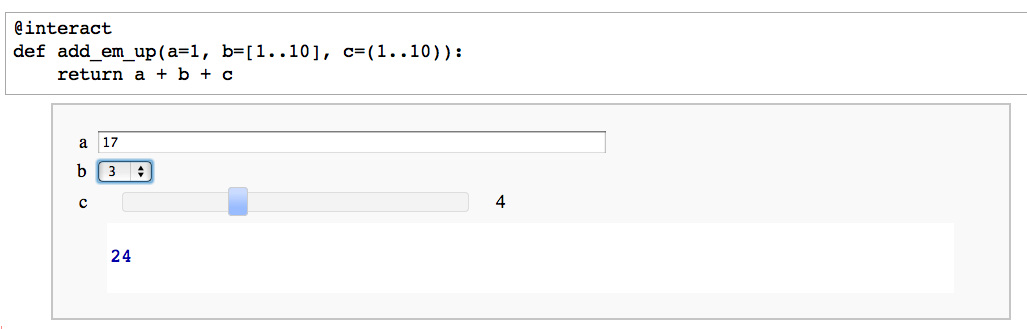
\includegraphics[width=.5\textwidth]{graphics/interact}
\end{center}

A hope you can {\em sense the possibilities...}.  Here we do type checking:

%skip
\begin{lstlisting}
class returns:
    def __init__(self, typ):
        self._typ = typ
    def __call__(self, f):
        return lambda *args, **kwds: self._typ(f(*args, **kwds))


@returns(float)
def f(n,m):
    """Returns n + m."""
    return n + m
\end{lstlisting}
Let's try it out:
%skip
\begin{lstlisting}
sage: f(2,3)
5.0
sage: type(f(5,6))
<type 'float'>
sage: f('4', '123')
4123.0
\end{lstlisting}

Here's another example I use all the time.  If you put {\tt
  @parallel(ncpus)} before a function {\em and} you call the function
using a list as input, then the function gets evaluated at each
element of the list in parallel, and the results are returned as an
iterator.  If you call the function without giving a list as input, it
just works as usual (not in parallel).


%skip
\begin{lstlisting}
@parallel(10)
def f(n):
    sleep(1)   # make function seem slow
    return n*(n+1)/2
\end{lstlisting}
First, try it not in parallel, which takes a long time. 
%skip
\begin{lstlisting}
%time
sage: for n in [1..10]: print n, f(n)
1 1
2 3
3 6
4 10
5 15
6 21
7 28
8 36
9 45
10 55
CPU time: 0.00 s,  Wall time: 10.00 s
\end{lstlisting}

Now try it in parallel:
%skip
\begin{lstlisting}
%time
sage: for X in f([1..10]): print X
(((1,), {}), 1)
(((2,), {}), 3)
(((3,), {}), 6)
(((4,), {}), 10)
(((5,), {}), 15)
(((6,), {}), 21)
(((7,), {}), 28)
(((8,), {}), 36)
(((9,), {}), 45)
(((10,), {}), 55)
CPU time: 0.19 s,  Wall time: 1.32 s
\end{lstlisting}



\section{The Ecosystem}

The Sage distributuion itself consists of about 100 open source
programs and libraries, which (like Linux) are developed by a loosely
knit international group of programmers.  Many of these programs are
written as Python libraries.

Any software engineer knows that a programming language is much more
than just the formal language specification or even a particular
implementation.  It's also the user community, the general pace of
development, and---most importantly---the collections of tools and
libraries that are available in that language, especially the free
ones.  Python excels in available tools, as the following list of many
of the Python-based components of Sage attests:

\begin{itemize}
\item Pycrypto -- fast implementations of many cryptosystems.
\item Cython -- a Python compiler and tool for efficient use of C/C++
  libraries from Python.  We will have much more to say about Cython
  in Chapter~\ref{ch:cython}.
\item IPython -- interactive interpreter shell
\item Jinja2 -- HTML and other templating tools; popular for web
  applications.
\item Moinmoin -- a standalone wiki, e.g., the one used by \url{http://wiki.sagemath.org}.
\item PIL -- Python imaging library (a ``programmable Photoshop'')
\item Pygments -- HTML source code highlighting
\item SQLalchemy -- abstracts interface to most SQL databases and an
  object:relational mapper.
\item Sphinx -- ReST documentation system for Python, which is used by
  many Python projects (including Sage).
\item Twisted -- a networking framework; everything from web applications
      to email to ssh servers are implemented in Twisted.
\item ZODB -- The Zope object-oriented database
\item arpack -- A sparse numerical linear algebra library.
 \item CVXopt -- A library for solving convex (and other) optimization problems. 
 \item Docutils -- related to Python documentation 
 \item easy-install -- you can do \verb|easy_install foobar| to
   install any of the over 13,000 Python packages available at
   \url{http://pypi.python.org/}.

\item gd -- very quickly draw png images with lines, arcs, etc.

 \item matplotlib -- the canonical Python 2d graphics library

 \item mpmath -- arbitrary precision floating point mathematics
   special functions, numerical integration, matrices, etc.

 \item NumPy -- an $n$-dimensional array library, which is the
   fundamental package needed for scientific computing with Python.

 \item pexpect -- control command-line subprocesses

 \item rpy2 -- fast compiled interface to the R statistics program,
   which is also included in Sage.

 \item sage -- the Sage library; mainly implements mathematical
   algorithms, especially symbolic ones.

 \item sagenb -- the Sage notebook web application (can be used
   standalone separate from Sage).

 \item sagetex -- allows you to embed Sage in \LaTeX{} documents

 \item SciPy -- a large library of numerical functions that are useful
   in mathematics, science, and engineering, including numerical
   integration, optimization, statistics, differential equations, etc.

\item setuptools -- package for distributing and working with standalone python packages

 \item SymPy -- a lightweight Python library for symbolic mathematics.
 \end{itemize}

\section{Exercise: Build Python from Source}
If your computer operating system is Linux or OS X (with XCode
installed), it is an easy ``exercise'' to build the Python language
from source.  This is particularly relevant if you want to understand
Python more deeply, since you can change anything you want in the
interpreter itself, recompile, and try out the result!

First, go to \url{http://python.org/download/} and download some
version of Python.  I am using OS X (with XCode installed) and choose
Python 3.2.   In a few seconds I have the file 
{\tt Python-3.2.tar.bz2} in my {\sf Downloads} folder.
Using the {\sf Terminal} application, I navigate to that folder, extract
Python, configure and build it, which takes under 2 minutes (!).
%skip
\begin{lstlisting}
deep:~ wstein$ cd Downloads
deep:Downloads wstein$ tar xf Python-3.2.tar.bz2 
deep:Downloads wstein$ cd Python-3.2
deep:Python-3.2 wstein$ ./configure; time make -j8
...
real	1m18.284s
user	1m59.552s
sys	0m9.980s
deep:Python-3.2 wstein$
\end{lstlisting}

And now let's try it out:
\begin{lstlisting}
deep:Python-3.2 wstein$ ./python.exe 
Python 3.2 (r32:88445, Mar 30 2011, 10:20:45) 
[GCC 4.2.1 (Apple Inc. build 5666) (dot 3)] on darwin
Type "help", "copyright", "credits" or "license" for more 
information.
>>> 2 + 2
4
\end{lstlisting}

For fun, let's change something in the core of Python, recompile, and
observe our change.  On line 288 of {\tt
  Python-3.2/Objects/listobject.c}, I insert a line that calls the C
{\sf printf} function to print out some graffiti:
\begin{lstlisting}
...
PyObject *
PyList_GetItem(PyObject *op, Py_ssize_t i)
{ 
    printf("Hi Mom!\n");           /* I added this! */
    if (!PyList_Check(op)) {
        PyErr_BadInternalCall();
...
\end{lstlisting}

I then type {\tt make} again, wait a few seconds, and try out Python again:
\begin{lstlisting}
deep:Python-3.2 wstein$ ./python.exe 
Python 3.2 (r32:88445, Mar 30 2011, 10:25:56) 
[GCC 4.2.1 (Apple Inc. build 5666) (dot 3)] on darwin
Type "help", "copyright", "credits" or "license" for more 
information.
Hi Mom!
...
Hi Mom!
>>> v = [1,2,3]
>>> v[0]
1
>>> v['a']
Traceback (most recent call last):
  File "<stdin>", line 1, in <module>
Hi Mom!
Hi Mom!
Hi Mom!
Hi Mom!
Hi Mom!
TypeError: list indices must be integers, not str
\end{lstlisting}

Interestingly, the function \verb|PyList_GetItem| appears to not be
called when we use an integer to access a list, but it is used when we
try to access the list with anything else.

For more information about how the Python source code is laid out,
see the README file, especially the section at the end called
``Distribution structure''.

\chapter{Cython}\label{ch:cython} 

In addition to the Sage-related examples and discussion below, to
really learn Cython, I strongly recommend that you read straight as
much of the Cython Users Guide (see
\url{http://docs.cython.org/src/userguide/}) as you can trying out
everything, and the other Cython documentation (see
\url{http://docs.cython.org/}) as well.

\section{An Example: Speeding up a Simple Function}

Let's start with a first simple example.  We write a Python program
that computes the sum of the integers up to $n$ using a naive
bruteforce algorithm\footnote{Of course, a better approach is to use
  the formula $\sum_{i=1}^n = \frac{n(n+1)}{2}$!}
%skip
\begin{lstlisting}
def python_sum(n):
    # Python int's are faster than Sage ints for very small numbers
    s = int(0)    
    for i in range(1, n+1):
        s += i
    return s
\end{lstlisting}

Now try it out:
%skip
\begin{lstlisting}
sage: python_sum(10^5)
5000050000
sage: timeit('k = python_sum(10^5)')
25 loops, best of 3: 11.9 ms per loop
\end{lstlisting}

Let's rewrite this program, but in Cython (which is a Pythonish-to-C
compiler).  Note that our ``rewritten'' program looks identical---the
only difference so far is that we told Sage to compile the program
using Cython by putting {\tt \%cython} at the beginning of the block
(If you are using the command line instead of the notebook, put the
code without \verb|%cython|
in a file \verb|foo.pyx|, then type \verb|load foo.pyx|.)

%skip
\begin{lstlisting}
%cython
def cython_sum(n):
    s = int(0)
    for i in range(1, n+1):
        s += i
    return s
\end{lstlisting}

If you evaluate the above code in the Sage notebook, you'll see that
two linked files appear after the input cell:
\begin{enumerate}
\item A file that ends in .c: this is the C program that the above
  code got turned into.  This is compiled and linked automatically
  into the running copy of Sage.
\item A file that ends in .html: this is an annotated version of the
  above Cython program; double click on a line to see
  the corresponding C code.
\end{enumerate}

Is the Cython program any faster?
%skip
\begin{lstlisting}
sage: cython_sum(10^5)
5000050000
sage: timeit('cython_sum(10^5)')      # your mileage may vary
25 loops, best of 3: 12.1 ms per loop
\end{lstlisting}

What?! If you were to think very carefully about what the computer is
actually doing when running \verb|cython_sum| and \verb|python_sum|,
you would find that it is doing the same thing in both cases.  In
the case of \verb|python_sum|, the Python interpreter is carrying out a
sequence of operations (calling functions in the Python C library),
and in the case of \verb|cython_sum|, a C program is running (the
compiled Cython module), which is simply calling exactly the same
functions in the Python C library.  

To get a major speedup, we must {\em change the game}.  Cython makes
this possible by letting you declare variables to have a specific
datatype.  When you understand the implications of this (do not worry
if you don't yet!), you can safely write code that in some situations
is dramatically faster, depending on the situation.  Observe:

%skip
\begin{lstlisting}
%cython
def cython_sum_typed(n):
    cdef long i, s
    s = 0
    for i in range(1, n+1):
        s += i
    return s
\end{lstlisting}
The {\em only} difference is that we added a single new line:
\verb|cdef long i, s|.  This tells Cython to treat {\tt i} and {\tt s}
as being of data type {\tt long}, which is a 32 or 64-bit integer,
depending on the computer you're using.  This is literally the same as
the long datatype in C/C++/Java.


%skip
\begin{lstlisting}
sage: cython_sum_typed(10^5)
5000050000
sage: timeit('cython_sum_typed(10^5)')
625 loops, best of 3: 69.4 µs per loop
sage: 11.9/.069
172.463768115942
\end{lstlisting}
By adding that one line  we made our code over 170
times faster!


But watch out, {\tt long} integers silently {\em overflow}, and
silently behave differently depending on whether you're using a 32 or
64-bit operating system.  It is absolutely critical to understand this
distinction if you want to make truly effective use of computers.

The following example illustrates overflow:
%skip
\begin{lstlisting}
%cython
def longmul(long a, long b): 
    return a*b
\end{lstlisting}
Now let's try it:

%skip
\begin{lstlisting}
sage: longmul(2^10, 2^20)
1073741824
sage: longmul(2^20, 2^50)   # overflows!
0
sage: 2^20 * 2^50
1180591620717411303424
\end{lstlisting}


\section{Using External C/C++ Code}

Cython is absolutely critical to the design of Sage, and potentially
very important to your own work, because it makes it possible to
efficiently make use of data types and functions defined in any C/C++
library.  Since there is an enormous amount of useful, fast, debugged
C/C++ code out there, Cython gives your Sage and Python programs
access to vast amounts of useful capabilities.  Also, when used
correctly, there is no overhead in calling out to the C libraries,
unlike the situation with SWIG, ctypes, and many other approaches
to writing C library wrappers.

\subsection{Simple random example}
Here's a first simple example.  Type {\tt man random} on the command line
(or Google it) to find out about the random C library function:
\begin{lstlisting}
RANDOM(3)                BSD Library Functions Manual  RANDOM(3)

NAME
     initstate, random, setstate, srandom, srandomdev -- better 
     random number generator; routines for changing generators

LIBRARY
     Standard C Library (libc, -lc)

SYNOPSIS
     #include <stdlib.h>

     char *
     initstate(unsigned seed, char *state, size_t size);

     long
     random(void);
...
\end{lstlisting}

Despite {\tt random} being a function defined in the standard C
library, we can still call it from Cython, as follows:
%skip
\begin{lstlisting}
%cython
cdef extern from "stdlib.h":                  # (1) 
    long random()                             # (2)

def random_nums(int n):                       # (3)
    cdef int i                                # (4)
    v = [random() for i in range(n)]          # (5)
    return v
\end{lstlisting}

Let's try it out:
%skip
\begin{lstlisting}
sage: random_nums(5)
[1315705257, 1147455227, 1571270137, 1106977565, 1805149207]
sage: timeit('v = random_nums(10^5)')
125 loops, best of 3: 5.56 ms per loop
\end{lstlisting}

It's interesting to see how this compares to pure Python.  Here's the same program in Python:
%skip
\begin{lstlisting}
%python
import random
k = 2**31-1
def py_random_nums(n):
    return [random.randint(0,k) for i in range(n)]
\end{lstlisting}
So the speedup is by a factor of nearly 50:
%skip
\begin{lstlisting}
sage: py_random_nums(5)
[317567506, 1289482476, 1766134327, 1216261810, 1427493671]
sage: timeit('v = random_nums(10^5)')
5 loops, best of 3: 251 ms per loop
sage: 251/5.56
45.1438848920863
\end{lstlisting}

Finally we explain the above code line by line. (TODO)



\subsection{Adding rational numbers using MPIR}

We next consider a more mathematical example: arithmetic with
arbitrary precision rational numbers.  The MPIR C library (which is
included with Sage, but can also be downloaded separately for free for
any standard operating system from \url{http://mpir.org/}) provides
highly optimized arithmetic with arbitrary precision integers and
rational numbers.\footnote{MPIR and GMP \url{http://gmplib.org/} are
  basically the same for our discussion; technically they are
  ``forks'' of each other, but export essentially the same functions.}
We could make use of MPIR by reading the documentation for MPIR and
using {\tt cdef extern} as above.  Fortunately, all of the necessary
{\tt cdef extern} declarations needed to use MPIR are already declared
in Sage.  You can view all the declarations from the notebook by
navigating to {\tt <url of notebook server>/src/libs/gmp}.

Let's use MPIR directly to create two rational numbers and add them
together.  The code below is complicated and illustrates many issues
and techniques, so we will explain it in great depth.  Once you
understand this, you can deal with many issues that will come up with
Cython.

%skip
\begin{lstlisting}
%cython
from sage.libs.gmp.all cimport *                      # (1)          
def add_rationals(bytes a, bytes b):                  # (2)
    cdef mpq_t x, y, z                                # (3)
    mpq_init(x); mpq_init(y); mpq_init(z)             # (4)
    mpq_set_str(x, a, 10)    # base 10 string         # (5)
    mpq_set_str(y, b, 10)                             
    mpq_add(z, x, y)                                  # (6)
    cdef int n = (mpz_sizeinbase (mpq_numref(z), 10)  # (7)
          + mpz_sizeinbase (mpq_denref(z), 10) + 3)
    cdef char* s = <char*>sage_malloc(sizeof(char)*n) # (8)
    if not s: raise MemoryError                       # (9)
    cdef bytes c = mpq_get_str(s, 10, z)              # (10)
    mpq_clear(x); mpq_clear(y); mpq_clear(z)          # (11)
    sage_free(s)                                      # (12)
    return c
\end{lstlisting}

Now let's try it out:
%skip
\begin{lstlisting}
sage: add_rationals('2/3', '-5/21')
'3/7'
sage: 2/3 - 5/21
3/7
sage: add_rationals('1/29048203984092834823049', 
           '-394/29302938402384092834')
'-11444963066794174536188472/851197732045760533660225724673976778930866'
\end{lstlisting}

Timings suggest we didn't mess up:
%skip
\begin{lstlisting}
sage: timeit("add_rationals('2/3', '-5/21')")
625 loops, best of 3: 1.29 µs per loop
sage: timeit('2/3 - 5/21')
625 loops, best of 3: 2.16 µs per loop
\end{lstlisting}
Here's a simplistic check that we probably didn't screw up and
introduce any memory leaks. (Go up to the code and comment out some
frees to see how this changes.)

%skip
\begin{lstlisting}
sage: print get_memory_usage()
sage: timeit("add_rationals('9012038409238411/13', 
              '-4/9082309482309487')",number=10^6)
sage: get_memory_usage()
917.5625
1000000 loops, best of 3: 1.72 µs per loop
917.5625
\end{lstlisting}

Finally, we will go line by line through the code and explain exactly
what is going on and why. TODO


\section{Important Cython Language Constructions}
In this section we systematically go through {\em the most important}
standard Cython language constructions.  We will not talk about using
numpy from Cython, dynamic memory allocation, or subtleties of the C
language in this section.  Instead we cover declaring and using cdef'd
variables, explicit type casts, declaring external data types and
functions, defining new Cython cdef'd functions, and declaring new
Cython cdef'd classes that can have C attributes. 

\subsection{Declaring Cython Variables Using {\tt cdef}}
\begin{lstlisting}
cdef type_name variable_name1, variable_name2, ...
\end{lstlisting}
The single most important statement that Cython adds to Python is
\begin{lstlisting}
cdef type_name
\end{lstlisting}
This allows you to declare a variable to have a type.  The possibilities for the type include:
\begin{itemize}
\item C data type: int, float, double, char.  Each can be modified by: short, long, signed, unsigned. 
\item Certain Python types, including: list, dict, str, object (=Python object), etc. 
\item Name of a known {\tt cdef class} (see below).  You may have to cimport the class.
\item More complicated C/C++ data types: struct, C++ class, typedef, etc., that have been declared using some other method described below.
\end{itemize}

\begin{lstlisting}
%cython
def C_type_example():
    # ^ = exclusive or -- no preparsering in Cython!
    cdef int n=5/3, x=2^3   
    cdef long int m=908230948239489394
    cdef float y=4.5969
    cdef double z=2.13
    cdef char c='c'
    cdef char* s="a C string"
    print n, x, m, y, z, c, s
\end{lstlisting}
When we run the above function, we get the following.  Note the lack
of preparsing, and that the char variable {\tt c} is treated as a
number.
\begin{lstlisting}
sage: C_type_example()
1 1 908230948239489394 4.59689998627 2.13 99 a C string
\end{lstlisting}

\begin{lstlisting}
%cython
def type_example2(x, y):
    cdef list v
    cdef dict z
    v = x
    z = y
\end{lstlisting}
  
\begin{lstlisting}
sage: type_example2([1,2], {'a':5})
sage: type_example2(17, {'a':5})
Traceback (most recent call last):
...
TypeError: Expected list, got sage.rings.integer.Integer
sage: type_example2([1,2], 17)
Traceback (most recent call last):
...
TypeError: Expected dict, got sage.rings.integer.Integer
\end{lstlisting}

For the Cython source code of Sage integers, in the Sage library see
\verb|rings/integer.pxd| and \verb|rings/integer.pyx|.  Also, browse
\verb|libs/gmp/| for the definition of functions such as
\verb|mpz_set| below.

\begin{lstlisting}
%cython
from sage.rings.integer cimport Integer   # note the cimport!
def unsafe_mutate(Integer n, Integer m):
    mpz_set(n.value, m.value)
\end{lstlisting}

\begin{lstlisting}
sage: n = 15
sage: print n, id(n)
15 54852752
sage: unsafe_mutate(n, 2011)
sage: print n, id(n)
2011 54852752
\end{lstlisting}


\subsection{Explicit casts}
\begin{lstlisting}
    <data_type> foo
\end{lstlisting}

If you need to force the compiler to treat a variable of one data type
as another, you have to use an explicit cast.  In Java and C/C++ you
would use parenthesis around a type name, as follows:

\begin{lstlisting}
int i = 1;
long j = 3;
i = (int)j;
\end{lstlisting}

In Cython, you use angle brackets (note: in Cython this particular
cast isn't strictly necessary to get the code to compile, but in Java
it is):

\begin{lstlisting}
%cython
cdef int i = 1
cdef long j = 3
i = <int> j
print i
\end{lstlisting}

Here's an example where we convert a Python string to a char* (i.e., a
pointer to an array of characters), then change one of the characters,
thus mutating an immutable string.

\begin{lstlisting}
%cython
def unsafe_mutate_str(bytes s, n, c):
    cdef char* t = <char*>s
    t[n] = ord(c)
\end{lstlisting}
Try it out:
\begin{lstlisting}
sage: s = 'This is an immutable string.'
sage: print s, id(s), hash(s)
This is an immutable string. 72268152 -5654925717092887818
sage: unsafe_mutate_str(s, 9, ' ')
sage: unsafe_mutate_str(s, 11, ' ')
sage: unsafe_mutate_str(s, 12, ' ')
print s, id(s), hash(s)
This is a    mutable string. 72268152 -5654925717092887818
sage: hash('This is a    mutable string.')
-7476166060485806082
\end{lstlisting}

\subsection{Declaring External Data Types and Functions}

In order for Cython to make use of a function or data type defined in
external C/C++ library, Cython has to {\em explicitly} be told what
the input and output types are for that function and what the function
should be called.  Cython will then generate appropriate C/C++ code
and conversions based on these assumptions.  There are a large number
of files in Sage and Cython itself that declare all the functions
provided by various standard libraries, but sometimes you want to make
use of a function defined elsewhere, e.g., in your own C/C++ library,
so you have to declare things yourself.  The purpose of the following
examples is to illustrate how to do this.  It is also extremely useful
to look at the Sage library source code for thousands of additional
nontrivial working examples.
\begin{lstlisting}
cdef extern from "filename.h":
     declarations ...    
\end{lstlisting}

The following examples illustrates several different possible
declarations.  We'll describe each line in detail.  This first example
declares a single type of round function on doubles -- it's as
straightforward as it gets.
\begin{lstlisting}
%cython
cdef extern from "math.h":
    double round(double)

def f(double n):
    return round(n)    
\end{lstlisting}
Try it out:
\begin{lstlisting}
sage: f(10.53595)
11.0
\end{lstlisting}

Now suppose we want a version of round that returns a long. By
consulting the man page for round, we find that there is a round
function declared as follows:
\begin{lstlisting}
    long int lround(double x);
\end{lstlisting}
We can declare it exactly like the above, or we can use a C ``name
specifier'', which let's us tell Cython we want to call the function
{\tt round} in our Cython code, but when Cython generates code it should
actually emit {\tt lround}.  This is what we do below.

\begin{lstlisting}
%cython
cdef extern from "math.h":
    long int round "lround"(double)

def f(double n):
    return round(n)    
\end{lstlisting}

\begin{lstlisting}
sage: f(10.53595)
11
\end{lstlisting}

Another case when using C name specifiers is useful if you want to be
able to call both a C library version of a function and a builtin
Python function with the same name.

\begin{lstlisting}
%cython
cdef extern from "stdlib.h":
    int c_abs "abs"(int i)
 
def myabs(n):
    print abs(n)
    print c_abs(n)    
\end{lstlisting}
Now use it:
\begin{lstlisting}  
sage: myabs(-10)
10
10
\end{lstlisting}

We can also declare data types and variables using {\tt cdef extern}.
To write the code below, I used the {\tt man} command on my computer
several times on each referenced function.  I knew the relevant
functions because I read a book on the C programming language when I
was a freshman; learning the basics of the C programming language and
standard libraries is a very good idea if you want to be able to make
effective use of Cython... or computers in general, since most systems
programming is done in C.

Coming up with the declarations below is a little bit of an art form,
in that they are not exactly what is given from the man pages, though
they are close.  Just realize that the declarations you give here do
exactly one thing: they inform Cython about what C code it should
generate, e.g., it will convert the string {\tt "w"} below to a {\tt
  char*} before calling the {\tt fopen} function.  That's it, that's
all the declarations do; they do not have to be perfect.  You should
evaluate this code in the notebook and click on the .html file that is
produced, then look at the corresponding C code, to see what I mean.

\begin{lstlisting}
%cython
cdef extern from "stdio.h":
    # We use void* since we don't care about structure of FILE
    ctypedef void* FILE   
    FILE* fopen(char* filename, char* mode)
    int fclose(FILE *stream)
    int fprintf(FILE *stream, char *format, ...)
    
def f(filename):
    cdef FILE* file
    file = fopen(filename, "w")
    fprintf(file, "Hi Mom!")
    fclose(file)
\end{lstlisting}

Let's try create create and write to a file using the above code:
\begin{lstlisting}
sage: f('foo.txt')
sage: print open('foo.txt').read()
Hi Mom!
\end{lstlisting}

It's unlikely you would ever want to access the above functions from
Cython, since they are already nicely wrapped by Python itself.
Nontheless, if you need total control and speed when doing file
access, you have it.

\subsection{Defining New Cython Functions}
In addition to using the {\tt cdef} keyword to define variables as
above, we can also define functions.  These are like Python functions,
but you can declare the input types and the return type explicitly,
and calling them is then blazingly fast, as compared to calling
regular Python functions.  (Remember, most of the point of Cython is
speed, speed, speed! The other point of Cython is that you can call
C/C++ functions from Cython; that is less relevant if you don't care
about speed, because there is something else called ctypes that allows
you to do that directly from Python.)

\begin{lstlisting}
cdef return_type function_name(type1 input1, type2 input2...):
    # body of function
\end{lstlisting}

Here is an example, where we create both a cdef and regular function
to add two int's.  Note that the return type of the cdef function can
itself by a C data type, but the same is not true for the return type
of a Python function.  We will see below that the cdef function is
dramatically faster, since there is very little overhead in calling
it.  
\begin{lstlisting}
%cython
cdef int add_cython(int a, int b):
    return a + b
        
def add_python(int a, int b):
    return a + b    

def f(int n):
    cdef int i, s=0
    for i in range(n):
        s += add_cython(s, i)                          
    return s    

def g(int n):
    cdef int i, s=0
    for i in range(n):
        s += add_python(s, i)                               
    return s    
\end{lstlisting}

Let's test it:
\begin{lstlisting}
sage: timeit('f(10^6)')
625 loops, best of 3: 595 µs per loop
sage: timeit('g(10^6)')
5 loops, best of 3: 94.6 ms per loop
sage: 94.6/.595
158.991596638655
\end{lstlisting}
Indeed, we find that the cdef'd function is 159 times faster!

Notice that \verb|add_python| is callable from the interpreter, but
\verb|add_cython| isn't:
\begin{lstlisting}
sage: add_python(2,8)
10
sage: add_cython(2,8)
Traceback (most recent call last):
...
NameError: name 'add_cython' is not defined
\end{lstlisting}

The {\tt cpdef} keyword lets us define a function that is somewhere intermediate
between a Python function and a cdef'd function.
If we use {\tt cpdef} instead of {\tt cdef} then everything is almost
identical, except the {\tt cpdef}'d method can also be called from Python.
This is often mainly useful for testing and general usability.  The
{\tt cpdef} method will be slightly slower though.  In this example, it is
about 4 times slower. 
\begin{lstlisting}
cpdef return_type function_name(type1 input1, type2 input2...):
    # function body
\end{lstlisting}

Here is the example:
\begin{lstlisting}  
%cython

cpdef int add_cython2(int a, int b):
    return a + b
        
def f2(int n):
    cdef int i, s=0
    for i in range(n):
        s += add_cython2(s, i)                          
    return s      
\end{lstlisting}
Now test it out:
\begin{lstlisting}  
sage: timeit('f2(10^6)')
125 loops, best of 3: 2.63 ms per loop
sage: 2.63/.595
4.42016806722689
sage: add_cython2(2,8)   # the function is available
10
\end{lstlisting}

\subsection{Defining New Cython Classes}

One of the most powerful features of Cython is that you can define new
classes that have C-level attributes and cdef'd methods.  The cdef'd
attributed and function calls are very, very fast to use.  

\begin{lstlisting}
cdef class ClassName(base_class):  
     cdef type_name variable
     # ...
     # Then functions mostly like a Python class, except 
     # you can include cdef'd methods with input and output
     # types as in the previous section.  
     # ...
     # There are some subtleties with special methods such
     # as __add__ and __hash__; see the Cython documentation.
\end{lstlisting}
   
Note that cdef'd classes in Cython can have at most one base class;
there is no support for multiple inheritance.  This is a basic design
decision with Cython, and is very unlikely to ever change.  You can of
course create non-cdef'd classes in Cython that have multiple
inheritance.

Here is an example in which we create a Cython class that wraps a
Python string, and provides the ability of changing the entries of the
string:

\begin{lstlisting}
%cython
cdef class StringMutator:
    cdef bytes s    # cdef's attribute    
    def __init__(self, bytes s):
        self.s = s        
    def __setitem__(self, int i, bytes a):
        if i < 0 or i >= len(self.s): raise IndexError
        if len(a) != 1: raise ValueError
        (<char*> self.s)[i] = (<char*>a)[0]
    def __repr__(self): return self.s    
    def __str__(self): return "%s"%self.s
\end{lstlisting}

\begin{lstlisting}
sage: s = "Hello World"
sage: t = StringMutator(s)
sage: t[4] = 'X'
sage: print s
HellX World
sage: print t
HellX World
\end{lstlisting}

Notice that setting an entry is fast:
\begin{lstlisting}
sage: timeit("t[4]='X'", number=10^5)
100000 loops, best of 3: 226 ns per loop
\end{lstlisting}
We did include some bounds checking to avoid crashes:
\begin{lstlisting}
sage: t[100] = 'x'
Traceback (most recent call last):
...
IndexError
\end{lstlisting}
We can also convert from mutable string back and get a new string:
\begin{lstlisting}
sage: m = str(t); m
'HellX World'
sage: t[0] = 'X'; t
XellX World
sage: m
'HellX World'
\end{lstlisting}


\section{Numpy and Cython}

\begin{verbatim}
<h1 style="text-align: center;">Lecture 12: Numpy + Cython = AWESOME</h1>
<p>This lecture is about how to efficiently combine Numpy and Cython to write fast numerical code.</p>
<p>We will focus on the problem of computing the <em>standard deviation</em>&nbsp;of a list of floating point numbers. &nbsp; Let $x_1, \ldots, x_n$ be a list of $n$ real numbers, and let $$\mu = \frac{1}{n}\sum_{i=1}^n x_i$$ be their mean. &nbsp; We define their standard deviation to be $$\sqrt{\frac{1}{n}\sum_{i=1}^n (x_i - \mu)^2}.$$</p>
<p><strong>Note</strong>: In statistics it is common to divide by $n-1$ instead of $n$ when computing the standard deviation of a sample and using it to estimate the standard deviation of a population. &nbsp;We will not do this, since our goal today is illustrating programming techniques, not learning techniques of statistics.</p>
<p>&nbsp;</p>
<p><strong>Running Example:</strong> Compute the standard deviation of a list of 64-bit floating point numbers. &nbsp; Our data set is computed using the random.random method, which generates numbers <strong>uniformly</strong> between 0 and 1.</p>

{{{id=3|
set_random_seed(0)
import random
v = [random.random() for _ in range(10^5)]
///
}}}

{{{id=84|
v[:20]
///
[0.43811732887872634, 0.78344784289564662, 0.7917672531341533, 0.43546157784257289, 0.99879630143646858, 0.21470214570255253, 0.52818002353940696, 0.51667692205628102, 0.67726646422202585, 0.92183464863760212, 0.54553592061123968, 0.2143866131543859, 0.90130600825854523, 0.71144055233831971, 0.080614713472959898, 0.81024524942438758, 0.8403186842969067, 0.26527690630696821, 0.9755892062984004, 0.94353224947123771]
}}}

<p>First we write a naive straightforward implementation of computation of the standard deviation.</p>

{{{id=9|
def my_std(z):
    mean = sum(z)/len(z)
    return sqrt(sum((x-mean)^2 for x in z)/len(z))
///
}}}

{{{id=10|
time my_std(v)
///
0.28871143425255896
Time: CPU 0.06 s, Wall: 0.06 s
}}}

{{{id=11|
timeit('my_std(v)', number=10)
///
10 loops, best of 3: 64.8 ms per loop
}}}

<p>Next we try the std function in Sage, which was implemented by UW undergrad Andrew Hou as part of paid work he did on Sage after he took Math 480.</p>

{{{id=1|
time std(v, bias=True)
///
0.28871143425255896
Time: CPU 0.03 s, Wall: 0.03 s
}}}

{{{id=12|
timeit('std(v, bias=True)')
///
25 loops, best of 3: 26.4 ms per loop
}}}

<p>Next we try Numpy, which is much faster than the above.</p>

{{{id=7|
import numpy
v_numpy = numpy.array(v, dtype=numpy.float64)
///
}}}

{{{id=14|
v_numpy.dtype
///
dtype('float64')
}}}

{{{id=21|
v_numpy.std()
///
0.28871143425255896
}}}

{{{id=6|
timeit('v_numpy.std()')
///
625 loops, best of 3: 1.25 ms per loop
}}}

{{{id=76|
22.5/1.25
///
18.0000000000000
}}}

<p>Sage also has code for working with TimeSeries, which happens to have a method for computing the standard deviation. &nbsp;It is a couple of times faster than Numpy. &nbsp;</p>

{{{id=16|
v_stats = stats.TimeSeries(v)
///
}}}

{{{id=85|
v_stats.variance??
///
}}}

{{{id=20|
v_stats.standard_deviation(bias=True)
///
0.28871143425255896
}}}

{{{id=15|
timeit('v_stats.standard_deviation(bias=True)')
///
625 loops, best of 3: 240 µs per loop
}}}

<p>The TimeSeries code is nearly optimal. &nbsp;A TimeSeries is represented by a contiguous array of double's, and the code for computing standard deviation is very straightforward Cython that maps directly to C. &nbsp;(I wrote it, by the way.)</p>

{{{id=17|
1.25/.236
///
5.29661016949153
}}}

<p><strong>Goal: </strong>Write a function that computes the standard deviation of a numpy array as quickly as stats.TimeSeries does, hence is faster than Numpy itself.</p>
<p>First approach: Use numpy "vectorized operations". &nbsp;This doesn't help at all (and is also wasteful of memory, by the way).</p>

{{{id=86|
def std_numpy1_oneline(v):
    return math.sqrt(((v - v.mean())**2).mean())
///
}}}

{{{id=23|
def std_numpy1(v):
    m = v.mean()  # mean of entries
    w = v - m     # subtracts m from each entry: "broadcasting"
    w2 = w**2     # squares each entry componentwise. 
    return math.sqrt(w2.mean())
///
}}}

{{{id=88|
get_memory_usage()
///
864.90625
}}}

{{{id=89|
w = v_numpy**2
///
}}}

{{{id=90|
get_memory_usage()
///
865.671875
}}}

{{{id=19|
std_numpy1(v_numpy)
///
0.28871143425255896
}}}

{{{id=87|
std_numpy1_oneline(v_numpy)
///
0.28871143425255896
}}}

{{{id=18|
timeit('std_numpy1(v_numpy)')
///
625 loops, best of 3: 1.25 ms per loop
}}}

<p>Let's see how the time gets spent between each step. &nbsp;It turns out to be about equally spent among each line.</p>

{{{id=34|
m = v_numpy.mean()
timeit('v_numpy.mean()')
///
625 loops, best of 3: 140 µs per loop
}}}

{{{id=37|
w = v_numpy - m
timeit('v_numpy - m')
///
625 loops, best of 3: 241 µs per loop
}}}

{{{id=38|
w2 = w**2
timeit('w**2')
///
625 loops, best of 3: 157 µs per loop
}}}

{{{id=36|
m2 = w2.mean()
timeit('math.sqrt(w2.mean())')
///
625 loops, best of 3: 143 µs per loop
}}}

{{{id=91|
sqrt(2)
///
sqrt(2)
}}}

{{{id=92|
math.sqrt(2)
///
1.4142135623730951
}}}

{{{id=93|
a = float(2)
timeit('sqrt(a)', number=10^5)
///
100000 loops, best of 3: 589 ns per loop
}}}

{{{id=94|
timeit('math.sqrt(a)', number=10^5)
///
100000 loops, best of 3: 216 ns per loop
}}}

{{{id=39|

///
}}}

<p>Next try Cython with no special type declarations. &nbsp;Not surprisingly, this does not help in the least bit.</p>

{{{id=28|
%cython

import math
def std_numpy2(v):
    m = v.mean()  # mean of entries
    w = v - m     # subtracts m from each entry: "broadcasting"
    w2 = w**2     # squares each entry componentwise. 
    return math.sqrt(w2.mean())
///
}}}

{{{id=25|
std_numpy2(v_numpy)
///
0.28871143425255896
}}}

{{{id=24|
timeit('std_numpy2(v_numpy)')
///
625 loops, best of 3: 1.3 ms per loop
}}}

<p>Next try Cython with special support for Numpy. &nbsp;This gets powerful... as we will see.</p>

{{{id=30|
%cython

from numpy cimport ndarray
import math
def std_numpy3(ndarray v not None):
    m = v.mean()  # mean of entries
    w = v - m     # subtracts m from each entry: "broadcasting"
    w2 = w**2     # squares each entry componentwise. 
    return math.sqrt(w2.mean())
///
}}}

{{{id=96|
std_numpy3(None)
///
Traceback (most recent call last):
  File "<stdin>", line 1, in <module>
  File "_sage_input_68.py", line 10, in <module>
    exec compile(u'open("___code___.py","w").write("# -*- coding: utf-8 -*-\\n" + _support_.preparse_worksheet_cell(base64.b64decode("c3RkX251bXB5MyhOb25lKQ=="),globals())+"\\n"); execfile(os.path.abspath("___code___.py"))' + '\n', '', 'single')
  File "", line 1, in <module>
    
  File "/tmp/tmpXdvvgn/___code___.py", line 2, in <module>
    exec compile(u'std_numpy3(None)' + '\n', '', 'single')
  File "", line 1, in <module>
    
  File "_sagenb_flask_sage_notebook_sagenb_home_openidSfmMv1OuVE_44_code_sage70_spyx_0.pyx", line 8, in _sagenb_flask_sage_notebook_sagenb_home_openidSfmMv1OuVE_44_code_sage70_spyx_0.std_numpy3 (_sagenb_flask_sage_notebook_sagenb_home_openidSfmMv1OuVE_44_code_sage70_spyx_0.c:713)
    def std_numpy3(ndarray v not None):
TypeError: Argument 'v' has incorrect type (expected numpy.ndarray, got NoneType)
}}}

{{{id=33|
std_numpy3(v_numpy)
///
0.28871143425255896
}}}

{{{id=42|
timeit('std_numpy3(v_numpy)')
///
625 loops, best of 3: 1.7 ms per loop
}}}

<p>Look at Cython + Numpy documentation (by Googling "cython numpy"), and we learn that if we declare v a little more precisely, then we get fast direct access to the underlying elements in v.</p>

{{{id=46|
%cython

cimport numpy as alex
import math

def std_numpy4a(alex.ndarray[alex.float64_t, ndim=1] v not None):
    cdef Py_ssize_t i
    cdef Py_ssize_t n = v.shape[0]   # how many entries
    
    # Compute the mean
    cdef double m # = 0
    for i in range(n):
        m += v[i]    
    m /= n
    # just doing the mean for now...
    return m
///
}}}

{{{id=45|
std_numpy4a(v_numpy)
///
0.49896857465357608
}}}

<p>Timing looks good...</p>

{{{id=44|
timeit('std_numpy4a(v_numpy)')
///
625 loops, best of 3: 376 µs per loop
}}}

{{{id=79|

///
}}}

<p>Let's finish it the function and see how it compares.</p>

{{{id=56|
%cython

cimport numpy as np
cdef extern:
    double sqrt(double)

def std_numpy4b(np.ndarray[np.float64_t, ndim=1] v):
    cdef Py_ssize_t i
    cdef Py_ssize_t n = v.shape[0]   # how many entries
    
    # Compute the mean
    cdef double m = 0
    for i in range(n):
        m += v[i]    
    m /= n
    
    # Compute variance
    cdef double s = 0
    for i in range(n):
        s += (v[i] - m)**2
    
    return sqrt(s/n)
///
}}}

{{{id=55|
std_numpy4b(v_numpy)
///
0.28871143425255896
}}}

{{{id=63|
timeit('std_numpy4b(v_numpy)')
///
625 loops, best of 3: 274 µs per loop
}}}

{{{id=54|
timeit('v_stats.standard_deviation(bias=True)')
///
625 loops, best of 3: 238 µs per loop
}}}

{{{id=58|
timeit('v_numpy.std()')
///
625 loops, best of 3: 1.27 ms per loop
}}}

<p>Very nice!!</p>

{{{id=60|

///
}}}

<p>Finally, we try again, after disabling bounds checking. &nbsp; This is even better; almost as good as stats.TimeSeries.</p>

{{{id=50|
%cython

cimport numpy as np
cdef extern:
    double sqrt(double)
    
# turn of bounds-checking for entire function    
cimport cython
@cython.boundscheck(False) 
def std_numpy5a(np.ndarray[np.float64_t, ndim=1] v):
    cdef Py_ssize_t i
    cdef Py_ssize_t n = v.shape[0]   # how many entries
    # Compute the mean
    cdef double m = 0
    for i in range(n):
        m += v[i]    
    m /= n
    # Compute variance
    cdef double s = 0
    for i in range(n):
        s += (v[i] - m)**2
    return sqrt(s/n)
///
}}}

{{{id=49|
timeit('std_numpy5a(v_numpy)')
///
625 loops, best of 3: 227 µs per loop
}}}

{{{id=43|
timeit('v_stats.standard_deviation(bias=True)')
///
625 loops, best of 3: 240 µs per loop
}}}

<h1><span style="color: #800000;">Yeah, we did it!! &nbsp;</span>&nbsp;</h1>
<p>For smaller input, interestingly we get a massive win over Numpy. &nbsp; If you were, e.g., computing a sliding window of standard deviations (say) for a time series, this would be important.</p>

{{{id=65|
a = numpy.array([1,2,3,4], dtype=float); a
///
array([ 1.,  2.,  3.,  4.])
}}}

{{{id=67|
timeit('std_numpy5a(a)')
///
625 loops, best of 3: 483 ns per loop
}}}

{{{id=68|
timeit('a.std()')
///
625 loops, best of 3: 24.4 µs per loop
}}}

{{{id=69|
b = stats.TimeSeries(a)
timeit('b.standard_deviation(bias=True)')
///
625 loops, best of 3: 534 ns per loop
}}}
\end{verbatim}

\chapter{Resources for Solving Problems Using Sage}

\section{The Sage Library}

You can do a Google search on all of the Sage documentation, web pages
and discussion groups all in one go by visiting the webpage
\url{http://sagemath.org/search.html} and typing in your search, then
waiting as the page dynamically updates.

Of course you can find links to the standard Sage documentation, including
the tutorial, constructions guide, FAQ, developer's guide, and reference manual
at \url{http://sagemath.org/help.html}.  There are also links to videos and
many other helpful materials there.      

There are numerous quick reference cards at
\url{http://wiki.sagemath.org/quickref} which list numerous Sage
commands on a single page in specific areas such as Calculus and
Linear Algebra.  Much work went into creating these cards, and they
are an excellent resource to print out.

If you want to search the documentation of the functions defined in
the Sage library, use the \verb|search_doc| command.  This just does a
straight search through all the docstrings of the functions in the
HTML version of the Sage documentation, without any prebuilt index.
It is written in Python and uses regularly expressions on the source
code to extract docstrings out and find your search terms.  The
\verb|search_doc| command works on both the command line and in the
notebook.  On the command line it displays one line from each HTML
document, so is tedious to actually use.  In the notebook, it displays
the relevant html documents, which links to each.  If you click on a
link, you'll go to an interactive version of the relevant section of
the documentation, where you can search that page for relevant text.
Watch out, since stupidly you then have to use the back button to get
back to your worksheet -- it would be better if the html output of
\verb|search_doc| used \verb|<a target="_new" href="...">|; until this is
changed, you may want to right click and select "open in new tab".
\begin{lstlisting}
sage: search_doc('eigenvalue')
...
\end{lstlisting}

The HTML documentation for Sage is far from complete; there is lots of
code in the Sage library that isn't documented at all in the HTML
documentation of Sage, for whatever reason.   You can easily search through
all of this code by typing \verb|search_src(...)| on either the
command line or in the notebook. 
\begin{lstlisting}
sage: search_src('eigenvalue')
...
\end{lstlisting}
On the command line you'll get a list of each line in each file that
contains the given search term.  In the notebook, you will get a list
of all files in the Sage library that contain the search term, along
with links to the files.  The same caveats regarding clicking on the
links applies as with \verb|search_doc| (see above).  When you click
on a file, it will look funny for a moment (a bug, in my opinion),
then suddenly refresh and display as a very nicely formated and syntax
highlighted page. You should then search this page for your term, in
order to see it in context.  At the top of the page there is also a
link called ``browse directory'', which lets you browse to any file in
the Sage library and similarly view it. 

To search the definitions of function, use \verb|search_def|.  This works
just like \verb|search_src| but restricts the search to the definition
lines of functions.
\begin{lstlisting}
sage: search_def('other_graph')
...
\end{lstlisting}


\section{Question and Answer Sites}

The Sage project hosts their own question and answer site devoted to
Sage at \url{http://ask.sagemath.org}.  You can instantly sign in
using OpenID and ask a question, or answer one.  Specific answerable
questions are best.  You can also easily search all the questions, and
see if anybody has asked a similar question before (and what the
answers were).  The answers are ranked based on user voting, and the
questions are sorted by tags.  People are motivated to give good answers,
since they get ``karma points'' for posting useful answers.

One of the first big question/answer sites is
\url{http://stackoverflow.com/}, which has a huge number of questions
and answers about all things related to coding. One of the top most
popular tags is ``python'', with over 50000 question.  There are also
a few dozen questions taged ``sage'' (some about the Sage math
software, and some about the unrelated Sage accounting software).  If
you run into Python programming questions, this can be an excellent
site on which to search for answers or ask questions.

\section{Documentation for components of Sage}
There are many components of Sage that offer vast amounts of
functionality, and have excellent documentation, but you'll find
almost nothing about them in any of the standard Sage documentation.  
For example, for numerical computing numpy, scipy, and cvxopt are
all included in Sage, and often many, many capabilities that are
well documented in their respected documentation.  Thus it is
quite useful to know that you can do the following:
%listing
\begin{lstlisting}
sage: import scipy.special
sage: scipy.special.<call some function>
\end{lstlisting}

There is a list of all packages included in every recent copy of Sage
at \url{http://sagemath.org/packages/standard/}.  

Usually the best way to find the documentation for one of these
optional components of Sage is to use Google.  Search for the
component by name and possibly throw in a word like ``math'' or if it
the component is a Python library the word ``python''.  For example,
there is a component of Sage called {\tt mpmath}, and you can find its
website by doing a google search for... {\tt mpmath}.  Once there, it
is easy to find the documentation, and you should quickly be able to
start using mpmath's functionality from within Sage.

If you have your own Sage install, you can also install nearly any
Python library you want into it. However, this is not an easy option
if you're using a public Sage notebook server that somebody else
administers.

\section{Live Chat}

There is a live IRC chatroom where you can ask for help anytime, and
maybe get some feedback.  All you have to do is point your webbrowser
to \url{http://sagemath.org/help-irc.html}, fill in the form, and
you're chatting.  Type {\tt /who} to see a list of people logged into
the forum.  

\chapter{Sage Development}

\section{Overview of Sage Development}

{\bf Motivating Problem:} {\em Suppose you want to modify or improve Sage
in some way, and want your changes to be included in a future release
of Sage. How do you do this?}

\subsection{What is a Sage Release?}
New versions of Sage are released about once every month or two, so it
is possible for your contribution to get into Sage and start being
used by people relatively quickly.  A new release of Sage consists of
both an updated version of the code in the Sage library, and updated
versions of some of the roughly 90 third-party packages that Sage
includes.  Before each release, this code (over 6 million lines) is
all built from source on dozens of hardware/OS combinations, and
hundreds of thousands of tests are run to increase the chances Sage
will actually work correctly when you use it.

The way in which Sage is distributed---as both a core library and its
dependencies---is highly unusual in the world of open source software,
though it is similar to how other mathematical software of comparable
size and scope to Sage is released (Magma, Mathematica, Matlab, Maple,
Enthought's Python Distribution, etc.)  Mathematical software is
highly interrelated and extremely sensitive to even the slightest
changes anywhere in the system, and because Sage has such a large test
suite, we notice these issues.  It is a constant and difficult battle
just to keep the components of Sage working together as new and
hopefully improved releases of each component appear.

Each new Sage release has an associated changelog, which lists all of
the changes that were made to Sage in that release, along with
everybody who contributed to the release.  You can find a list of
these at \url{http://sagemath.org/mirror/src/changelogs/}



The changelog for Sage-4.6.2 looks like this:
%skip
\begin{lstlisting}
Sage 4.6.2 was released on 28 February 2011. It is available at
           http://www.sagemath.org/download.html
  * About Sage (http://www.sagemath.org)
...
The following 100 people contributed to this release. Of those, 25 
made their first contribution to Sage:

  * Alain Filbois [first contribution]
  * Alain Giorgetti [first contribution]
  * Alexandre Blondin Massé
  * Alexey U. Gudchenko [first contribution]
  * Alex Ghitza
  * Aly Deines
  ...
  * William Stein
  * Wolfgang Steiner [first contribution]
  * Yann Laigle-Chapuy
  * Yann Ponty [first contribution]

* Release manager: Jeroen Demeyer.

* Doctesting coverage:

  * Overall weighted coverage score:  84.8%  (84.4% for 4.6.1)
  * Total number of functions:        27200  (26816 for 4.6.1)

* We closed 221 tickets in this release. For details, see

  http://sage.math.washington.edu/home/release/sage-4.6.2/tickets.html

Closed tickets:

 #116: notebook doctest -- should be able to doctest a worksheet, 
       so we can distribute worksheets with SAGE [Reviewed by 
       Willem Jan Palenstijn]
#5389: Creating a  updated GAP workspace with -tp is racy 
       [Reviewed by Willem Jan Palenstijn]
#8216: Make David Perkinson's sandpile 2.2 module an experimental 
       (at least) package [Reviewed by David Kirkby]
#9641: Race condition with sage -tp [Reviewed by Willem Jan 
       Palenstijn]
#9809: Graph.num_edges() gives wrong answer [Reviewed by Minh 
       Van Nguyen]
...
#10816: Volker Braun: Subscheme creation does not work from the 
       notebook [Reviewed by Jeroen Demeyer]
#10842: Jeroen Demeyer: Increase timeouts in sage/tests/cmdline.py 
       [Reviewed by Volker Braun]
\end{lstlisting}


Notice that 100 (!) different people contributed improvements and bug fixes to Sage-4.6.2, 
which was a release that took just over a month to appear. 
Of these, 25 were first-time contributors.

There were 221 ``trac tickets'' closed in this release.  Each ticket
description is listed after a number.  Visit
\url{http://sage.math.washington.edu/home/release/sage-4.6.2/tickets.html}
for an easy-to-navigate list of these tickets, which links to
\url{http://trac.sagemath.org}, or search for {\tt \#number} in the
search box in the upper right.

For example, consider ticket \#10336.  This ticket is an
``enhancement'', not a bug fix, that includes a code submission by
{\tt novoselt}, a.k.a. Andrew Novoseltsov, who is a Russian graduate
student studying algebraic geometry in Canada (who used to be a Univ.
of Washington graduate student).  When you view the ticket you'll see
how long ago the patch was posted, that little improvements were made,
and that {\tt vbraun}, a.k.a. Volker Braun (a Physicist in Ireland)
gives the work a positive review.  Moreover, two months after the
first code was submitted, it was merged into sage-4.6.2.alpha2 by {\tt
  jdemeyer}, who is a Belgium number theorist.

Notice that before a final Sage release is made there are a sequence
of alpha releases, e.g., sage-4.6.1.alpha1, sage-4.6.1.alpha2, and
also release candidates.  It is important to emphasize that these are
all completely public releases, which anybody can try out, and the
source code for all of them, including in progress releases, is
available at \url{http://sage.math.washington.edu/home/release/}.
There are other open source projects, even components of
Sage\footnote{For example, GAP \url{http://www.gap-system.org/}.}),
that keep their alpha releases secret or semisecret; we believe this
is a counterproductive approach to the creation of open source
software, and that it is best to keep every step of the development
process open.

\subsection{Hurdles}
There are several hurdles to getting your code into Sage:
\begin{itemize}

\item You have to use the {\em command line}.  It is currently simply
  not possible to use only the notebook for Sage development... yet!

  \item  You have to know {\em basic UNIX} commands: ls, cp, cd, mv, etc.

  \item  You have to have some understanding of {\em the Sage Python library} and our 
       coding conventions and requirements.

  \item You have to submit {\em patches} to the trac webpage, which
       requires using the Mercurial distributed revision control
       system.  Thus you must become familiar with the basic use of a
       distributed revision control system. This is good for you anyways. 

     \item All patches go through a {\em peer review} process, just
       like a formally published paper.  Somebody has to referee your
       work, signing off on it publicly, before your work can go into
       Sage.  Beyond testing whether the code works and is stylish,
       this process also includes asking whether it makes sense to
       include your code in Sage at all; we usually do not want
       third-rate code.
\end{itemize}


Fortunately, the process is well documented (see
\url{http://sagemath.org/doc/developer/}), there are thousands of
examples of tickets along with the complete review process
at \url{http://trac.sagemath.org}, and there are numerous
Sage Days workshops that help people get up to speed. Around five
hundred people have successfully got code into Sage, and you can too
if you are serious.

\subsection{Walkthrough}

We will do a careful slow step-by-step live demo that illustrates some
of Sage development.
%skip
\begin{lstlisting}
<pre>my_laptop ssh math480@sage.math.washington.edu

math480@sage:~$ cd scratch
math480@sage:~/scratch$ ls
sage-4.6.2-sage.math.washington.edu-x86_64-Linux.tar.gz
math480@sage:~/scratch$ mkdir wstein
math480@sage:~/scratch$ cd wstein/
math480@sage:~/scratch/wstein$ ls
math480@sage:~/scratch/wstein$ tar xf ../sage-4.6.2-sage.math.washington.edu-x86_64-Linux.tar.gz 
[[Wait about 1 minute.]]
math480@sage:~/scratch/wstein$ mv sage-4.6.2-sage.math.washington.edu-x86_64-Linux sage
math480@sage:~/scratch/wstein$ cd sage/
math480@sage:~/scratch/wstein/sage$ ls
COPYING.txt  devel     ipython	Makefile    sage		 spkg
data	     examples  local	README.txt  sage-README-osx.txt  VERSION.txt
math480@sage:~/scratch/wstein/sage$ here  # sets up path
math480@sage:~/scratch/wstein/sage$ sage
----------------------------------------------------------------------
| Sage Version 4.6.2, Release Date: 2011-02-25                       |
| Type notebook() for the GUI, and license() for information.        |
----------------------------------------------------------------------
The Sage install tree may have moved
...
Done resetting paths
sage: 2 + 3
5
\end{lstlisting}

Now make some change (using vim, emacs, pico, etc.), do "sage -br" to
make change take effect.  Then make a patch and export it.

\section{How to modify the Sage library and create a patch}
\begin{verbatim}
     0. Turn on screen capture using Quicktime (plus I'll do this all in one terminal and paste the session log below, though editing won't get recorded).
     1. Login to the math480@sage.math.washington.edu account.  NOTE: On Windows, install [http://www.chiark.greenend.org.uk/~sgtatham/putty/ Putty]. On Linux and OS X use the command line (e.g., Terminal) and type "ssh math480@sage.math.washington.edu". 
     2. Change to directory with my sage install in it and type "here" to setup PATH.
     2. Make a change to the Sage library source code using pico, based on a suggestion from class.
     3. Save the change and test it using "sage -br"
     4. Type "hg diff" to see the change (your shell current working directory must be a subdirectory of SAGE_ROOT/devel/sage/)
     5. Type "hg commit" to save changes as a commit.  Type "hg revert --all" to instead undo everything you have done.  Enter a log message on the first line and save the file, when you do "hg commit".
     6. Type "hg log|more" to see that you have done something.
     7. Type "hg export tip > file.patch" to create a patch file.   You can get the patch by navigating to the directory in which you typed this command, starting here: http://sage.math.washington.edu/home/math480/scratch/
     8. Congrats, we have our patch.   If we don't like it and want to start over, do "hg rollback".  This will reset things to be exactly like they were before we typed "hg commit" above. 
     9. Remark: For much finer control over making patches, people usually use "Mercurial Queues", as described here in [http://sagemath.org/doc/developer/ The Sage developers guide].      You do not have to use them for your homework. 
\end{verbatim}

%%%%%%%%%%%%%%%%%%%%%%%%%%%%%%%%%%%%%%%%%%%%%%%%%%%%%%%%%%%%%%%%
\chapter{How Sage Uses Other Math Software Systems}\label{ch:interfaces}

\begin{verbatim}
<p>The goal of this lecture is to give you a deeper understanding of some of the fundamental and unique architectural issues involved in Sage.</p>
<p>I built Sage partly from other complete mathematical software systems because I wanted to finish Sage (for my use!) in at most 5 years.&nbsp;</p>
<h3 style="text-align: center;">"Building the car instead of reinventing the wheel."</h3>
<p>Some of the major components included in Sage are:</p>
<ul>
<li>PARI/GP - number theory</li>
<li>GAP - group theory</li>
<li>Singular - commutative algebra</li>
<li>Maxima - symbolic calculus</li>
<li>R - statistics</li>
</ul>
<p>Each of the above is a full standalone project with its own custom programming language, history, culture, etc. &nbsp;And each has unique, powerful, debugged code that I don't want to have to rewrite from scratch, since it would take too long, and writing code from scratch is incredibly difficult and frustrating.&nbsp;</p>
<p>I also wanted to make it easy to call the following systems from Sage for the purposes of benchmarking, porting, migration of users and code, optional functionality, etc.:</p>
<ul>
<li>Magma</li>
<li>Maple</li>
<li>Mathematica</li>
<li>Mupad</li>
<li>Matlab</li>
<li>Axiom, Octave, REDUCE, Macaulay2, Scilab, Kash, Lisp</li>
</ul>
<p>&nbsp;</p>
<p><strong>The Big Problem:</strong> How can we make use of the above systems from Python?</p>
<p>This question is difficult partly because there are so many answers, each with pros and cons, and I had to choose (then be criticized for my choices).</p>
<p>&nbsp;</p>
<p>&nbsp;</p>
sage: number_of_partitions(10)
42
sage: list(Partitions(10))
[[10], [9, 1], [8, 2], [8, 1, 1], [7, 3], [7, 2, 1], [7, 1, 1, 1], [6, 4], [6, 3, 1], [6, 2, 2], [6, 2, 1, 1], [6, 1, 1, 1, 1], [5, 5], [5, 4, 1], [5, 3, 2], [5, 3, 1, 1], [5, 2, 2, 1], [5, 2, 1, 1, 1], [5, 1, 1, 1, 1, 1], [4, 4, 2], [4, 4, 1, 1], [4, 3, 3], [4, 3, 2, 1], [4, 3, 1, 1, 1], [4, 2, 2, 2], [4, 2, 2, 1, 1], [4, 2, 1, 1, 1, 1], [4, 1, 1, 1, 1, 1, 1], [3, 3, 3, 1], [3, 3, 2, 2], [3, 3, 2, 1, 1], [3, 3, 1, 1, 1, 1], [3, 2, 2, 2, 1], [3, 2, 2, 1, 1, 1], [3, 2, 1, 1, 1, 1, 1], [3, 1, 1, 1, 1, 1, 1, 1], [2, 2, 2, 2, 2], [2, 2, 2, 2, 1, 1], [2, 2, 2, 1, 1, 1, 1], [2, 2, 1, 1, 1, 1, 1, 1], [2, 1, 1, 1, 1, 1, 1, 1, 1], [1, 1, 1, 1, 1, 1, 1, 1, 1, 1]]
sage: time number_of_partitions(10^7)
92027175502604546685596278166825605430729405281023979395328576351741298526232350197882291654710333933219876431112892669442996519201446933718057425885425510196566971369272243936886123704944390011846626724222935883880949646021554674211449712293631879438242092222979701858787035045131791561718499094276679781015502944193307504577212918898104161448934354538420643899518683659226259312517022343012768006249066347774384224200200491423135789948628712467862610060006610227873354093344771970346402912468019502617741296485750068965727678736574879683519236357061319134860914524427627076446580477740857594944050855144756641881148963046419111504530928013165254773178279374714115048498031936743061146399094602347281946619566715867818368113040887581799683872172944577575391666322871295451048112070492385908727524159239222366587691028630013147462129464573569940173628469758175515190001641345140899367093190859080267185611792170429465197857968117435299141079155705662249617336911859509285578584413441733816964914269258918743530174261522145886491433067881470395832647408578195566042566460494284912372612048505127243987254597660690323804252237148083121685300106473794690689801747504661946299472005981442948094926764563853171727831538610914056742150737497538427502124024964209080033657278768694168219946346309906686670220404292685540282106667661584147201155740243521818020629234011924167214100674819982674459329845176126920689181532303574746823885977198276651255478126323692431978852519785180336170541394768609366389114772406136683349412746708709224596935940110215929918473383014389065632764805267657590865513593978244244311680854217735536592823219001199569770431572718888108452817614295777255622715362408122265800848932276196267545354426556723347685735897551768373108977390874033016418618266068861412680046926417299574367992118065543824471964711585682146618651730116890773279227432137954488457335074000412015820488115033194548391813526724286716271750346470118187739995800431441608729698516332428256345862484406623639956273335472545741134762782834725659303362718667415197368798040219223371637134331256426629887430519590196027703231191899072357523708159719377437782971846471928181434133277347743728346062720786947891744911516248998265758156411629802345973249527007535170095624359891373084013345497111826508558570667664488643633183476426421938705419176750248730025527079093923132020478303851642054200888831310378483811088425548758508373324093873479730273437693679342081086702018520971877967092726990888474755041255077282275352308667980953624552474645295774554823817830271752015905175487656200680986962732503598211618667111264793583287147032328796244469851598884862190118775508811358918545701650113647140734902415801399931326365622784208807398682277421689531141855076998289838068746126554377321750652288128533274971246389513818051037817849704769088911818484659276794986806465634286299339344423718490667472287384981129496643999747556606122301402027411096367172771385437211572122448922846957076711812454645572143320128971630906382167345381586565940316748316082706877584540948496188398233399350019423833682423300814059493159013417591894979385650634324308841947277121816559279335938926911510683549043290690287102733571315222761846482615431786061813454633634415974179413942024706129986725734471552346167738613509470760758338637870579921007168514417341548481513953296373455058614174692678013759737246724696931125240457406888289154055030387593548942880549262383621259594080699698643245355453826567378500963781681659096276126857969078217677288980
Time: CPU 0.32 s, Wall: 0.32 s
<p><strong>Problem 1:</strong> Availability of a specific known version of a third party software package.</p>
<p>Even if we solve the big problem above, a "vendor" will often just release a new version of their software with numerous changes that break our solution. &nbsp;This happens <em>constantly</em>. &nbsp;And the actual versions of software that people have installed (under OS X, various Linuxes, Solaris, etc.) will be widely distributed over versions of software from the last decade. &nbsp; &nbsp;</p>
<p><strong>Solution: </strong>For the free open systems that (1) we really need, and (2) we can build from source easily enough, we ship and build a very specific version as part of Sage. &nbsp; This completely solves problem 1, at the expense of a lot of (misplaced) criticism from people who don't understand the problem; at the same time, this accidentally creates a solution to a different problem (easy-to-install distribution of a bunch of useful math software), which many people greatly appreciate.&nbsp;</p>
<p>For the non-free systems or the free systems that are hard to build, the problem just doesn't get solved. &nbsp;And indeed our interfaces and code that relies on those systems is sadly fairly brittle; often a new version of Magma just breaks with Sage. &nbsp; Fortunately, of course very little functionality in Sage depends on such systems.&nbsp;</p>
<p>&nbsp;</p>
<p>&nbsp;</p>
<p><strong>Problem 2</strong>: Make a specific version of some mathematics software (call it M) usable from Python.</p>
<p>Here are some of the many potential approaches to this problem:</p>
<ol>
<li><strong>Naive Subprocess. </strong>Start up M, tell it to read in a file, and save the results in a file, and terminate. &nbsp;<em>This doesn't preserve state between calls, and startup time can easily be seconds, so this is not viable.</em></li>
<li><strong>Create network protocols.</strong> &nbsp;Define an openmath/XML based protocol for well-defined communication of "arbitrary mathematics" (whatever that is) between software, e.g., between M and Python. &nbsp;Design and implement client and server protocols. &nbsp;<a href="http://www.symbolic-computation.org/The_SCIEnce_Project" target="_blank">The SCIEnce project</a>, started in 2006, and costing many millions of dollars, is an example. &nbsp; <em>This seems like the right approach, but it it is slow in certain relevant benchmarks and too challenging (for me) to develop. &nbsp;It's probably very useful for something (e.g., writing research papers), but is massively too complicated for what we need for Sage, which is focused on what is practical now.</em></li>
<li><strong>Pseudo-tty's (ptty) = pexpect. </strong>&nbsp; Create a simulated command line prompt that is controled by Python. &nbsp;Absolutely anything that one can do at the command line with M immediately becomes usable from a Python program. &nbsp; &nbsp;This is relatively easy to implement and extremely flexible -- one can create a useful interface to any math software system out there in a day. &nbsp;It is slow in some sense, but still much better than (1) and (2). &nbsp; <em>This approach has been used in Sage for a long time.</em></li>
<li><strong>C/C++ library interfaces.</strong> &nbsp;Create a C/C++ library interface and link the other program into Python itself, using Cython. &nbsp; This is extremely difficult, because none of the M's (except PARI) are designed to be used this way. &nbsp;However, it is extremely fast. &nbsp;For basic arithmetic, it can be several hundred times faster than (3) above. &nbsp;</li>
</ol>
<p>As of now, people have written fairly polished versions of both (3) and (4) for all of: PARI, GAP, Singular, Maxima, and R. &nbsp; &nbsp;In case of (4), these are all hard work, and aren't necessarily used much in Sage yet, or even included in Sage, but they exist, and are on the way in.&nbsp;</p>
<p>The rest of this worksheet is about how to use (3) above: the pexpect based interfaces. &nbsp; This is <em>well worth learning</em>, because these interface all work in almost exactly the same way, and there are interfaces to pretty much every math software system out there. &nbsp; Sage is the only software in existence that can talk to so many other math software systems. &nbsp;</p>
<p>Here are the basic points, which we'll follow with several examples illustrating them. &nbsp;Suppose m is one of math software systems, e.g., r or singular or maxima:</p>
<ul>
<li><strong>x = m.eval(s): </strong>sets x equal to the string obtained by typing the string s into M. &nbsp; The string s can be several lines long. &nbsp;(This is how many % modes in the noteboook are implemented.)</li>
<li><strong>x = m(s): </strong>creates a new Python object that "wraps" the result of evaluating s in M. &nbsp;It's like typing "x.name() = s" into M. &nbsp;You can then do arithmetic with x, and call functions on it, e.g., <strong>x.function(...)</strong> or <strong>m.function(..., x, ...)</strong>.&nbsp;</li>
</ul>
<p>And that is pretty much it. &nbsp;</p>
<p><strong>WARNING:</strong> There is latency. &nbsp;<strong>Any</strong> time you call any function involving a pexpect interface, expect it to take on the order of at least <strong>1ms (=one millisecond), </strong>even if the actual operation in the system M takes almost no time. &nbsp; &nbsp;For comparison, adding or multiplying most simple objects in Python/Sage takes about 1 microsecond (i.e., 1/1000 the time of a call involving pexpect), and adding/multiping objects in Cython can take only a few nanoseconds (1/1000000 the time of a pexpect call). &nbsp;</p>
sage: %lisp
sage: (* 5 7)
35
sage: lisp.eval('(* 5 7)')
'35'
sage: %maxima
sage: a:5
sage: b:7
sage: a*b
5
7
35
<h2>Examples</h2>
<p>Another note: the very first time you do m.eval(...) it may take surprisingly long, since another program is starting up.</p>

<p>We use Maxima to illustrate evaluation of a simple string:</p>
sage: s = maxima.eval("2 + 3")
sage: type(s)
<type 'str'>
sage: s
'5'
sage: maxima.eval("""
...      a : 2;
...      b : 3;
...      c : a +b;
...
sage: """)   
sage: maxima.eval('c')
'5'
sage: timeit('maxima.eval("2+2")')
625 loops, best of 3: 1.2 ms per loop
sage: a = maxima('2')
sage: timeit('a + a')
625 loops, best of 3: 1.37 ms per loop
sage: timeit('2+2')
625 loops, best of 3: 331 ns per loop
<p>There is now a separate Maxima subprocess running. &nbsp;Each process has an id number associated to it:</p>
sage: maxima.pid()   # the "pin id" of the subprocess
9259
<p>Next will illustrate creating a Python object that wraps an expression in Maxima.</p>
sage: s = maxima('sin(x^3) * tan(y)')
sage: type(s)
<class 'sage.interfaces.maxima.MaximaElement'>
sage: float(1.31*10^(-3) / (330*10^(-9)))
3969.69696969697
<p>The name of the object in the corresponding Maxima session:</p>
sage: s.name()
'sage2656'
<p>The object prints nicely:</p>
sage: s
sin(x^3)*tan(y)
<p>Latex output happens to be supported:</p>
sage: show(s)
<html><div class="math">\newcommand{\Bold}[1]{\mathbf{#1}}\sin x^3\,\tan y</div></html>
sage: maxima.eval('sage2656 + 1')
'sin(x^3)*tan(y)+1'
<p>You can call functions on objects in a Pythonic way.</p>
sage: s.integrate('y')
sin(x^3)*log(sec(y))
<p>Or use maxima.function(...)</p>
sage: maxima.integrate(s, 'y')
sin(x^3)*log(sec(y))
<p>The result is another Python object (which wraps another object defined in Maxima). &nbsp;We can call functions on that object as well.</p>
sage: z = s.integrate('y')
sage: type(z)
<class 'sage.interfaces.maxima.MaximaElement'>
sage: z
sin(x^3)*log(sec(y))
sage: z.name()
'sage2662'
sage: z.diff('y')
sin(x^3)*tan(y)
sage: z + z
2*sin(x^3)*log(sec(y))
<p><strong>Conclusion:</strong> If you understand the above, you are in extremely good shape. &nbsp;All the other interfaces work the same way. &nbsp; The examples below are just to illustrate some subtle points and show how interfaces are useful. &nbsp;</p>
sage: z.jksadhflksd()
jksadhflksd(sin(x^3)*log(sec(y)))
sage: z_sage = z.sage(); z_sage
log(sec(y))*sin(x^3)
sage: type(z_sage)
<type 'sage.symbolic.expression.Expression'>
sage: maxima(z_sage)
sin(x^3)*log(sec(y))
<p>It is possible in some systems to seriously mess things up and get things "out of sync". &nbsp;This is nearly impossible with Maxima, since we use it so heavily and have debugged the heck out of it. &nbsp;However, with other systems (like Magma) this can happen. &nbsp;If it does, do, e.g., <strong>maxima.quit()</strong>. &nbsp;This completely kills the subprocess, invalides any Python objects that wrap variables in that session, and starts a brand new fresh session. &nbsp;</p>
<p>Here is an example with each of the five big systems included in Sage:</p>
sage: maxima('2+3')  # maxima
5
sage: gp('2+3')  # pari/gp
5
sage: singular('2+3')
5
sage: gap('2+3')
5
sage: r('2 + 3')
[1] 5
sage: z_sage._maxima_init_()
'(log(sec(y)))*(sin((x)^(3)))'
<p>You can follow standard R tutorials and have the computations (except graphics at present) to all definitely "just work". &nbsp;(Unlike the potentially confusing rpy2.)&nbsp;</p>
sage: x = r('c(1,3,2,10,5)');  y = r('1:5')
sage: print x
sage: print y
[1]  1  3  2 10  5
[1] 1 2 3 4 5
sage: x + y
[1]  2  5  5 14 10
sage: x/y
[1] 1.0000000 1.5000000 0.6666667 2.5000000 1.0000000
sage: x.length()
[1] 5
sage: x > 3
[1] FALSE FALSE FALSE  TRUE  TRUE
sage: x[x > 3]
[1] 10  5
<p>There is also an interface to Octave, which is very similar to Matlab (but free).</p>
sage: A = octave('rand(3)'); A
 0.401446 0.286955 0.396858
 0.606625 0.371021 0.515619
 0.96863 0.683554 0.837288
sage: A*A
 0.719642 0.492938 0.639562
 0.968042 0.664185 0.863772
 1.61454 1.1039 1.43791
sage: A.rref()
 1 0 0
 0 1 0
 0 0 1
<p><strong>Bonus:</strong> There is even a pexpect interface to Sage itself. &nbsp; (Trivia: this is used in the implementation of the Sage notebook.)</p>
sage: sage0('2 + 3')
5
sage: A = sage0('matrix(QQ, 3, [1..9])'); A
[1 2 3]
[4 5 6]
[7 8 9]
sage: type(A)
<class 'sage.interfaces.sage0.SageElement'>
sage: A.echelon_form()
[ 1  0 -1]
[ 0  1  2]
[ 0  0  0]
<p>Let's get crazy: a pexpect interface inside a pexpect interface. &nbsp;And of course, this code is going from the notebook to Sage via yet another interface.</p>
sage: sage0.eval('sage0 = Sage()')
sage: z = sage0('sage0("3+5")')
sage: type(z)
<class 'sage.interfaces.sage0.SageElement'>
sage: z
8
sage: sage0.type(z)
<class 'sage.interfaces.sage0.SageElement'>
\end{verbatim}



%%%%%%%%%%%%%%%%%%%%%%%%%%%%%%%%%%%%%%%%%%%%%%%%%%%%%%%%%%%%%%%%
\part{Using Sage}

\chapter{Graphics}

\section{2d Plots}

\begin{verbatim}
<p>Sage has plotting support that covers:</p>
<ul>
<li>most 2d plotting that Mathematica has (with a similar interface)</li>
<li>3d plotting, somewhat like Mathematica</li>
<li>most 2d plotting that Matlab has (with a similar interface)</li>
</ul>
<p>Sage uses the Python library Matplotlib (<a href="http://matplotlib.sourceforge.net/" target="_blank">http://matplotlib.sourceforge.net/</a>) is used under the hood to render 2d graphics; for 3d graphics, Sage can use a Java applet (jmol), an HTML5 canvas renderer, or a raytracer. &nbsp;</p>
<p>In this worksheet, we'll explain how to use the "mathematica-style" 2d plotting capabilities of Sage.</p>
<h1>Drawing Lines</h1>
<p>First, we'll discuss a simple but very powerful plotting command in Sage called "line". &nbsp;It takes as input a list of points, and draws a sequence of line segments connecting them. &nbsp; &nbsp;The points are given as 2-tuples (x,y), which are the x and y coordinates of a point in the plane. &nbsp; The output of calling the line command is a line object. &nbsp;</p>
sage: L = line([(-2,-2), (3,8), (5, 5)])
sage: print L
Graphics object consisting of 1 graphics primitive
<p>To <em><strong>see</strong></em> the actual plot of L, just put L by itself on a line or type show(L) or L.show():</p>
sage: L
<html><font color='black'><img src='cell://sage0.png'></font></html>
sage: show(L)
<html><font color='black'><img src='cell://sage0.png'></font></html>
sage: L.show()
<html><font color='black'><img src='cell://sage0.png'></font></html>
<p>Incidentally, there are many, many options that you can pass to the show command. &nbsp; The three most useful are:</p>
<ul>
<li>frame=True: &nbsp; Make it so the x-y axis are replaced by a frame, which is much better when looking at certain types of plots</li>
<li>gridlines=True: Adds a background grid, which makes it easier to understand the plot in some cases.</li>
<li>figsize=[w,h]: &nbsp;Allows you to adjust the size of the output. &nbsp;Think of w and h as the width and height in "inches".&nbsp;</li>
</ul>
<p>You can combine these options. &nbsp;For example:</p>
sage: L.show(frame=True, gridlines=True, figsize=[8,2])
<html><font color='black'><img src='cell://sage0.png'></font></html>
<p>&nbsp;In the notebook you can just click and download the default plots displayed above, since they are png images. &nbsp; However, if you want to include images in a paper you're writing, or use an image in an editor such as Inkscape, it's much better to save the images in other formats. &nbsp; Thus a&nbsp;critically useful command is L.save('filename.ext'), which enables you to save a graphics object to a file. &nbsp;The extension of the filename determines the type of the file. &nbsp;For example, below we save L to pdf, eps, and svg formats. &nbsp;Note that the svg image just appears embedded in your web browser, and you can pan around. &nbsp;In any case, you can always (right or control) click on the link or image to save it as a file on your computer. &nbsp; &nbsp;&nbsp;</p>
sage: L.save('image.pdf')
sage: L.save('image.eps')
sage: L.save('image.svg')
<p>Lines (and all other graphics objects) have numerous properties that you can adjust, which you find in the documentation. &nbsp;The most important properties of lines are:</p>
<ul>
<li>color=...: where for the color you can give a string, e.g., 'red'; or an html color, e.g., '#042a99', or an rgb triple.</li>
<li>thickness=4: &nbsp;the thickness of the line</li>
<li>linestyle='--': &nbsp; the style of the line: '--', '-.', '-', ':'</li>
</ul>
sage: line([(-2,-2), (3,8), (5, 5)], color='purple', thickness=3, linestyle='--')
<html><font color='black'><img src='cell://sage0.png'></font></html>
sage: line([(-2,-2), (3,8), (5, 5)], color='#042a99', thickness=1.5, linestyle=':')
<html><font color='black'><img src='cell://sage0.png'></font></html>
<p>Let's have some fun:</p>
sage: line([(random(), random()) for _ in range(100)], color='purple')
<html><font color='black'><img src='cell://sage0.png'></font></html>
<p>Arithmetic: a key unusual idea in Sage graphics is that you combine together different graphics using +, as illustrated below:</p>
sage: L1 = line([(0,0), (1,1), (2,0)], color='green', thickness=7)
sage: L2 = line([(1,0), (2,5), (3,0)], color='purple', thickness=10, alpha=.7)  # alpha = transparency
sage: L1 + L2
<html><font color='black'><img src='cell://sage0.png'></font></html>
<p>There are numerous other important plotting commands in Sage, including point, circle, polygon, arrow, and text, as illustrated below:</p>
sage: G = point((1,1), pointsize=200) + circle((1,1), .5) 
sage: # zorder makes sure that triangle is on top
sage: G += polygon([(0,0), (1,.6), (2,0)], color='purple', zorder=5)  
sage: G += arrow((1,1), (2,1.2), color='green')
sage: # You can use TeX formulas:
sage: G += text(r"$\sqrt{\sin(\pi x^2)}$",(1.8,1.35),color='black',fontsize=20)
sage: G.show(aspect_ratio = 1)
<html><font color='black'><img src='cell://sage0.png'></font></html>
<p>There are also a function just called "plot" that makes a plot of a wide range of Sage objects. &nbsp;It is very useful especially for plotting functions of one variable. &nbsp;It is probably the most used Sage plotting function. &nbsp;The result is a graphics object, which you can use just like any graphics object discussed above.</p>
sage: plot(x*sin(1/x), (x, -1, 5), color='green', thickness=2)
<html><font color='black'><img src='cell://sage0.png'></font></html>
<p>matrix_plot is another similar plotting function, which allows you to visualize a matrix.</p>
sage: A = random_matrix(RDF,100); 
sage: matrix_plot(A)
<html><font color='black'><img src='cell://sage0.png'></font></html>
sage: matrix_plot(A^2)
<html><font color='black'><img src='cell://sage0.png'></font></html>
<p>Finally, there is a graphics_array function that lets you assemble several independent plots into a single big plot.</p>
sage: graphics_array([[matrix_plot(A), matrix_plot(A^2)], [plot(sin), plot(cos,color='red')]])
<p>Bonus -- you can animate graphics. &nbsp;Given any list of graphics objects, the animate command will make a single animated GIF file out of them. &nbsp;For example:</p>
sage: v = [plot(sin(a*x), (x,0,10)) for a in [0,0.2,..,pi]]
sage: z = animate(v, xmin=0,xmax=10,ymin=-1,ymax=1)
sage: z.show(delay=10)
\end{verbatim}


\section{3d Plots}
\begin{verbatim}
<h1>Sage 3d Graphics</h1>
<p>In Sage, just as with 2d graphics, you make 3d graphics by creating various primitives and combining them together using addition to create a 3d scene.&nbsp;</p>
<p>There are many 3d graphics primitives in Sage. &nbsp; For example, you can draw platonic solids using <strong>tetrahedron, cube, octahedron, dodecahedron, icosahedron</strong>.&nbsp; You can plot round objects using <strong>sphere</strong> and <strong>point3d</strong>.&nbsp;&nbsp; You can plot 1d arrows, lines, and curves in space using <strong>arrow3d, bezier3d, line3d</strong>.&nbsp;&nbsp; There are also numerous powerful tools for plotting data, functions, and surfaces in 3d, including<strong> cylindrical_plot3d, implicit_plot3d, list_plot3d, parametric_plot3d, plot3d, plot_vector_field3d, polygon3d, revolution_plot3d, spherical_plot3d</strong>, and <strong>implicit_plot3d</strong>.&nbsp; Finally, you can place text in 3d using the <strong>text3d</strong> function.</p>
<p>All 3d graphics objects have <strong>translate</strong> and <strong>rotate</strong> (and <strong>rotateX, rotateY, rotateZ</strong>) methods, which allow you to position the object or collection of objects anywhere you want.</p>
<p>Also, you can set the color and opacity of any 3d object when you create it, as an optional parameter.</p>
<p>Finally, you can display a 3d scene G using either&nbsp; jmol (java) via <strong>G.show()</strong>, the Tachyon raytracer via <strong>G.show(viewer='tachyon')</strong>, or HTML5 canvas via <strong>G.show(viewer='canvas3d')</strong>.&nbsp; The show command also takes an aspect_ratio option; e.g., sometimes <strong>aspect_ratio=1</strong> is useful, in order to make sphere round, etc.</p>
<p>There are also some rudimentary 3d plotting capabilities in matplotlib.&nbsp; I had once announced an intention to improve those for Sage, but upon closer inspection one finds that matplotlib is very 2d oriented and the 3d stuff just doesn't feel right at all.</p>
<p><strong>History:</strong> William Stein included Tachyon in Sage, then Tom Boothby, Josh Kantor and William Stein wrote some very preliminary 3d plotting functionality that relied entirely on tachyon, and could plot functions $z=f(x,y)$.&nbsp; A year later, during Christmas break, William stumbled on the jmol Java viewer (that only uses Java's 2d render!) for molecules and he and Robert Bradshaw snuck off and figured out how to make jmol show more general mathematical graphics, and also wrote most of the 3d plotting library on top of this, motivated by the upcoming joint math meetings in San Diego (Jan 2008).&nbsp;&nbsp; David Joyner then submitted many examples to the documentation.&nbsp; Next, William Cauchois (as a UW freshman project) and Carl Witty added an implicit_plot3d function, and Cauchois also added HTML5 canvas rendering.&nbsp; Other people added plotting of vector fields, cylindrical plotting, etc., driven by Calculus teaching needs.&nbsp;&nbsp;&nbsp;</p>
<p><strong>Note: </strong>The 3d plotting in Sage is mainly oriented toward mathematical  visualization, rather than visualizing large 3d datasets that come up in  Scientific computing.&nbsp;&nbsp; Scientsts are rumored to make great use of other Python-friendly options, none of which are included with Sage or are easy to install in Sage at present, though all are free, open source, and can be installed if one is <em>"sufficiently motivated"</em>:&nbsp;&nbsp; MyaVI (which uses the VTK C++ library),&nbsp;&nbsp; ScientificPython,&nbsp;&nbsp; ...?&nbsp;</p>
<p><strong>Shortcoming:</strong> The biggest shortcomings are that (1) realtime interaction with 3d graphics is not supported in any way, (2) there is no easy way to make high quality movie animations of 3d scenes (it is possible, but requires optional tools), and (3) your browser can run out of Java memory if you display too many jmol java-based 3d plots at once, and refuse to display anymore -- this has been fixed in a patch that has gone into Sage yet.</p>
<p>The rest of this worksheet illustrates with examples how to create 3d images using Sage.</p>
<h2>Platonic Solids</h2>
<p><strong>Problem</strong>: Draw all of the platonic solids next to each other in different colors in a single plot.</p>
sage: G = tetrahedron(color='red') 
sage: G += cube((2,0,0), color='green')
sage: G += octahedron((4,0,0), color='purple')
sage: G += dodecahedron((6,0,0), color='orange')
sage: G += icosahedron((8,0,0), color='brown')
sage: G.show(frame=False, aspect_ratio=1, zoom=1.3)
sage: G.show(viewer='tachyon', frame=False, aspect_ratio=1, zoom=1.5)
sage: G.show(viewer='canvas3d', frame=False, aspect_ratio=1, zoom=1.5)
<h2>Points and Spheres</h2>
<p><strong>Problem: </strong>Plot 40 semi-transparent random spheres.&nbsp;&nbsp; Similarly, plot a few hundred random points.</p>
sage: G = sum( sphere((random(), random(), random()), color=hue(random()), 
...         size=.1*random(), opacity=.5) for _ in range(40))
...
sage: G.show(spin=True, frame=False)
sage: G = sum( point3d((random(), random(), random()), color=hue(random())) for _ in range(1000) )
sage: G.show(spin=True, frame=False)
<h2>1d Curves Through Space</h2>
<p>Draw a 3d random walk.</p>
sage: v = [(0,0,0)]
sage: for i in range(300):
...       v.append([a+random()-.5 for a in v[-1]])
...
sage: line3d(v, color='black')
sage: line3d(v, color='red', thickness=3)
<h2>3D Text</h2>
<p><strong>Problem:</strong> Draw some text in 3d.</p>
sage: G = sum([text3d('%.1f'%n, (cos(n),sin(n),n), color=hue(n/8)) for n in [0,0.3,..,12]])
sage: G.show(spin=True)
<h2>Plotting Functions</h2>
<p><strong>Problem</strong>: Plot a function $z=f(x,y)$.</p>
sage: var('x,y')
sage: B=1.5
sage: plot3d( sin(pi*(x^2+y^2))/2,(x,-B,B),(y,-B,B), plot_points=100, color='gree' )
<p><strong>Problem: </strong>Plot an implicit 3d surface defined by an equation $f(x,y,z)=0$.</p>
sage: T = RDF(golden_ratio)
sage: p(x,y,z) = 2 - (cos(x + T*y) + cos(x - T*y) + cos(y + T*z) + cos(y - T*z) + cos(z - T*x) + cos(z + T*x))
sage: r = 4.77
sage: implicit_plot3d(p, (x, -r, r), (y, -r, r), (z, -r, r), plot_points=40)
sage: implicit_plot3d(p==1, (x, -r, r), (y, -r, r), (z, -r, r), plot_points=40, color='green')
<h2>Models</h2>
<p><strong>Problem:</strong> Plot Yoda.</p>
<p><strong>Solution:</strong> use a standard mesh one finds online as follows, which describes a model of Yoda that has over 50,000 triangles.&nbsp;&nbsp; Here we use the scipy module "io" to load the model, then use the IndexFaceSet 3d primitive to construct the 3d image from the triangulation data.</p>
sage: # Yoda! (over 50,000 triangles)
sage: from scipy import io
sage: x = io.loadmat(DATA + 'yodapose.mat')
sage: from sage.plot.plot3d.index_face_set import IndexFaceSet
sage: V = x['V']; F3=x['F3']-1; F4=x['F4']-1
sage: Y = IndexFaceSet(F3,V,color=Color('#444444')) + IndexFaceSet(F4,V,color=Color('#007700'))
sage: Y = Y.rotateX(-1)
sage: Y.show(aspect_ratio=1, frame=False, zoom=1.2)
\end{verbatim}


\section{Matplotlib}
\begin{verbatim}
<p>Though Sage provides its own functions (e.g,. plot, line, point, text, circle, etc.) for drawing 2d graphics, they are all very oriented toward visualizing the sorts of mathematical objects that come up in more pure mathematics (so more like Mathematica). &nbsp;For the sort of scientific visualizing that comes up in applications, the matplotlib library provides functionality that is very similar to Matlab for plotting. &nbsp; &nbsp; Also, matplotlib can be used on any major operating system without using Sage; it only depends on numpy, and has a very open license (BSD-compatible).&nbsp;</p>
<p>Also, if you're drawing an image that involves a huge amount of data points, directly using matplotlib can be <em>more efficient</em> than using Sage's plotting, since Sage's plotting is built on top of matplotlib -- using matplotlib directly gets you closer to the metal.</p>
<h2>Important Caveat</h2>
<p>There are<strong> two absolutely critical</strong> things to remember when using matplotlib from Sage:</p>
<ol>
<li>Instead of <strong>plt.show()</strong> use <strong>plt.savefig('a.png'). &nbsp;Memorize this now. &nbsp;</strong>This will make a nice smooth antialised png image of the plot appear in the Sage notebook. &nbsp; Using plt.show() may just do nothing in Sage, depending on your setup (it might also popup a window). &nbsp; You can also do <strong>plt.savefig('a.pdf')</strong> and <strong>plt.savefig('a.svg')</strong>.</li>
<li>You might have to put your input in a <strong>%python</strong> cell or turn off the preparser (by typing <strong>preparser(False)</strong>).</li>
</ol>
<p>With these two hints, you should be able to to try out the examples at <a href="http://matplotlib.sourceforge.net/gallery.html" target="_blank">http://matplotlib.sourceforge.net/gallery.html</a>. &nbsp;&nbsp;</p>
<p>In fact, try it now [in class, go to the above website, scroll, and let students choose an example]:</p>
<ol>
<li>Click on the thumbnail image.</li>
<li>Click source code in the upper left</li>
<li>Paste the code into a notebook cell.</li>
<li>Put <strong>%python</strong> as the first line of the cell.</li>
<li>Change any .show() to .savefig('a.png')</li>
</ol>
<p>Note: There are some images in the gallery that require some external data file (e.g, the brain image), so those won't work.</p>
<p>For example, if students choose <a href="http://matplotlib.sourceforge.net/examples/api/artist_demo.html" target="_blank">the first example</a>, we get:</p>
sage: %hide
sage: %python
sage: """
sage: Show examples of matplotlib artists
sage: http://matplotlib.sourceforge.net/api/artist_api.html
sage: Several examples of standard matplotlib graphics primitives (artists)
sage: are drawn using matplotlib API. Full list of artists and the
sage: documentation is available at
sage: http://matplotlib.sourceforge.net/api/artist_api.html
sage: Copyright (c) 2010, Bartosz Telenczuk
sage: License: This work is licensed under the BSD. A copy should be
sage: included with this source code, and is also available at
sage: http://www.opensource.org/licenses/bsd-license.php 
sage: """
sage: import numpy as np
sage: import matplotlib.pyplot as plt
sage: import matplotlib
sage: from matplotlib.collections import PatchCollection
sage: import matplotlib.path as mpath
sage: import matplotlib.patches as mpatches
sage: import matplotlib.lines as mlines
sage: font = "sans-serif"
sage: fig = plt.figure(figsize=(5,5))
sage: ax = plt.axes([0,0,1,1])
sage: # create 3x3 grid to plot the artists
sage: pos = np.mgrid[0.2:0.8:3j, 0.2:0.8:3j].reshape(2, -1)
sage: patches = []
sage: # add a circle
sage: art = mpatches.Circle(pos[:,0], 0.1,ec="none")
sage: patches.append(art)
sage: plt.text(pos[0,0], pos[1,0]-0.15, "Circle", ha="center",
...           family=font, size=14)
...
sage: # add a rectangle
sage: art = mpatches.Rectangle(pos[:,1] - np.array([0.025, 0.05]), 0.05, 0.1,
...           ec="none")
...
sage: patches.append(art)
sage: plt.text(pos[0,1], pos[1,1]-0.15, "Rectangle", ha="center",
...           family=font, size=14)
...
sage: # add a wedge
sage: wedge = mpatches.Wedge(pos[:,2], 0.1, 30, 270, ec="none")
sage: patches.append(wedge)
sage: plt.text(pos[0,2], pos[1,2]-0.15, "Wedge", ha="center",
...           family=font, size=14)
...
sage: # add a Polygon
sage: polygon = mpatches.RegularPolygon(pos[:,3], 5, 0.1)
sage: patches.append(polygon)
sage: plt.text(pos[0,3], pos[1,3]-0.15, "Polygon", ha="center",
...           family=font, size=14)
...
sage: #add an ellipse
sage: ellipse = mpatches.Ellipse(pos[:,4], 0.2, 0.1)
sage: patches.append(ellipse)
sage: plt.text(pos[0,4], pos[1,4]-0.15, "Ellipse", ha="center",
...           family=font, size=14)
...
sage: #add an arrow
sage: arrow = mpatches.Arrow(pos[0,5]-0.05, pos[1,5]-0.05, 0.1, 0.1, width=0.1)
sage: patches.append(arrow)
sage: plt.text(pos[0,5], pos[1,5]-0.15, "Arrow", ha="center",
...           family=font, size=14)
...
sage: # add a path patch 
sage: Path = mpath.Path
sage: verts = np.array([
...        (0.158, -0.257),
...        (0.035, -0.11),
...        (-0.175, 0.20),
...        (0.0375, 0.20),
...        (0.085, 0.115),
...        (0.22, 0.32),
...        (0.3, 0.005),
...        (0.20, -0.05),
...        (0.158, -0.257),
...       ])
...
sage: verts = verts-verts.mean(0)
sage: codes = [Path.MOVETO, 
...            Path.CURVE4, Path.CURVE4, Path.CURVE4, Path.LINETO,
...            Path.CURVE4, Path.CURVE4, Path.CURVE4, Path.CLOSEPOLY]
...
sage: path = mpath.Path(verts/2.5+pos[:,6], codes)
sage: patch = mpatches.PathPatch(path)
sage: patches.append(patch)
sage: plt.text(pos[0,6], pos[1,6]-0.15, "PathPatch", ha="center",
...           family=font, size=14)
...
sage: # add a fancy box
sage: fancybox = mpatches.FancyBboxPatch(
...           pos[:,7]-np.array([0.025, 0.05]), 0.05, 0.1, 
...           boxstyle=mpatches.BoxStyle("Round", pad=0.02))
...
sage: patches.append(fancybox)
sage: plt.text(pos[0,7], pos[1,7]-0.15, "FancyBoxPatch", ha="center",
...           family=font, size=14)
...
sage: # add a line
sage: x,y = np.array([[-0.06, 0.0, 0.1], [0.05,-0.05, 0.05]])
sage: line = mlines.Line2D(x+pos[0,8], y+pos[1,8], lw=5.,
...           alpha=0.4)
...
sage: plt.text(pos[0,8], pos[1,8]-0.15, "Line2D", ha="center",
...           family=font, size=14)
...
sage: colors = 100*np.random.rand(len(patches))
sage: collection = PatchCollection(patches, cmap=matplotlib.cm.jet, alpha=0.4)
sage: collection.set_array(np.array(colors))
sage: ax.add_collection(collection)
sage: ax.add_line(line)
sage: ax.set_xticks([])
sage: ax.set_yticks([])
sage: plt.savefig('a.png')
<h2>Pyplot</h2>
<p>Matplotlib has an interface that works much like Matlab. &nbsp;This will be very helpful if you know Matlab, and of some value otherwise since there is a lot of Matlab code and documentation out there. This mode is called "pyplot", and there is a now tutorial for it at h<a href="http://matplotlib.sourceforge.net/users/pyplot_tutorial.html" target="_blank">ttp://matplotlib.sourceforge.net/users/pyplot_tutorial.html</a>. &nbsp;</p>
<p>Below we replicate several examples from this tutorial in Sage, and you should read this tutorial. &nbsp;The main point you should realize when looking at these examples is how easily one can express scientific data visualization in terms of this interface; many equivalent plots are possibly directly with Sage's plotting commands, but they are less natural.</p>
sage: import matplotlib.pyplot as plt
sage: plt.clf()
sage: plt.plot([1,2,3,4])
sage: plt.ylabel('some numbers')
sage: plt.savefig('a.png', dpi=70)
sage: plt.clf()
sage: plt.plot([1,2,3,4], [1,4,9,16])
sage: plt.savefig('a.png', dpi=70)
sage: plt.clf()
sage: # 'ro' = red circles, like in MATLAB;  'bx' = blue crosses. 
sage: plt.plot([1,2,3,4], [1,4,9,16], 'ro',  [5,5.5], [2,2], 'bx')
sage: plt.axis([0, 6, 0, 20])
sage: plt.savefig('a.png', dpi=70)
<h3>Use Numpy instead of Python lists:</h3>
sage: import numpy as np
sage: plt.clf()
sage: # evenly sampled time at 200ms intervals
sage: t = np.arange(0., 5., 0.2)
sage: # red dashes, blue squares and green triangles
sage: plt.plot(t, t, 'r--', t, t**2, 'bs', t, t**3, 'g^')
sage: plt.savefig('a.png', dpi=70)
<p>Multiple figures and axis all at once:</p>
sage: import numpy as np
sage: import matplotlib.pyplot as plt
sage: def f(t):
...       return np.exp(-t) * np.cos(2*np.pi*t)
...
sage: t1 = np.arange(0.0, 5.0, 0.1)
sage: t2 = np.arange(0.0, 5.0, 0.02)
sage: plt.clf()
sage: plt.figure(1)
sage: plt.subplot(121)
sage: plt.plot(t1, f(t1), 'bo', t2, f(t2), 'k')
sage: plt.subplot(122)
sage: plt.plot(t2, np.cos(2*np.pi*t2), 'r--')
sage: plt.savefig('a.png')
<p>An example involving text</p>
sage: import numpy as np
sage: import matplotlib.pyplot as plt
sage: plt.clf()
sage: mu, sigma = 100, 15
sage: x = mu + sigma * np.random.randn(10000)
sage: # the histogram of the data
sage: n, bins, patches = plt.hist(x, 50, normed=1, facecolor='g', alpha=0.75)
sage: plt.xlabel('Smarts')
sage: plt.ylabel('Probability')  # bug -- gets chopped out below :-(
sage: plt.title('Histogram of IQ')
sage: plt.text(60, .025, r'$\mu=100,\ \sigma=15$')
sage: plt.axis([40, 160, 0, 0.03])
sage: plt.grid(True)
sage: plt.savefig('a.png', dpi=70)
<p>Incidentally, you can of course combine matplotlib graphics with @interact</p>
sage: import numpy as np
sage: import matplotlib.pyplot as plt
sage: plt.clf()
sage: mu, sigma = 100, 15
sage: x = mu + sigma * np.random.randn(10000)
sage: @interact
sage: def f(bins=(5..150)):
...       plt.clf()
...       n, bins, patches = plt.hist(x, bins, normed=1, facecolor='g', alpha=0.75)
...       plt.xlabel('Smarts', fontsize=18, color='red')
...       plt.ylabel('Probability')     # bug -- gets chopped out below
...       plt.title('Histogram of IQ')
...       plt.text(60, .025, r'$\mu=100,\ \sigma=15$')  # latex!
...       plt.axis([40, 160, 0, 0.03])
...       plt.grid(True)
...       plt.savefig('a.png', dpi=70)
<p>Annotation Example</p>
sage: import numpy as np
sage: import matplotlib.pyplot as plt
sage: plt.clf()
sage: ax = plt.subplot(111)
sage: t = np.arange(0.0, 5.0, 0.01)
sage: s = np.cos(2*np.pi*t)
sage: line, = plt.plot(t, s, lw=2)
sage: plt.annotate('local max', xy=(2, 1), xytext=(3, 1.5),
...               arrowprops=dict(facecolor='black', shrink=0.07))
...
sage: plt.ylim(-2,2)
sage: plt.savefig('a.png')
<p>There are tons of other examples of pyplot at the matplotlib website here: <a href="http://matplotlib.sourceforge.net/examples/pylab_examples/" target="_blank">http://matplotlib.sourceforge.net/examples/pylab_examples/</a></p>
<p>For example we have the following economics example:</p>
sage: """
sage: make a scatter plot with varying color and size arguments
sage: """
sage: import matplotlib
sage: import numpy as np
sage: import matplotlib.pyplot as plt
sage: import matplotlib.mlab as mlab
sage: import matplotlib.cbook as cbook
sage: # load a numpy record array from yahoo csv data with fields date,
sage: # open, close, volume, adj_close from the mpl-data/example directory.
sage: # The record array stores python datetime.date as an object array in
sage: # the date column
sage: datafile = cbook.get_sample_data('goog.npy')
sage: r = np.load(datafile).view(np.recarray)
sage: r = r[-250:] # get the most recent 250 trading days
sage: delta1 = np.diff(r.adj_close)/r.adj_close[:-1]
sage: # size in points ^2
sage: volume = (15*r.volume[:-2]/r.volume[0])**2
sage: close = 0.003*r.close[:-2]/0.003*r.open[:-2]
sage: fig = plt.figure()
sage: ax = fig.add_subplot(111)
sage: ax.scatter(delta1[:-1], delta1[1:], c=close, s=volume, alpha=0.75)
sage: #ticks = arange(-0.06, 0.061, 0.02)
sage: #xticks(ticks)
sage: #yticks(ticks)
sage: ax.set_xlabel(r'$\Delta_i$', fontsize=20)
sage: ax.set_ylabel(r'$\Delta_{i+1}$', fontsize=20)
sage: ax.set_title('Volume and percent change')
sage: ax.grid(True)
sage: plt.savefig('a.png')
<h2>There is more to matplotlib than just pyplot...</h2>
<p>There is more to matplotlib than just a Matlab like interface. &nbsp; &nbsp;Matplotlib has its own library interface, primitives, etc., which are documented here: <a href="http://matplotlib.sourceforge.net/contents.html" target="_blank">http://matplotlib.sourceforge.net/contents.html</a>. &nbsp;Also, there is an strong community with much momentum behind matplotlib development. &nbsp;It is the <em>de facto</em> standard for 2d plotting in Python, and it keeps getting better.</p>
<h2>A 3d Example</h2>
<p>This is basically this example: <a href="http://matplotlib.sourceforge.net/examples/mplot3d/surface3d_demo.html" target="_blank">http://matplotlib.sourceforge.net/examples/mplot3d/surface3d_demo.html</a></p>
sage: %python
sage: from mpl_toolkits.mplot3d import Axes3D
sage: from matplotlib import cm
sage: from matplotlib.ticker import LinearLocator, FixedLocator, FormatStrFormatter
sage: import matplotlib.pyplot as plt
sage: import numpy as np
sage: fig = plt.figure()
sage: ax = fig.gca(projection='3d')
sage: X = np.arange(-7, 7, 0.25)
sage: Y = np.arange(-7, 7, 0.25)
sage: X, Y = np.meshgrid(X, Y)
sage: R = np.sqrt(X**2 + Y**2)
sage: Z = np.sin(R)
sage: surf = ax.plot_surface(X, Y, Z, rstride=1, cstride=1, cmap=cm.jet,
...           linewidth=0, antialiased=False)
...
sage: ax.set_zlim3d(-1.01, 1.01)
sage: ax.w_zaxis.set_major_locator(LinearLocator(10))
sage: ax.w_zaxis.set_major_formatter(FormatStrFormatter('%.03f'))
sage: fig.colorbar(surf, shrink=0.5, aspect=5)
sage: plt.savefig('a.png')
\end{verbatim}


%%%%%%%%%%%%%%%%%%%%%%%%%%%%%%%%%%%%%%%%%%%%%%%%%%%%%%%%%%%%%%%%
\chapter{Number Theory}

\section{Prime Numbers and the Riemann Hypothesis}

\subsection{Primes}
An integer $p\geq 2$ is {\em prime} if its only divisors are
$1$ and $p$.  For example, the first few primes are
$$
  2, 3, 5, 7, 11, 13, 17, 19, \ldots.
$$
You can find primes in Sage using the \verb|prime_range| command:
\begin{lstlisting}
sage: prime_range(10)
[2, 3, 5, 7]
sage: prime_range(7, 23)
[7, 11, 13, 17, 19]
sage: range(7, 23)
[7, 8, 9, 10, 11, 12, 13, 14, 15, 16, 17, 18, 19, 20, 21, 22]
sage: prime_range(100)
[2, 3, 5, 7, 11, 13, 17, 19, 23, 29, 31, 37, 41, 43, 47, 53, 59, 
 61, 67, 71, 73, 79, 83, 89, 97]
\end{lstlisting}

Note that \verb|prime_range| works like the range command, in that it
doesn't include its upper endpoint. 
There is also an iterator over the prime numbers called \verb|primes|:
\begin{lstlisting}
sage: P = primes(10^100); P
<generator object primes at 0x5a49280>
sage: for p in P:
...       print p
...       if p > 10: break
2
3
5
7
11
\end{lstlisting}

Though memory efficient, the \verb|primes| iterator can be much slower
than \verb|prime_range| since it uses a different algorithm and caching
strategy.
\begin{lstlisting}
sage: v = list(primes(10^6))       # this will take much longer
sage: v = prime_range(10^6)        # than this takes
\end{lstlisting}


Mankind has been fascinated with prime number for thousands of years.  
\begin{theorem}[Euclid]
There are infinitely many prime numbers.
\end{theorem}
\begin{proof}
  This is easier to prove than you might guess.  We will describe an
  algorithm that takes as input a finite list $p_1, \ldots, p_k$ of
  primes, and outputs a prime not in this list.  The existence of this
  algorithm implies that there {\em must} be infinitely many primes.
  The algorithm works as follows.  First, let $n=p_1 p_2 \cdots p_k +
  1$.  It is easy to see by induction that every integer $\geq 2$ is
  divisible by some prime; in particular, $n$ is divisible by some
  prime $q$ (for concreteness, take $q$ to be the smallest prime
  divisor of $n$).  But $n$ is not divisible by any $p_i$, since if
  you divide $n$ by $p_i$ the remainder is $1$.  Thus $q\neq p_i$ for
  any $i$, so $q$ is the new prime output by our algorithm.
\end{proof}

The number $p = 2^{43112609}-1$ is a prime number with $12978189$
digits. 
\begin{lstlisting}
sage: p = 2^43112609 - 1
sage: k = p.digits(10)  # long time: about 20 seconds
sage: len(k)
12978189
\end{lstlisting}
As of May 2011, it is the largest {\em explicitly} known prime number.
The people (the GIMPS project) who found the prime $p$ above won a
\$100,000 prize from the Electronic Frontier Foundation (EFF) for
finding this prime (the first known prime with more than 10 million
digits), and the EFF offers \$150,000 to anybody who can explicitly
exhibit a prime with at least 100 million digits.

In Sage we can test whether or not a number is prime using the
\verb|is_prime| function.  There is also a function
\verb|is_pseudoprime|, which is potentially much, much, much faster,
but in theory could claim a number to be composite even though it is
prime (there are no known examples of this, but it surely
happens).
\begin{lstlisting}
sage: is_prime(2011) 
True 
sage: is_prime(2009)
False 
sage: is_pseudoprime(2009) 
False 
\end{lstlisting}

The commands \verb|next_prime| and \verb|next_probable_prime| 
find the next prime (or pseudoprime) after a
number.
\begin{lstlisting}
sage: n = next_probable_prime(10^300) 
sage: is_pseudoprime(n)   # takes about 0.01 seconds
True
sage: is_prime(n)   # long time -- about 10 seconds!
True
\end{lstlisting}


\subsection{Factorization}
\begin{theorem}[Euclid]\label{thm:arith} ``The Fundamental Theorem of Arithmetic''
  Every positive integer factors uniquely as a product of primes
  $p_1^{e_1} \cdots p_r^{e_r}$.
\end{theorem}
This is much harder to prove than you might at first guess, since
there are other rings, which are very similar to the ring of integers,
but where this statement fails.  For example, consider the ring 
$R=\Z[\sqrt{-5}]$.  Here we have
$$
   6 = 2 \cdot 3 = (1+\sqrt{-5})(1-\sqrt{-5}),
$$
which exhibits two different factorizations of $6$ into 
elements that cannot be factored further. 
For a proof of Theorem~\ref{thm:arith}, see Chapter 1 of the
book {\em Elementary Number Theory: Primes, Congruences, and Secrets},
which is freely available at \url{http://wstein.org/ent/}.

It is not known whether or not there is a fast (``polynomial time'')
algorithm to factor integers, though many people suspect that there is
no such algorithm on a classical computer.  (There is a quantum
algorithm to factor quickly using quantum computers; unfortunately, it
may not be possible to build a sufficiently powerful quantum
computer.)   

In Sage, use the command \verb|factor| to factor an integer.  
\begin{lstlisting}
sage: factor(2012)
2^2 * 503
sage: factor(10^50 + 4)
2^2 * 13 * 89 * 21607605877268798617113223854796888504753673293
\end{lstlisting}
The output of the factor command looks like a factorization, but you can work with it as if
it were a list of prime-exponent pairs $(p,e)$.
\begin{lstlisting}
sage: v = factor(10^50 + 4); v
2^2 * 13 * 89 * 21607605877268798617113223854796888504753673293
sage: v[0]
(2, 2)
sage: v[1]
(13, 1)
sage: len(v)
4
sage: list(v)
[(2, 2), (13, 1), (89, 1), 
 (21607605877268798617113223854796888504753673293, 1)]
\end{lstlisting}

The \verb|factor| command also has a \verb|verbose=| option, which if
set to 4 or 8 produces a huge amount of output about the factoring
algorithms that are being used.  (I do not know a good place to read
about the format of the verbose= output, except for reading the source
code of PARI, which implements the underlying factorization algorithm
in Sage, at present.)
\begin{lstlisting}
sage: factor(10^50 + 4, verbose=8)
OddPwrs: is 2276944211802351761945170668051973
	...a 3rd, 5th, or 7th power?
	modulo: resid. (remaining possibilities)
	   211:   88   (3rd 1, 5th 1, 7th 0)
	   209:   34   (3rd 0, 5th 1, 7th 0)
	    61:   30   (3rd 0, 5th 0, 7th 0)
OddPwrs: examining 2276944211802351761945170668051973
  ***   Warning: IFAC: untested integer declared prime.
	2276944211802351761945170668051973
Starting APRCL: Choosing t = 840
Solving the triangular system
Solving the triangular system

Jacobi sums and tables computed
Step4: q-values (# = 14): 421 281 211 71 61 43 41 31 29 13 11 7 5 3 
Step5: testing conditions lp
Step6: testing potential divisors
Individual Fermat powerings:
  2  :   7
  3  :   7
  4  :   8
  5  :   8
  7  :   6
  8  :   2
Number of Fermat powerings = 38
Maximal number of nondeterministic steps = 0
2^2 * 13 * 89 * 21607605877268798617113223854796888504753673293
\end{lstlisting}

\subsection{Counting Primes}

Trying to understand how prime numbers are distributed is a problem
that has intrigued mathematicians for hundreds of years.  To make this
question precise, we introduce the function $\pi(x)$, which counts
the number of primes up to $x$:
$$
  \pi(x) = \# \{p : p\leq x \text{ is prime}\}.
$$
For example,
$$
 \pi(10) = \#\{2,3,5,7\} = 4.
$$
Use \verb|prime_pi| to compute with $\pi(x)$ in Sage. 
\begin{lstlisting}
sage: prime_pi(10)
4
sage: prime_pi(10.7)
4
sage: prime_pi(100)
25
sage: prime_pi(1000)
168
\end{lstlisting}
You can count more primes than you might at first suspect:
\begin{lstlisting}
sage: prime_pi(10^11)  # takes about 1 second
4118054813
\end{lstlisting}

The plot of $\pi(x)$ looks like a staircase:
\begin{lstlisting}
sage: plot(prime_pi, 1, 100)
\end{lstlisting}
%plot(prime_pi, 1, 100).save('primepi100.pdf')
\begin{center}
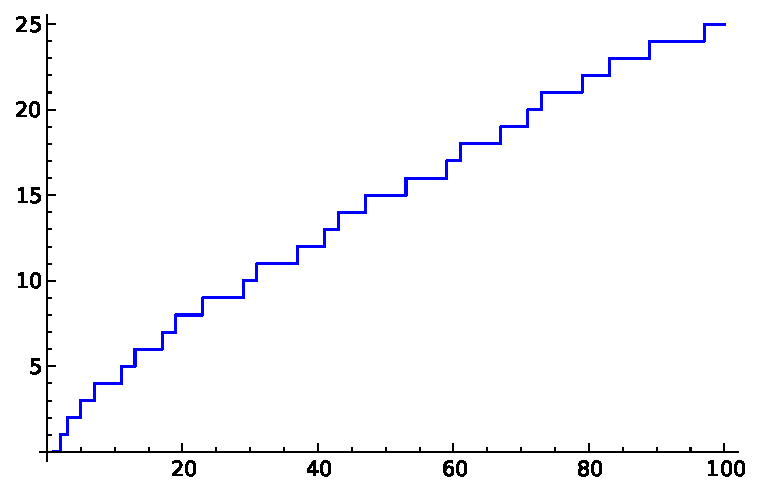
\includegraphics[width=.5\textwidth]{graphics/primepi100}
\end{center}

Based on heuristic evidence and numerical data, people conjectured (in
the 1700s) that the bumpy staircase $\pi(x)$ behaves somewhat like the
nice smooth function $x/\log(x)$.  The Prime Number Theorem makes this
precise; it is one of the deepest and most important theorems we have
about $\pi(x)$, and its proof is quite difficult.
\begin{theorem}[Prime Number Theorem]
We have $\pi(x) \sim x/\log(x)$, which means that
$$
 \lim_{x\to\infty} \frac{ x/\log(x) }{\pi(x)} = 1.
$$
\end{theorem}
This theorem means that if you want to use $x/\log(x)$ to estimate say
10 digits of $\pi(x)$, then there is definitely some $B$ such that for
all $x\geq B$, we have that $\pi(x)$ and $x/\log(x)$ have at least the
same first 10 digits.  However, the theorem itself makes no explicit
claim about what $B$ is; maybe it is $10^{30}$, or maybe it is
$10^{1000}$.

There is conjecturally a vastly better smooth function that estimates $\pi(x)$,
which is the special function $\Li(x)$:
$$
 \Li(x) = \int_{2}^x \frac{\d t}{\log(t)}.
$$
The following conjecture is widely believed, but so far nobody has a clue how
to prove it.  
\begin{conjecture}[Riemann Hypothesis]\label{conj:rh}
For all $x>2.01$, we have
$$
 |\pi(x) - \Li(x)| \leq \sqrt{x}\cdot \log(x).
$$
\end{conjecture}
In other words, if we estimate $\pi(x)$ using $\Li(x)$, then about
half of the digits will be right.  Moreover, there is no limit here;
this is a statement about all $x>2.01$, which is really amazing.

Some consider this conjecture to be the most important unsolved
problem in mathematics.  For example, it was selected as one of the
Clay Mathematics Institute million dollar prize problems:
\url{http://www.claymath.org/millennium/Riemann_Hypothesis/}

We illustrate the above conjecture using Sage. 
\begin{lstlisting}
sage: def rh(x):
...       pp = prime_pi(x)
...       print 'pi(x)         = %10.1f'%pp
...       print 'Li(x)         = %10.1f'%Li(x)
...       print 'x/log(x)      = %10.1f'%(x/math.log(x))
...       print 'sqrt(x)*log(x)= %10.1f'%(math.sqrt(x)*math.log(x))
...       print '|pi(x)-Li(x)| = %10.1f'%abs(pp - Li(x))
...       print '|pi(x)-x/l(x)|= %10.1f'%abs(pp - x/math.log(x))
...       
sage: rh(10^9)    
pi(x)         = 50847534.0
Li(x)         = 50849233.9
x/log(x)      = 48254942.4
sqrt(x)*log(x)=   655327.2
|pi(x)-Li(x)| =     1699.9
|pi(x)-x/l(x)|=  2592591.6
\end{lstlisting}

The following plot illustrates Conjecture~\ref{conj:rh}.  In the plot
$\pi(x)$ and $\Li(x)$ are visibly {\em on top of each other}!
\begin{lstlisting}
sage: x = var('x')
sage: B = 10^5
sage: G = (plot(prime_pi, 2, B) + plot(Li, 2, B, color='red') 
...             + plot(x/log(x), 2, B, color='green'))
sage: G += plot(lambda x: prime_pi(x) - math.sqrt(x)*math.log(x), 
...             2, B, color='black')
sage: G += plot(lambda x: prime_pi(x) + math.sqrt(x)*math.log(x), 
...             2, B, color='black')
sage: G
\end{lstlisting}
\begin{center}
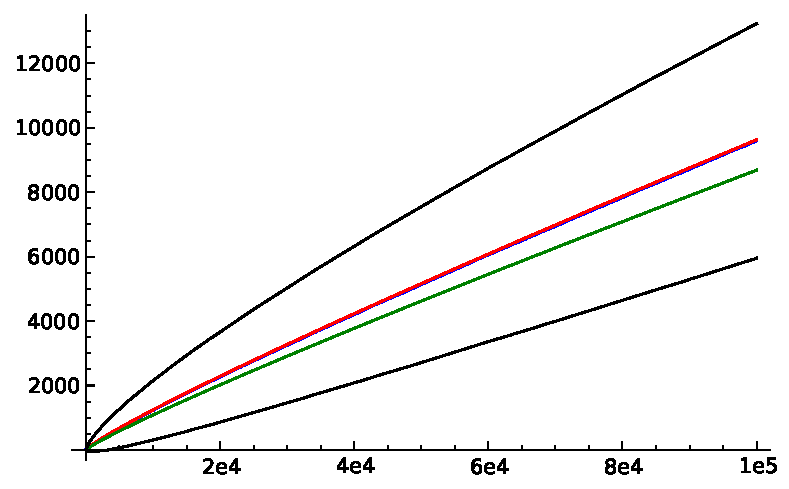
\includegraphics[width=.8\textwidth]{graphics/rhpic}
\end{center}



Conjecture~\ref{conj:rh} is typically stated in terms of a complex
analytic function called the {\em Riemann Zeta function}.
$$
  \zeta(s) = \sum_{n=1}^{\infty} \frac{1}{n^s} = \prod_{\text{primes $p$}} \frac{1}{1-p^{-s}}.
$$
The function $\zeta(s)$ has a (uniquely determined) analytic continuation to
$\C\setminus \{1\}$, and a simple pole at $s=1$.  In Sage, you can evaluate it anywhere
using the command \verb|zeta|:
\begin{lstlisting}
sage: zeta(2)
1/6*pi^2
sage: zeta(3+I)
zeta(I + 3)
\end{lstlisting}
Use the \verb|N| command or coercion to \verb|CC| (the complex field) to give a numerical answer.
\begin{lstlisting}
sage: CC(zeta(3+I))
1.10721440843141 - 0.148290867178175*I
sage: zeta(CC(3+I))
1.10721440843141 - 0.148290867178175*I
sage: N(zeta(3+I))
1.10721440843141 - 0.148290867178175*I
sage: N(zeta(3+I), 100)
1.1072144084314091956251002058 - 0.14829086717817534849076412567*I
\end{lstlisting} 

An equivalent version of Conjecture~\ref{conj:rh} is the following statement
about where the function $\zeta(s)$ takes the value $0$.
\begin{conjecture}\label{conj:rh2}
The zeros of $\zeta(s)$ with $\Re(s)\geq 0$ all satisfy $\Re(s)=1/2$.
\end{conjecture}

We can draw several plots of $\zeta(s)$, some of which illustrate the zeros of $\zeta(s)$.
\begin{lstlisting}
sage: complex_plot(zeta, (-30,30), (-30,30))
\end{lstlisting}
\begin{center}
% complex_plot(zeta, (-30,30), (-30,30)).save('zeta0.pdf')
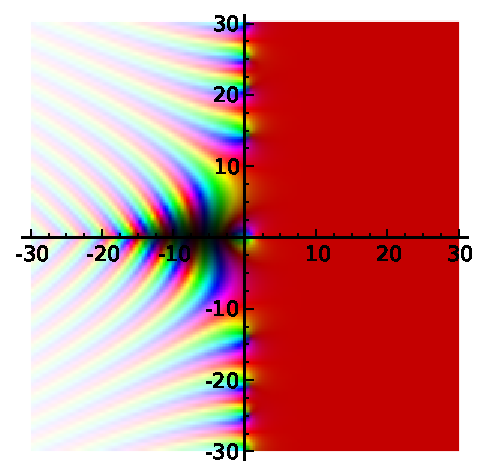
\includegraphics[width=.5\textwidth]{graphics/zeta0}
\end{center}


\begin{lstlisting}
sage: plot(lambda y: abs(zeta(1/2+I*y)), (0,50))
\end{lstlisting}
\begin{center}
% plot(lambda y: abs(zeta(1/2+I*y)), (0,50)).save('zeta1.pdf')
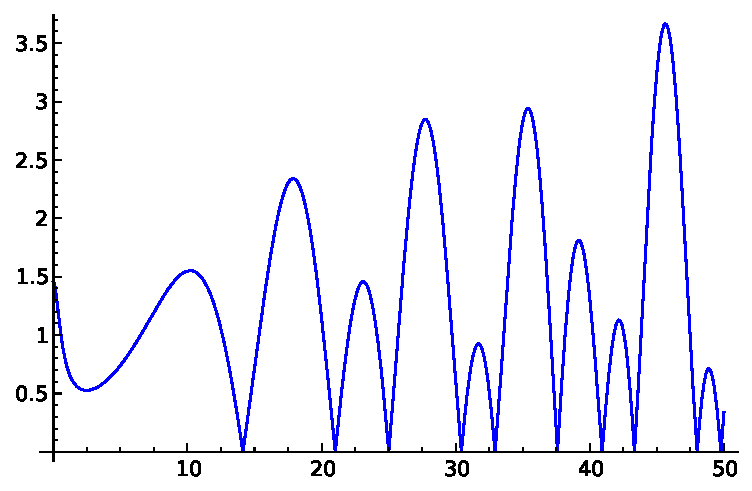
\includegraphics[width=.5\textwidth]{graphics/zeta1}
\end{center}

\begin{lstlisting}
sage: plot3d(lambda x, y: abs(zeta(x+I*y)), (.2,.7), (0,50), 
...             plot_points=100)
\end{lstlisting}
\begin{center}
% G = plot3d(lambda x, y: abs(zeta(x+I*y)), (.2,.7), (0,50), plot_points=100)
% G.save('zeta2.png', viewer='tachyon', aspect_ratio=[8,.3,1], zoom=1.4)
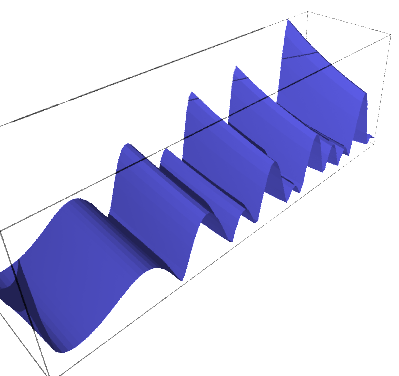
\includegraphics[width=.5\textwidth]{graphics/zeta2}
\end{center}


\section{Public-Key Cryptography: Diffie-Hellman}

(for this section, there is a lot more in my handwritten notes...)

\begin{verbatim}
<p>Naive modular exponentiation is not good.</p>
sage: 7^11
1977326743
sage: (7^11) % 13
2
<p>But Sage implements a vastly better algorithm.&nbsp;</p>
sage: a = Mod(18, 11); a
7
sage: type(a)
<type 'sage.rings.finite_rings.integer_mod.IntegerMod_int'>
sage: parent(a)
Ring of integers modulo 11
sage: 18 % 11
7
sage: parent(18 % 11)
Integer Ring
sage: type(18 % 11)
<type 'sage.rings.integer.Integer'>
sage: a^139299208340283408230482348032984023948
9
<p>Here is a bigger example.</p>
sage: p = next_prime(10^100); p
10000000000000000000000000000000000000000000000000000000000000000000000000000000000000000000000000267
sage: g = Mod(2, p)
sage: a = ZZ.random_element(p); a
3899462984078586138445766211121799052200774540320148812825084038333387229965957683578348930338929160
sage: g^a
7947388754511516576098430442932357966776257289140614732345836374084514192683933294095474801360397543
sage: timeit('g^a')
625 loops, best of 3: 71.1 µs per loop
<p>We illustrate the Diffie-Hellman key exchange.</p>
sage: @interact
sage: def _(bits=(5..1024), g=2, seed=(0..100)):
...       t = cputime()
...       set_random_seed(seed)
...       p = next_prime(2^(bits-1))
...       print "<html>"
...       print "p = %s"%p
...       a = ZZ.random_element(p)
...       b = ZZ.random_element(p)
...       print "a = %s"%a
...       print "b = %s"%b
...       g = Mod(g, p)
...       print "g^a (mod p) = %s"%(g^a)
...       print "g^b (mod p) = %s"%(g^b)
...       print "secret = %s = %s"%((g^a)^b, (g^b)^a)
...       print "total time = %s seconds"%cputime(t)
...       print "</html>"
sage: time next_probable_prime  (2^(1024-1))
89884656743115795386465259539451236680898848947115328636715040578866337902750481566354238661203768010560056939935696678829394884407208311246423715319737062188883946712432742638151109800623047059726541476042502884419075341171231440736956555270413618581675255342293149119973622969239858152417678164812112069763
Time: CPU 0.21 s, Wall: 0.21 s
<p>References:</p>
<ol>
<li>For math -- see <a href="http://wstein.org/ent " target="_blank">http://wstein.org/ent&nbsp;</a>(chapter 3).</li>
<li>More on cryptography using Sage -- see the book by David Kohel that is <a href="http://sagemath.org/library-publications.html#books" target="_blank">listed here</a>.</li>
<li>There is a library called <a href="http://www.dlitz.net/software/pycrypto/" target="_blank">PyCrypto</a> that is included with Sage.&nbsp;</li>
</ol>
\end{verbatim}


\section{Elliptic Curves and the Birch and Swinnerton-Dyer Conjecture}\label{sec:bsd}

\subsection{Fields}
A {\em field} is a set of objects equipped with rules for multiplication and
addition that satisfy certain axioms (for example, every nonzero
element has an inverse).   
Standard examples of fields include  the field $\C$ of all complex numbers and the
field $\Q$ of all rational numbers.  Also, for every prime number
$p$ we have the {\em finite field}
$$
 \F_p = \{0, 1, 2, \ldots, p-2, p-1\}
$$
of numbers modulo $p$.  In the field $\F_p$, arithmetic is defined by
multiply or adding two numbers, then taking the remainder modulo $p$.

\subsection{Elliptic Curves}
\begin{definition}[Elliptic Curve]
  An {\em elliptic curve} over a field $K$ is a curve defined by an
  equation $y^2 = x^3 + ax + b$ with $a,b\in K$ such that the cubic
  $x^3 +ax+b$ has distinct roots; equivalently, the discriminant $-4
  a^{3} - 27 b^{2}$ of the cubic is nonzero.
\end{definition}

Suppose now that $E$ is an elliptic curve over a field $K$.  Then the set of $K$-rational
points on $E$ is
$$
  E(K) = \{(X,Y) \in K \times K : Y^2 = X^3 + aX + b \} \cup \{\cO\}.
$$
The extra point $\cO$ should be thought of as being ``at infinity'' and is included
since we view $E$ as a curve in the ``projective plane''. 

There is a natural way to define a way off {\em adding together} two
elements $P,Q \in E(K)$ to get another element $R =P+Q\in E(K)$, thus
generating possibly new points. This is the ``chord and tangent'' procedure;
the following diagram illustrates using it to compute $R=P+Q=(0,1)+(-1,0)=(2,-3)$.

\begin{lstlisting}
sage: E = EllipticCurve([0,1])
sage: P = E([0,1]); Q = E([-1,0]); R = P+Q; mR = -R
sage: G = E.plot(-1.5,2.5, plot_points=300)
sage: v = [(0,1), (-1,0), (2,-3), (2,3)]
sage: G += points(v, pointsize=50, color='black')
sage: G += line([(-1.5,-.5), (2.5,3.5)], color='red')
sage: G += text("P", (-1.2,.3), color='black')
sage: G += text("Q", (-.3,1.3), color='black')
sage: G += text("-R", (1.8,3.2), color='black')
sage: G += text("R=P+Q", (1.3,-2.85), color='black')
sage: G += line([(2,3.5), (2,-3.5)], color='green')
sage: G.show(gridlines=True, aspect_ratio=1)
\end{lstlisting}
\begin{center}
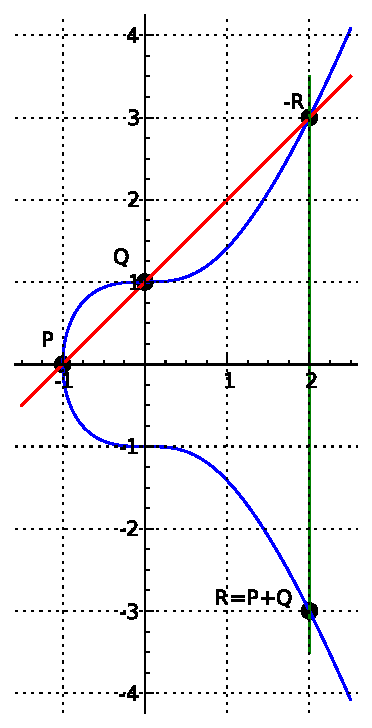
\includegraphics[width=.4\textwidth]{graphics/group_law}
\end{center}

When $K=\Q$ is the rational numbers, there is an amazing theorem about
$E(K)$.
\begin{theorem}[Mordell]
Let $E$ be any elliptic curve over $\Q$.
Then there are finitely many points $P_1,\ldots, P_k$ in $E(\Q)$ such
that {\em every} point in $E(\Q)$ is of the form
$n_1 P_1 + \cdots + n_k P_k$ for
some integers $n_1, \ldots, n_k \in \Z$.
\end{theorem}

Mordell's theorem means that $E(\Q)$ is a finitely generated abelian
group, so $E(\Q)$ is isomorphic to $\Z^r \oplus T$, for some finite
group $T$, and some nonnegative integer $r$.  The number $r =
\rank(E)$ is called the {\em rank} of $E$ and is a fundamental and
mysterious invariant of $E$. 

\begin{openproblem}\label{prob:rank}
  Give an algorithm that takes as input an elliptic curve $E$ over
  $\Q$ and outputs the rank of $E$.
\end{openproblem}

Problem~\ref{prob:rank} goes back over 1000 years, making it perhaps
the oldest {\em ``interesting''} problem in all of mathematics, where
the problem is interesting because of its connections to many ideas in
modern number theory, and the numerous partial results that
mathematicians have obtained.  In particular, around 1000 years ago
the Arabs asked for an algorithm to decide whether or not an integer
$n$ is the area of a rational right triangle, i.e., a right triangle
all three of whose side lengths are rational numbers.  The connection with
Problem~\ref{prob:rank} arises because $n$ is the area of a rational
right triangle if and only if the rank of the elliptic curve $y^2 =
x^3 + n^2 x$ is positive.


\subsection{Birch and Swinnerton-Dyer}
In the 1960s two British mathematicians, Bryan Birch and Sir Peter
Swinnerton-Dyer (BSD), had an amazing idea related to
Problem~\ref{prob:rank}.  After a huge amount of work and
difficult hard won 1960s computer use, they obtained precise
data relating two quantities for many elliptic curves.
Let $N_p = \# E(\F_p)$, where $\# E(\F_p)$ is the number
of points on the elliptic curve obtained by reducing the equation that
defines $E$ modulo $p$, when this makes sense. 
$$
  \rank(E) \longleftrightarrow f_E(M),
$$
where
$$
f_E(M) = \prod_{\text{good primes }p< M} \frac{N_p}{p}.
$$
This function is something that is dramatically simpler to contemplate
computing than $\rank(E)$.  You simply reduce the equation that
defines $E$ modulo $p$, and count all the solutions modulo $p$ to the
reduced equation.  It is easy to come up with a (slow) algorithm to
do that for any given $p$.

\begin{center}
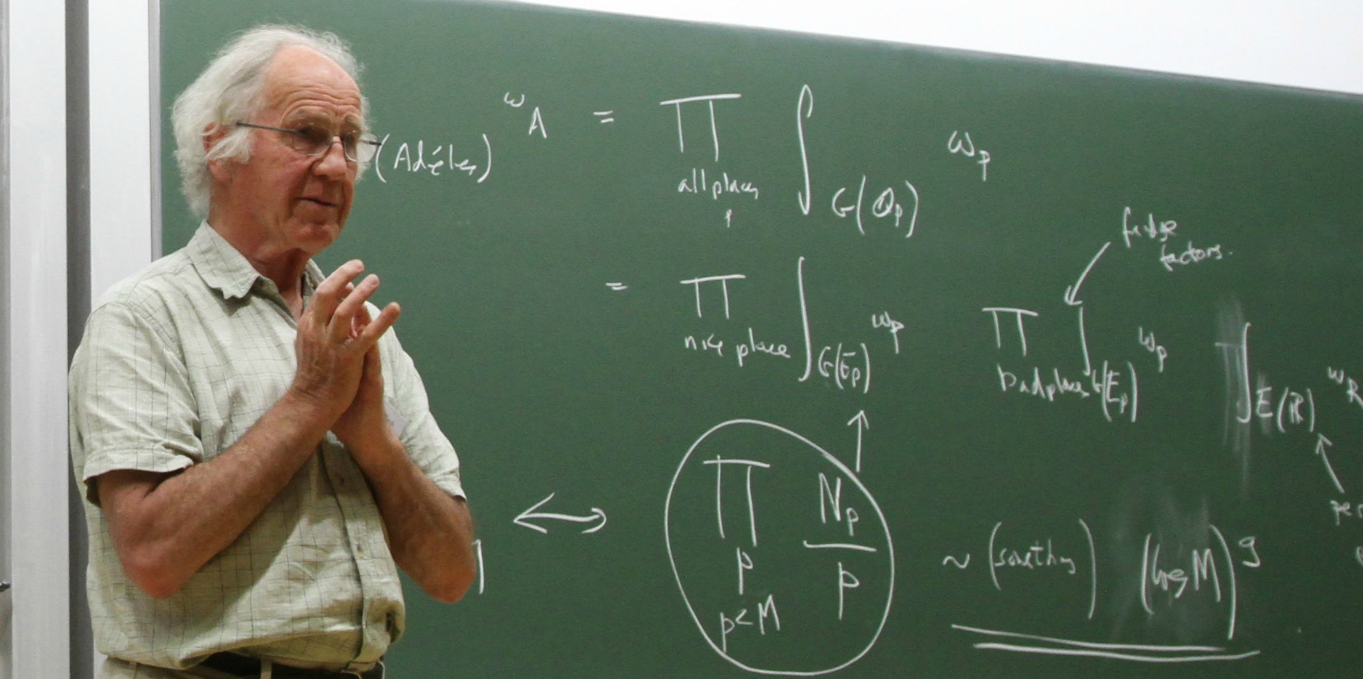
\includegraphics[width=.9\textwidth]{graphics/birch}\\
Birch explaining the conjecture in Cambrige on May 4, 2011
\end{center}

We will compute $f_E(M)$ in Sage using the following:
\begin{lstlisting}
def f(E,M):
    N = E.conductor()
    return prod(E.Np(p)/float(p) for p in primes(M) if N%p)
\end{lstlisting}
  
BSD considered mainly curves of the form $y^2 = x^3 + b$, with $b$ an integer.
For example, we have the following table for various values of $b$:
\begin{lstlisting}
for b in [1,2,-11,-6,316]:
    E = EllipticCurve([0,b])
    v = (b, E.rank(), f(E,10^3), f(E,10^4), f(E,10^6))
    print '%4s%4s%10.3f%10.3f%10.3f'%v


   1   0     1.895     2.060     1.849
   2   1     6.804     8.735    11.693
 -11   2    36.523    49.215   143.102
  -6   0     0.461     0.551     1.013
 316   3   100.158   261.144   879.231
\end{lstlisting}

  

Here is a photo I snapped of the very piece of paper on which BSD
came up with the basic idea of matching the ranks up with the behavior
of $f_E(M)$ (do not ask me to explain it):
\begin{center}
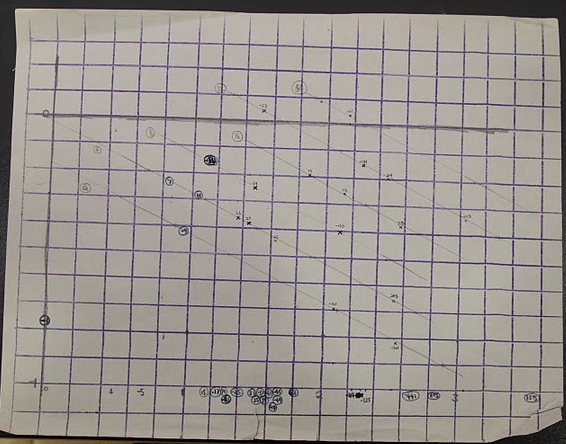
\includegraphics[width=.8\textwidth]{graphics/birch_paper}
\end{center}

What they found was that by eyeballing the plots of $f_E(M)$, they were able
in practice to predict the rank.   Incidentally, we can plot $f_E(M)$ in
Sage using the following code:
\begin{lstlisting}
def f_plot(E, M, **kwds):
    N = E.conductor()
    v = [(0,1)]
    pr = 1
    for p in primes(M):
        if N%p:
            pr *= E.Np(p)/float(p)
            v.append((p, v[-1][1]))
            v.append((p, pr))
    return line(v, **kwds)

B = 10^5
show(f_plot(EllipticCurve([0,1]), B, color='red') + 
    f_plot(EllipticCurve([0,2]), B, color='blue') + 
    f_plot(EllipticCurve([0,-11]), B, color='green') + 
    f_plot(EllipticCurve([0,-6]), B, color='orange') + 
    f_plot(EllipticCurve([0,316]), B, color='purple')
)    
\end{lstlisting}
\begin{center}
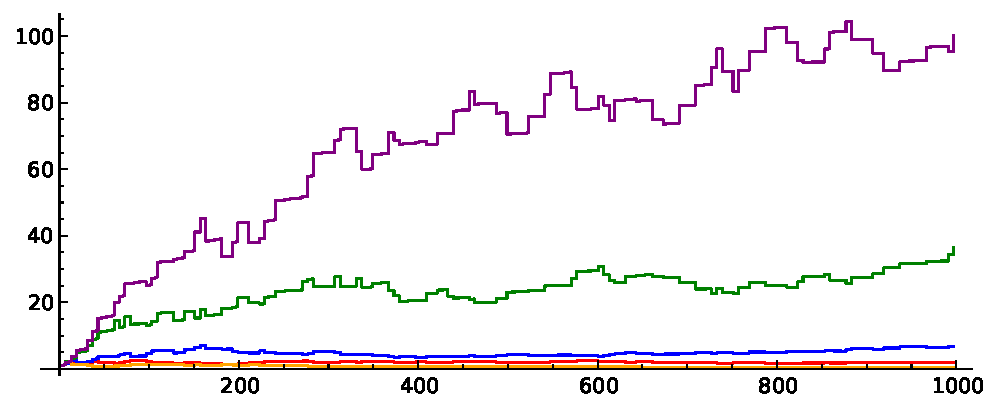
\includegraphics[width=.8\textwidth]{graphics/bsd_plot}
\end{center}

I hope you will agree that looking at the above pictures suggests the
rank... but certainly doesn't feel rock solid and precise.
Fortunately, there is another approach to the same problem that
involves an object much like the Riemann Zeta function, which appeared
above in Section~\ref{sec:bsd}.

Fix an elliptic curve $E$.  For each prime number $p$, set $a_p = p+1 - N_p$.  
Let
\begin{equation}\label{eqn:L}
  L^*(E,s) = \prod_{p} \frac{1}{1 - a_p p^{-s} + p^{1-2s}}.
\end{equation}
\begin{remark}
There is also a way to define factors for all primes $p$, and one obtains a function
that we denote $L(E,s)$.   For the conjecture we make below, it makes no difference
whether we use $L^*(E,s)$ or $L(E,s)$.
\end{remark}

A big theorem proved in 2000, but proved in many special cases already in 1960s is:
\begin{theorem}
The function $L(E,s)$ has a unique analytic continuation to the whole complex plane. 
\end{theorem}
In other words, despite the right hand side of \eqref{eqn:L} possibly
not converging, there is a natural and meaningful ``nice'' way of
making sense of $L(E,s)$ for any complex number $s$.
The reason $L(E,s)$ is so relevant to the function $f_E(M)$ that we considered
above is that {\em formally}\footnote{And in fact this equality is probably true only true up to a factor of $\sqrt{2}$...}
$$
 L(E,1) ``=\text{''} \prod_p \frac{1}{1- a_p p^{-1}  + p^{1-2}} = \prod_p  \frac{p}{p - a_p + 1} = 
   \prod_{p} \frac{p}{N_p} ``= \frac{1}{f_E(\infty)}\text{''}.
$$

Motivated by the above formal observation and their other data, BSD
made the following conjecture:
\begin{conjecture}[Birch and Swinnerton-Dyer]\label{conj:bsd}
Let $E$ be an elliptic curve over $\Q$.  Then
$$
  \ord_{s=1} L(E,s) = \rank(E).
$$
\end{conjecture}
This is a Clay Million Dollar prize problem:
\url{http://www.claymath.org/millennium/Birch_and_Swinnerton-Dyer_Conjecture/}.

The work of many, many people over several decades has resulted in the
following theorem:
\begin{theorem}
If $\ord_{s=1} L(E,s) \leq 1$, then Conjecture~\ref{conj:bsd} holds for $E$.
\end{theorem}

Sage is good at computing with $L(E,s)$.  For example,
\begin{lstlisting}
sage: E = EllipticCurve([0,-6])
sage: L = E.lseries().dokchitser()
sage: L(2)
0.970573503589685
sage: L(1)
1.80166139420421
sage: L(1+I)
1.37330247586099 + 0.672104565160637*I
sage: L.taylor_series(1, 5)
1.80166139420421 - 4.34358857895219*z + 10.6996108328594*z^2 
   - 16.6581015345210*z^3 + 17.7188237405279*z^4 + O(z^5)
\end{lstlisting}
Here is an example of rank $2$:
\begin{lstlisting}
sage: E = EllipticCurve([0,-11])
sage: L = E.lseries().dokchitser()
sage: L.taylor_series(1, 5)
2.66270802215019e-23 + (-6.18778237886993e-23)*z 
     + 5.92327478382316*z^2 - 13.7649096437350*z^3 
     + 17.0105571907034*z^4 + O(z^5)
\end{lstlisting}
Finally, here is an example of rank $3$:
\begin{lstlisting} 
sage: E = EllipticCurve([0,316])
sage: E.rank()
sage: L = E.lseries().dokchitser()
sage: L.taylor_series(1, 5)
(8.21208956591497e-23)*z + (-3.64556152695356e-22)*z^2 
   + 25.3581351256025*z^3 - 112.571399845523*z^4 + O(z^5)
sage: E.analytic_rank() # order of vanishing of L
3
\end{lstlisting}


Though we can numerically evaluate $L(E,s)$ at any point to any number
of digits, we do not have a way in general to provably compute
$\ord_{s=1} L(E,s)$.  For example, we may suspect that $\ord_{s=1}
L(E,s)=4$ since {\em numerically} to 10,000 digits (say) we find that
$L^{(k)}(E,1)=0.00000...$ for $k=0,1,2,3$, but this is not a proof.
\begin{openproblem}
  Verify with proof Conjecture~\ref{conj:bsd} for one single elliptic
  curve of rank $4$, e.g., for the curve $y^2 = x^3 - 102627x +
  12560670$.
\end{openproblem}






%%%%%%%%%%%%%%%%%%%%%%%%%%%%%%%%%%%%%%%%%%%%%%%%%%%%%%%%%%%%%%%%
\chapter{Statistics}

\section{Using R with Sage}\label{ch:R}
TODO:
\begin{verbatim}
<p>See <a href="http://rpy.sourceforge.net/rpy2/doc-2.0/html/introduction.html" target="_blank">http://rpy.sourceforge.net/rpy2/doc-2.0/html/introduction.html</a>. &nbsp;</p>
sage: %auto
sage: import rpy2.robjects as robjects
sage: R = robjects.r
<p>We get pi from the R namespace.</p>
sage: v = R['pi']; v
<RVector - Python:0x433e320 / R:0x4fd90c8>
<p>Note that we have to explicitly use print to see a nice representation:</p>
sage: print v
[1] 3.141593
<p>There is a pexpect interface to r called "r" by default when you start Sage. &nbsp;This tutorial is not about that interface, but instead about the C library interface called rpy2, which is much faster and more robust.</p>
sage: r
R Interpreter
sage: r('2 + 3')   # the pexpect interface
[1] 5
sage: import rpy2.robjects as robjects
sage: R = robjects.r
sage: print R('2 + 3')  # the rpy2 cython interface (note the import!)
[1] 5
sage: R("""
sage: a = 5
sage: b = 7
sage: c = a + b""")
sage: print R("c")
[1] 12
sage: timeit("r('2+3')")
625 loops, best of 3: 1.44 ms per loop
sage: timeit("R('2+3')")
625 loops, best of 3: 650 µs per loop
sage: timeit("pari('2+3')")
625 loops, best of 3: 5.72 µs per loop
<p>(frankly, I'm shocked at how slow the rpy2 interface actually is...!)</p>
<p>This is how to get started with rpy2:</p>

<p>Beware the preparser:</p>
sage: v = R['pi']; v
<RVector - Python:0x433ec20 / R:0x4fd90c8>
sage: print v
[1] 3.141593
sage: repr(v)
'<RVector - Python:0x433dcf8 / R:0x48e3178>'
sage: str(v)
'[1] 3.141593'
sage: w =  v + int(1); print w
[1] 3.141593 1.000000
sage: w[0]
3.1415926535897931
sage: v + 3
Traceback (most recent call last):
...
ValueError: Nothing can be done for the type <type 'sage.rings.integer.Integer'> at the moment.
<p>And note again that v is a vector not a number.</p>
sage: print v + int(3)
[1] 3.141593 3.000000
sage: print v[0] + int(3)
6.14159265359
<p>WARNING: &nbsp;Python indexing starts at 0 and R indexing starts at 1.</p>
sage: print R('c(5,2,-3)[1]')
[1] 5
sage: timeit('R("f <- function(r) { 2 * pi * r }")')
625 loops, best of 3: 460 µs per loop
<p>Define a function in R:</p>
sage: R("f <- function(r) { 2 * pi * r }")
<RFunction - Python:0x433f440 / R:0x529ec00>
<p>Now call the function:</p>
sage: print R("f(3)")
[1] 18.84956
<p>The function is now defined in the global R namespace:</p>
sage: r_f = R['f']
sage: print r_f(int(3))
[1] 18.84956
sage: timeit('r_f(int(3))')
625 loops, best of 3: 41.4 µs per loop
sage: print R("f")
function(r) { 2 * pi * r }
<p>Most R objects have a string representation that can be directly parsed by R, which can be handy.</p>
sage: letters = R['letters']
sage: print letters.r_repr()
c("a", "b", "c", "d", "e", "f", "g", "h", "i", "j", "k", "l", 
"m", "n", "o", "p", "q", "r", "s", "t", "u", "v", "w", "x", "y", 
"z")
<p>Here is an example of how we might use this:</p>
sage: rcode = 'paste(%s, collapse="-")' %(letters.r_repr())
sage: print R(rcode)
[1] "a-b-c-d-e-f-g-h-i-j-k-l-m-n-o-p-q-r-s-t-u-v-w-x-y-z"
sage: timeit('robjects.IntVector(range(10))')
625 loops, best of 3: 9.65 µs per loop
sage: time w = robjects.IntVector(range(10^6))
Time: CPU 0.74 s, Wall: 0.74 s
sage: time print R['mean'](w)
[1] 499999.5
Time: CPU 0.16 s, Wall: 0.17 s
sage: time print R['sd'](w)
[1] 288675.3
Time: CPU 0.18 s, Wall: 0.18 s
sage: time w = r(range(10^3))
Time: CPU 1.12 s, Wall: 2.56 s
sage: time z = pari(range(10^6))
Traceback (most recent call last):
...
KeyboardInterrupt: evaluating PARI string
__SAGE__
<h2>Vectors</h2>
<p>Vectors are an important basic data structure in R:</p>
sage: print robjects.StrVector(['abc', 'def'])
[1] "abc" "def"
sage: print robjects.IntVector([1, 2, 3])
[1] 1 2 3
sage: print robjects.FloatVector([1.1, 2.2, 3.3])
[1] 1.1 2.2 3.3
<p>You can also create R matrices, which are R vectors with a dim attribute:</p>
sage: v = robjects.FloatVector([1.1, 2.2, 3.3, 4.4, 5.5, 6.6])
sage: m = R['matrix'](v, nrow = int(2))
sage: print m
     [,1] [,2] [,3]
[1,]  1.1  3.3  5.5
[2,]  2.2  4.4  6.6
<h2>R functions</h2>
<p>The above illustrates how to call an R function. &nbsp;You get it from the R namespace, then call it in the standard way. &nbsp;Here's another example:</p>
sage: v = robjects.IntVector([1..10])
sage: print R['sum']
function (..., na.rm = FALSE)  .Primitive("sum")
sage: ans = R['sum'](v)
sage: ans
<RVector - Python:0x4368368 / R:0x4e63188>
sage: print ans
[1] 55
sage: ans[0]
55
sage: R['sum'](v)[0]    # [0] since result is a vector of length 1
55
sage: R['mean'](v)[0]
5.5
sage: R['sd'](v)[0]
3.0276503540974917
sage: sd = R['sd']
sage: timeit('sd(v)')
625 loops, best of 3: 280 µs per loop
sage: timeit("R['sd'](v)")
625 loops, best of 3: 237 µs per loop
<p>You can also pass in keywords:</p>
sage: rsort = R['sort']
sage: print rsort(v, decreasing=True)
 [1] 10  9  8  7  6  5  4  3  2  1
<p>GOTCHA: In R variable names with dots in them are allowed, but in Python they are not. &nbsp; The example below illustrates how to deal with this (use **kwds). &nbsp;In this example, we make an R vector with a "NA" in it, which means we don't know that entry; the na.rm option to R's sum command controls how it behaves on lists with NA's in them.</p>
sage: v = R('c(1,NA,2,3)')
sage: print v
[1]  1 NA  2  3
sage: print R['sum']
function (..., na.rm = FALSE)  .Primitive("sum")
sage: rsum = R['sum']
sage: print rsum(v)
[1] NA
<p>Directly in R, we would just type na.rm=TRUE. &nbsp;In Python this does not make sense.</p>
sage: print R('sum( c(1,NA,2,3), na.rm=TRUE )')
[1] 6
sage: print rsum(v, na.rm=True)   # boom!
Traceback (most recent call last):
...
SyntaxError: keyword can't be an expression
sage: f(*[5,,7])
33
<p>So we use **kwds, which works fine:</p>
sage: a = {'na.rm':True}
sage: print R['sum'](v, **a)
[1] 6
sage: def f(a, b, c):
...       return a + 2*b + 3*c
...
sage: args = (5,)
sage: kwds = {'b':7, 'c':13}
sage: f(*args, **kwds)
58
sage: def g(*scott, **alex):
...       print scott, alex
...       return f(*scott, **alex)
sage: g(1,2,c=3)
(1, 2) {'c': 3}
14
sage: f( *(3, 8), **{'c':2})
25
sage: f( 2, *(5,), **{'c':1})
15
<h2>Plotting using Rpy2:</h2>
<ol>
<li>Call the R.png function to tell R where the output image should be saved (and what size it should be).</li>
<li>Draw plots on the canvas until done.</li>
<li>Tell R to turn the plotting device off, which causes the output file to be written. &nbsp;</li>
</ol>
<p>IMPORTANT: This must all happen in the same notebook cell. &nbsp;Otherwise the output file gets written in temp directory for a cell that was already evaluated, and the plot may not appear.</p>
sage: x = robjects.IntVector(range(50))
sage: y = R.rnorm(len(x))     # normal random numbers
sage: # 300r = "raw Python int" (no preparser)
sage: R.png('sage.png', width=600r, height=300r)   
sage: R.plot(x, y, xlab="x", ylab="rnorm", col="red")
sage: _ = R['dev.off']()   # "_ =" to suppress printing
<p>Interact works, of course.</p>
sage: @interact 
sage: def _(points=(10..1000)):
...       x = robjects.IntVector(range(points)); y = R.rnorm(int(points))
...       R.png('sage.png', width=600r, height=300r)
...       R.plot(x, y, xlab="x", ylab="rnorm", col="blue")
...       R['dev.off']()
<p><strong>Warning again -- Do NOT do this:</strong> call dev.off in a separate cell!</p>
sage: # intentionally broken!
sage: x = robjects.IntVector(range(50))
sage: y = R.rnorm(len(x))     # normal random numbers
sage: R.png('sage.png', width=600r, height=300r)
sage: R.plot(x, y, xlab="runif", ylab="foo/bar", col="red")
<RObject - Python:0x434b488 / R:0x42a6758>
sage: R['dev.off']()
<RVector - Python:0x434b128 / R:0x551b408>
<h2>A More Nontrivial Example</h2>
<p>&nbsp;</p>

<p>This is how we would do this directly in R, which we can use from Sage by using the "%r" mode in the notebook (or r.eval("""...""")):</p>
sage: %r
sage: ctl <- c(4.17,5.58,5.18,6.11,4.50,4.61,5.17,4.53,5.33,5.14)
sage: trt <- c(4.81,4.17,4.41,3.59,5.87,3.83,6.03,4.89,4.32,4.69)
sage: group <- gl(2, 10, 20, labels = c("Ctl","Trt"))
sage: weight <- c(ctl, trt)
sage: anova(lm.D9 <- lm(weight ~ group))
sage: summary(lm.D90 <- lm(weight ~ group - 1))# omitting intercept
Analysis of Variance Table

Response: weight
          Df Sum Sq Mean Sq F value Pr(>F)
group      1 0.6882 0.68820  1.4191  0.249
Residuals 18 8.7293 0.48496               

Call:
lm(formula = weight ~ group - 1)

Residuals:
    Min      1Q  Median      3Q     Max 
-1.0710 -0.4938  0.0685  0.2462  1.3690 

Coefficients:
         Estimate Std. Error t value Pr(>|t|)    
groupCtl   5.0320     0.2202   22.85 9.55e-15 ***
groupTrt   4.6610     0.2202   21.16 3.62e-14 ***
---
Signif. codes:  0 ‘***’ 0.001 ‘**’ 0.01 ‘*’ 0.05 ‘.’ 0.1 ‘ ’ 1 

Residual standard error: 0.6964 on 18 degrees of freedom
Multiple R-squared: 0.9818,	Adjusted R-squared: 0.9798 
F-statistic: 485.1 on 2 and 18 DF,  p-value: < 2.2e-16 
<p>Next, we do the same computation, but via rpy2 (which is unfortunately more complicated):</p>
sage: ctl = robjects.FloatVector([4.17,5.58,5.18,6.11,4.50,4.61,5.17,4.53,5.33,5.14])
sage: trt = robjects.FloatVector([4.81,4.17,4.41,3.59,5.87,3.83,6.03,4.89,4.32,4.69])
sage: group = R.gl(2r, 10r, 20r, labels = ["Ctl","Trt"])
sage: weight = ctl + trt
sage: robjects.globalEnv["weight"] = weight
sage: robjects.globalEnv["group"] = group
sage: lm_D9 = R.lm("weight ~ group")
sage: print(R.anova(lm_D9))
Analysis of Variance Table

Response: weight
          Df Sum Sq Mean Sq F value Pr(>F)
group      1 0.6882 0.68820  1.4191  0.249
Residuals 18 8.7293 0.48496               
sage: lm_D90 = R.lm("weight ~ group - 1")
sage: v = R.summary(lm_D90)
sage: print(v)
Call:
function (formula, data, subset, weights, na.action, method = "qr", 
    model = TRUE, x = FALSE, y = FALSE, qr = TRUE, singular.ok = TRUE, 
    contrasts = NULL, offset, ...) 
{
    ret.x <- x
    ret.y <- y
    cl <- match.call()
    mf <- match.call(expand.dots = FALSE)
    m <- match(c("formula", "data", "subset", "weights", "na.action", 
        "offset"), names(mf), 0L)
    mf <- mf[c(1L, m)]
    mf$drop.unused.levels <- TRUE
    mf[[1L]] <- as.name("model.frame")
    mf <- eval(mf, parent.frame())
    if (method == "model.frame") 
        return(mf)
    else if (method != "qr") 
        warning(gettextf("method = '%s' is not supported. Using 'qr'", 
            method), domain = NA)
    mt <- attr(mf, "terms")
    y <- model.response(mf, "numeric")
    w <- as.vector(model.weights(mf))
    if (!is.null(w) && !is.numeric(w)) 
        stop("'weights' must be a numeric vector")
    offset <- as.vector(model.offset(mf))
    if (!is.null(offset)) {
        if (length(offset) != NROW(y)) 
            stop(gettextf("number of offsets is %d, should equal %d (number of observations)", 
                length(offset), NROW(y)), domain = NA)
    }
    if (is.empty.model(mt)) {
        x <- NULL
        z <- list(coefficients = if (is.matrix(y)) matrix(, 0, 
            3) else numeric(0L), residuals = y, fitted.values = 0 * 
            y, weights = w, rank = 0L, df.residual = if (is.matrix(y)) nrow(y) else length(y))
        if (!is.null(offset)) {
            z$fitted.values <- offset
            z$residuals <- y - offset
        }
    }
    else {
        x <- model.matrix(mt, mf, contrasts)
        z <- if (is.null(w)) 
            lm.fit(x, y, offset = offset, singular.ok = singular.ok, 
                ...)
        else lm.wfit(x, y, w, offset = offset, singular.ok = singular.ok, 
            ...)
    }
    class(z) <- c(if (is.matrix(y)) "mlm", "lm")
    z$na.action <- attr(mf, "na.action")
    z$offset <- offset
    z$contrasts <- attr(x, "contrasts")
    z$xlevels <- .getXlevels(mt, mf)
    z$call <- cl
    z$terms <- mt
    if (model) 
        z$model <- mf
    if (ret.x) 
        z$x <- x
    if (ret.y) 
        z$y <- y
    if (!qr) 
        z$qr <- NULL
    z
}(formula = "weight ~ group - 1")

Residuals:
    Min      1Q  Median      3Q     Max 
-1.0710 -0.4938  0.0685  0.2462  1.3690 

Coefficients:
         Estimate Std. Error t value Pr(>|t|)    
groupCtl   5.0320     0.2202   22.85 9.55e-15 ***
groupTrt   4.6610     0.2202   21.16 3.62e-14 ***
---
Signif. codes:  0 ‘***’ 0.001 ‘**’ 0.01 ‘*’ 0.05 ‘.’ 0.1 ‘ ’ 1 

Residual standard error: 0.6964 on 18 degrees of freedom
Multiple R-squared: 0.9818,	Adjusted R-squared: 0.9798 
F-statistic: 485.1 on 2 and 18 DF,  p-value: < 2.2e-16 
sage: print(lm_D9.names)
 [1] "coefficients"  "residuals"     "effects"       "rank"         
 [5] "fitted.values" "assign"        "qr"            "df.residual"  
 [9] "contrasts"     "xlevels"       "call"          "terms"        
[13] "model"        
sage: print(lm_D9.r['coefficients'])
$coefficients
(Intercept)    groupTrt 
      5.032      -0.371 
<p>You could also use rpy2 as follows to do this computation:</p>
sage: R("""
sage: ctl <- c(4.17,5.58,5.18,6.11,4.50,4.61,5.17,4.53,5.33,5.14)
sage: trt <- c(4.81,4.17,4.41,3.59,5.87,3.83,6.03,4.89,4.32,4.69)
sage: group <- gl(2, 10, 20, labels = c("Ctl","Trt"))
sage: weight <- c(ctl, trt)
sage: print(anova(lm.D9 <- lm(weight ~ group)))
sage: print(summary(lm.D90 <- lm(weight ~ group - 1)))
sage: """)
Analysis of Variance Table

Response: weight
          Df Sum Sq Mean Sq F value Pr(>F)
group      1 0.6882 0.68820  1.4191  0.249
Residuals 18 8.7293 0.48496               

Call:
lm(formula = weight ~ group - 1)

Residuals:
    Min      1Q  Median      3Q     Max 
-1.0710 -0.4938  0.0685  0.2462  1.3690 

Coefficients:
         Estimate Std. Error t value Pr(>|t|)    
groupCtl   5.0320     0.2202   22.85 9.55e-15 ***
groupTrt   4.6610     0.2202   21.16 3.62e-14 ***
---
Signif. codes:  0 ‘***’ 0.001 ‘**’ 0.01 ‘*’ 0.05 ‘.’ 0.1 ‘ ’ 1 

Residual standard error: 0.6964 on 18 degrees of freedom
Multiple R-squared: 0.9818,	Adjusted R-squared: 0.9798 
F-statistic: 485.1 on 2 and 18 DF,  p-value: < 2.2e-16 
<h2>Data Frames</h2>
<p>In R a "data frame" is an array of values with labeled rows and columns (like part of a spreadsheet). &nbsp;Typically one thinks of a data frame as a table where the rows are observations and the columns are variables.</p>
<p>You can create a data frame using the data.frame R function:</p>
sage: d = {'value': robjects.IntVector((24,25,26)),
...        'letter': robjects.StrVector(('x', 'y', 'z'))}
...
sage: dataf = R['data.frame'](**d)
sage: print(dataf)
  letter value
1      x    24
2      y    25
3      z    26
sage: type(dataf)
<class 'rpy2.robjects.RDataFrame'>
<p>Get each column:</p>
sage: print dataf.r['letter']
  letter
1      x
2      y
3      z
sage: print dataf.r['value']
  value
1    24
2    25
3    26
<p>Labels for the rows:</p>
sage: print dataf.rownames()
[1] "1" "2" "3"
<p>Labels for the columns:</p>
sage: print dataf.colnames()
[1] "letter" "value" 
<h2>Converting Between Numpy and RPy2</h2>
<p>If you are using rpy2 and Sage together to deal with large real-world data sets, then it is critical that you can quickly move data back and forth. &nbsp; If you're working with big data in Sage, you're probably using numpy arrays. &nbsp;Fortunately, there is a way to very quickly convert a big numpy array to an R vector and conversely, as we illustrate below.</p>
<p>NOTE: The rpy2 documentation suggests doing "import rpy2.robjects.numpy2ri" but this is broken (at least with the versions of R, rpy2, and numpy in Sage), and gives totally wrong results. &nbsp;So just explicitly use FloatVector, etc., as illustrated below.</p>
sage: import numpy
sage: a = numpy.array([[1,2],[3,4]], dtype=float)
sage: v = numpy.arange(5)
sage: print R(v)
Traceback (most recent call last):
...
ValueError: Nothing can be done for the type <type 'numpy.ndarray'> at the moment.
sage: print(robjects.FloatVector(v))
[1] 0 1 2 3 4
sage: import rpy2.robjects.numpy2ri
sage: print R(numpy.array([[1,2],[3,4]], dtype=float))
[1] 4
<p>... CRAP, this seems to be just totally broken in rpy2. &nbsp;Maybe it is fixed in a newer version. &nbsp;Sorry folks.</p>
\end{verbatim}



\chapter{Abstract Algebra}

\section{Groups, Rings and Fields}
\begin{verbatim}
<p>The first page of "abstract mathematics" that I ever saw, accidentally misfiled in a the computer book section of Bookman's in Flagstaff.  (Burton W. Jones's "An Introduction to Modern Algebra", 1975.)</p>
<p><img src="data/burton.png" alt="" /></p>
<h2>Groups</h2>
<p>A group is a set $G$ equipped with a binary operation $G \times G \to G$ that we write as a dot below that has three properties:</p>
<ol>
<li><strong>Associativity</strong>: &nbsp;$(a\cdot b)\cdot c = a\cdot(b\cdot c)$</li>
<li><strong>Existence of identity</strong>: There is $1\in G$ such that $1\cdot a = a\cdot 1 = a$ for all $a \in G$.</li>
<li><strong>Existence of inverse</strong>: For each $a\in G$ there is $a^{-1} \in G$ such that $a^{-1} \cdot a = a\cdot a^{-1} = 1$.</li>
</ol>
<h3>Examples</h3>
<p>We construct objects in Sage that have a binary operation satisfying the above properties.</p>

<h3>The Integers</h3>
sage: G = Integers()       # the operation is +
sage: G
Integer Ring
sage: G(2) + G(5)
7
<h3>The Integers Modulo 12 (Clock Arithmetic)</h3>
sage: G = Integers(12); G   # operation is "+"
Ring of integers modulo 12
sage: list(G)
[0, 1, 2, 3, 4, 5, 6, 7, 8, 9, 10, 11]
<p>If it is 7am, what time will it be 10 hours from now? &nbsp;Answer: 5pm.</p>
sage: G(3) + G(10)
1
sage: G.addition_table()
+  a b c d e f g h i j k l
 +------------------------
a| a b c d e f g h i j k l
b| b c d e f g h i j k l a
c| c d e f g h i j k l a b
d| d e f g h i j k l a b c
e| e f g h i j k l a b c d
f| f g h i j k l a b c d e
g| g h i j k l a b c d e f
h| h i j k l a b c d e f g
i| i j k l a b c d e f g h
j| j k l a b c d e f g h i
k| k l a b c d e f g h i j
l| l a b c d e f g h i j k
<h3>Elliptic Curves</h3>
sage: E = EllipticCurve([0, 1, 1, -2, 0]); E
Elliptic Curve defined by y^2 + y = x^3 + x^2 - 2*x over Rational Field
sage: E(QQ)
Abelian group of points on Elliptic Curve defined by y^2 + y = x^3 + x^2 - 2*x over Rational Field
sage: P, Q = E.gens(); P, Q
((-1 : 1 : 1), (0 : 0 : 1))
sage: P + Q + P + P + P + Q
(1809/1936 : -20033/85184 : 1)
sage: E = EllipticCurve(GF(7), [0, 1, 1, -2, 0]); E
Elliptic Curve defined by y^2 + y = x^3 + x^2 + 5*x over Finite Field of size 7
sage: E(GF(7))
Abelian group of points on Elliptic Curve defined by y^2 + y = x^3 + x^2 + 5*x over Finite Field of size 7
sage: E.cardinality()
13
sage: plot(E, pointsize=40).show(figsize=[2.5,2.5], gridlines=True)
<html><font color='black'><img src='cell://sage0.png'></font></html>
<h3>The Group of all Permutations of $\{1,2,3,\ldots, n-1, n\}$:</h3>
sage: G = SymmetricGroup(3); G
Symmetric group of order 3! as a permutation group
sage: list(G)
[(), (2,3), (1,2), (1,2,3), (1,3,2), (1,3)]
sage: for g in G:
...       print g
()
(2,3)
(1,2)
(1,2,3)
(1,3,2)
(1,3)
sage: g(3)
1
sage: G = SymmetricGroup(12)
sage: G.cardinality()
479001600
sage: s = G([(1,5,3),(2,4)]); s
(1,5,3)(2,4)
sage: s(5)
3
sage: s.order()
6
sage: G.multiplication_table()
*  a b c d e f
 +------------
a| a b c d e f
b| b a d c f e
c| c e a f b d
d| d f b e a c
e| e c f a d b
f| f d e b c a
sage: show(G.cayley_graph())
<html><font color='black'><img src='cell://sage0.png'></font></html>
<h3>The Group of orientation preserving symmetries of the icosahedron...</h3>
sage: icosahedron().show(viewer='canvas3d')
sage: G = AlternatingGroup(5); G
Alternating group of order 5!/2 as a permutation group
sage: G.order()
60
<p>Advanced Functionality...</p>
sage: show(G.character_table())
<html><div class="math">\newcommand{\Bold}[1]{\mathbf{#1}}\left(\begin{array}{rrrrr}
1 & 1 & 1 & 1 & 1 \\
3 & -1 & 0 & \zeta_{5}^{3} + \zeta_{5}^{2} + 1 & -\zeta_{5}^{3} - \zeta_{5}^{2} \\
3 & -1 & 0 & -\zeta_{5}^{3} - \zeta_{5}^{2} & \zeta_{5}^{3} + \zeta_{5}^{2} + 1 \\
4 & 0 & 1 & -1 & -1 \\
5 & 1 & -1 & 0 & 0
\end{array}\right)</div></html>
sage: G.derived_series()
[Permutation Group with generators [(3,4,5), (1,2,3,4,5)]]
sage: G.is_solvable()
False
sage: G.upper_central_series()
[Permutation Group with generators [()]]
sage: var('x,a,b')
sage: show(solve(x^3+a*x+b==0,x)[0])
<html><div class="math">\newcommand{\Bold}[1]{\mathbf{#1}}x = \frac{{\left(-i \, \sqrt{3} + 1\right)} a}{6 \, {\left(\frac{1}{18} \, \sqrt{4 \, a^{3} + 27 \, b^{2}} \sqrt{3} - \frac{1}{2} \, b\right)}^{\left(\frac{1}{3}\right)}} - \frac{1}{2} \, {\left(i \, \sqrt{3} + 1\right)} {\left(\frac{1}{18} \, \sqrt{4 \, a^{3} + 27 \, b^{2}} \sqrt{3} - \frac{1}{2} \, b\right)}^{\left(\frac{1}{3}\right)}</div></html>
sage: C = G.cayley_graph()
sage: G.cayley_graph().plot3d(engine='tachyon').show()
<h3>The General and Special Linear Groups (Invertible Matrices)</h3>
sage: G = GL(2, GF(5)); G   # 2x2 invertible matrices with entries modulo 5
General Linear Group of degree 2 over Finite Field of size 5
sage: G.gens()
[
[2 0]
[0 1],
[4 1]
[4 0]
]
sage: G.cardinality()
480
sage: G = SL(2, GF(5))   # determinant 1
sage: G.order()
120
sage: G.subgroup([G.gens()[0]])
Traceback (most recent call last):
...
AttributeError: 'SpecialLinearGroup_finite_field_with_category' object has no attribute 'subgroup'
sage: GG = gap(G)
sage: GG
SL(2,5)
sage: GG.Order()
120
<h3>Rubik's Cube Group</h3>
<p>See the <a href="http://www.sagemath.org/doc/reference/sage/groups/perm_gps/cubegroup.html" target="_blank">Sage docs</a>&nbsp;and <a href="http://en.wikipedia.org/wiki/Rubik's_cube_group" target="_blank">Wikipedia</a>. &nbsp;See also <a href="http://trac.sagemath.org/sage_trac/ticket/11360" target="_blank">my complaint.</a></p>
sage: RubiksCube().plot3d().show(viewer='tachyon', figsize=2, zoom=.9)
sage: G = CubeGroup(); G
The PermutationGroup of all legal moves of the Rubik's cube.
sage: G.gens()
['(33,35,40,38)(34,37,39,36)( 3, 9,46,32)( 2,12,47,29)( 1,14,48,27)', '(41,43,48,46)(42,45,47,44)(14,22,30,38)(15,23,31,39)(16,24,32,40)', '(17,19,24,22)(18,21,23,20)( 6,25,43,16)( 7,28,42,13)( 8,30,41,11)', '( 9,11,16,14)(10,13,15,12)( 1,17,41,40)( 4,20,44,37)( 6,22,46,35)', '(25,27,32,30)(26,29,31,28)( 3,38,43,19)( 5,36,45,21)( 8,33,48,24)', '( 1, 3, 8, 6)( 2, 5, 7, 4)( 9,33,25,17)(10,34,26,18)(11,35,27,19)']
sage: GG = PermutationGroup(G.gens())
sage: c = GG.cardinality(); c
43252003274489856000
sage: factor(c)
2^27 * 3^14 * 5^3 * 7^2 * 11
<h1>Rings and Fields</h1>
<p>An <strong>abelian group</strong> is a group $G$ where for every $a,b \in G$ we have $a\cdot b = b\cdot a$.</p>
<p>An<strong> monoid</strong> is the same as a group, except we do not require the existence of inverses.</p>
<p>A <strong>ring</strong> $R$ is a set with two binary operations, $+$ and $\cdot$ such that:</p>
<ol>
<li>$(R,+)$ is an abelian group,</li>
<li>$(R^*,\cdot)$ is an abelian monoid, where $R^*$ is the set of nonzero elements of $R$,</li>
<li>For all $a,b,c \in R$ we have $a\cdot (b+c) = a\cdot b + a\cdot c$.</li>
</ol>
<p>A <strong>field</strong> $K$ is a ring such that $(R^*, \cdot)$ is a group.</p>
<h2>Examples</h2>
<p>Like with groups, Sage (and mathematics!) comes loaded with numerous rings and fields.</p>
sage: ZZ
Integer Ring
sage: RR
Real Field with 53 bits of precision
sage: CC
Complex Field with 53 bits of precision
sage: RealField(200)
Real Field with 200 bits of precision
sage: AA
Algebraic Real Field
sage: Integers(12)
Ring of integers modulo 12
sage: GF(17)
Finite Field of size 17
sage: GF(9,'a')
Finite Field in a of size 3^2
sage: ZZ['x']
Univariate Polynomial Ring in x over Integer Ring
sage: QQ['x,y,z']
Multivariate Polynomial Ring in x, y, z over Rational Field
sage: ZZ[sqrt(-5)]
Order in Number Field in a with defining polynomial x^2 + 5
sage: QQ[['q']]
Power Series Ring in q over Rational Field
<p>Just as for groups, there is much advanced functionality available for rings (e.g., Groebner basis), but this is another story...</p>
\end{verbatim}


\section{Exact Linear Algebra}

Linear algebra is the study of matrices, vectors, solving linear
systems of equations, vector spaces, and linear transformation. It is
a topic that is loaded with interesting algorithms, and Sage is good
at it.  In this section, we will focus on {\em exact linear algebra},
in which all matrices and vectors that we consider have exact entries
(e.g., rational numbers, numbers modulo $p$, polynomials over the
rationals, etc.), as opposed to numerical linear algebra with floating
point entries; thus, for this section, roundoff error and general
numerical analysis are not directly relevant.

\subsection{Documentation for Linear Algebra in Sage}
\begin{itemize}
\item {\bf Quick Reference Card:}  There is a linear algebra quick reference card available at 
\url{http://wiki.sagemath.org/quickref}.
\item {\bf Sage reference manual:} The following chapters are particularly relevant:
\begin{itemize}
\item  Matrices: \url{http://sagemath.org/doc/reference/matrices.html}
\item  Modules: \url{http://sagemath.org/doc/reference/modules.html}
\end{itemize}
\item {\bf Robert Beezer's book:} This is a free open source Undergraduate Linear Algebra Book, which
is available here: \url{http://linear.ups.edu/}
\end{itemize}

\subsection{Underlying Technology}

The implementation of exact linear algebra in Sage is a combination of
a large amount of code written in Cython from scratch with some C/C++
libraries.  The Linbox C++ library \url{http://www.linalg.org/} is
used for some matrix multiplication and characteristic and minimal
polynomial computations, especially for very big matrices with entries
in the rational numbers or a finite field.  The IML library (see
\url{http://www.cs.uwaterloo.ca/~astorjoh/iml.html}) is used behind
the scenes for solving systems of linear equations over the rational
numbers.  The M4RI library \url{} is used for linear algebra over the
field with two elements.  Numpy is used in a few places, but only for
numerical linear algebra.  Most everything relies at some on the ATLAS
basic linear algebra system (BLAS) at some level (see
\url{http://math-atlas.sourceforge.net/}).  Yes, even multiplying two
matrices over the rational numbers is eventually done by multiplying
matrices with floating point entries (via a block decomposition and
reduction modulo primes)!

\subsection{Matrices and Vectors}

First we illustrate arithmetic with matrices
\begin{lstlisting}
sage: A = matrix(QQ, 3, 4, [1..12]); B = matrix(QQ, 4,2, [1..8])
sage: A * B
[ 50  60]
[114 140]
[178 220]
\end{lstlisting}

The following arithmetic produces errors, as it should,  since mathematically it makes no sense:
\begin{lstlisting}
sage: A + B
Traceback (most recent call last):
...
TypeError: unsupported operand parent(s) for '+': 'Full MatrixSpace
of 3 by 4 dense matrices over Rational Field' and 'Full MatrixSpace 
of 4 by 2 dense matrices over Rational Field'
sage: B * A
Traceback (most recent call last):
...
TypeError: unsupported operand parent(s) for '*': 'Full MatrixSpace 
of 4 by 2 dense matrices over Rational Field' and 'Full MatrixSpace
of 3 by 4 dense matrices over Rational Field'
\end{lstlisting}

Sage does let you add a scalar to a square matrix, which adds that scalar to each entry along
the diagonal:
\begin{lstlisting}
sage: A = matrix(QQ, 3, [1..9])
sage: A + 2/3
[ 5/3    2    3]
[   4 17/3    6]
[   7    8 29/3]
\end{lstlisting}

Next we consider the problem of solving linear systems.  We can encode
a linear system of equations as a matrix equation $Ax = v$, where the
problem is to solve for the unknown $x$ given $A$ and $v$. In Sage,
$v$ can be either a vector or a matrix (and $x$ will correspondingly
be a vector or matrix).  If there are infinitely many solutions for
$x$, Sage returns exactly one.

\begin{lstlisting}
sage: set_random_seed(1)
sage: A = random_matrix(QQ, 5, num_bound=100, den_bound=100); A
[ 59/78  13/14 -11/49 -47/75 -52/15]
[ 27/56 -40/51  10/53 -89/12  -3/16]
[ 82/61  -55/7 -74/45 -11/46   5/52]
[-43/32  79/37 -57/29 -48/29  43/15]
[ 67/47  12/23 -25/24  13/16  46/63]
sage: A.det()
-33309120911318572378640943486889/31089394772345027072747520000
sage: v = random_matrix(QQ, 5, 1, num_bound=100); v
[-76]
[ 98]
[-82]
[ 27]
[ 51]
sage: x = A.solve_right(v); x
[1423743250326764132356431158406816/33309120911318572378640943486889]
[ 403480176009266931788705978326932/33309120911318572378640943486889]
[1021661231928866958567656117461050/33309120911318572378640943486889]
[-393424222265393565078003995300100/33309120911318572378640943486889]
[1153927117568938940697661220942640/33309120911318572378640943486889]
sage: A*x == v
True
\end{lstlisting}%link
You can also use the Matlab-style backslash notation for ``solve right'':
%link
\begin{lstlisting}
sage: A \ v
[1423743250326764132356431158406816/33309120911318572378640943486889]
[ 403480176009266931788705978326932/33309120911318572378640943486889]
[1021661231928866958567656117461050/33309120911318572378640943486889]
[-393424222265393565078003995300100/33309120911318572378640943486889]
[1153927117568938940697661220942640/33309120911318572378640943486889]
\end{lstlisting}%link

We can also use the \verb|solve_left| method to solve $xA = v$:
%link
\begin{lstlisting}
sage: v = random_matrix(QQ, 1, 5, num_bound=10^10); v
sage: x = A.solve_left(v)
sage: x*A == v
True
\end{lstlisting}

You can also solve linear sytems symbolically by using the {\tt solve}
command, as illustrated below.  This is fine for relatively small
systems (especially when you do not want to have to think about which
field the coefficients lie in), but is dramatically less powerful for
large systems.

\begin{lstlisting}
sage: var('x1, x2, x3')
sage: e = [2*x1 + 3*x2 + 5*x3 == 1, -x1 + x2 + 15*x3 == 5, x1 + x2 + x3 == 1]
sage: S = solve(e, [x1, x2, x3]); S
[[x1 == (18/5), x2 == (-17/5), x3 == (4/5)]]
\end{lstlisting}%link

Here is how to ``get at'' the solution:
%link
\begin{lstlisting}
sage: S[0][0]
x1 == (18/5)
sage: S[0][0].lhs(), S[0][0].rhs()
(x1, 18/5)
\end{lstlisting}

Using matrices and exact linear algebra in Sage, we can solve the same system as follows:
\begin{lstlisting}
sage: A = matrix(QQ, 3, [2,3,5, -1,1,15, 1,1,1])
sage: v = matrix(QQ, 3, 1, [1, 5, 1])
sage: x = A \ v; x
[ 18/5]
[-17/5]
[  4/5]
sage: A*x == v
True
\end{lstlisting}

Solving over the rational numbers using Sage matrices is quite powerful.
For example:
\begin{lstlisting}
sage: set_random_seed(1)
sage: A = random_matrix(QQ, 100, num_bound=10^10, den_bound=100)
sage: v = random_matrix(QQ, 100, 1, num_bound=10^10, den_bound=100)
sage: A[0]  # just the first row
(-9594630370/11, -2724596772/25, 1863701863/28, ... 164457253/5)
sage: x = A.solve_right(v)  
sage: A*x == v
True
sage: len(x.str())
789999
\end{lstlisting}

On my 64-bit OS X dual core i7 2.7GHZ laptop, the timing to solve
$Ax=v$ for exactly the above matrix in various software is as follows:
\begin{itemize}
\item Sage-4.6.2 (which uses the IML library): 0.45 seconds 
\item Magma 2.17-4:    1.39 seconds
\item Mathematica 7.0: 10.5 seconds
\item Maple 14:        18.2 seconds
\end{itemize}

The characteristic polynomial of a square matrix $A$ is $f(x) = \det(A-x)$; it has the property 
that $f(A) = 0$.
\begin{lstlisting}
sage: A = matrix(QQ, 5, [1..25]); A
[ 1  2  3  4  5]
[ 6  7  8  9 10]
[11 12 13 14 15]
[16 17 18 19 20]
[21 22 23 24 25]
sage: f = A.characteristic_polynomial(); f
x^5 - 65*x^4 - 250*x^3
sage: f.factor()
x^3 * (x^2 - 65*x - 250)
sage: f(A)
[0 0 0 0 0]
[0 0 0 0 0]
[0 0 0 0 0]
[0 0 0 0 0]
[0 0 0 0 0]
sage: R.<x> = QQ[]
sage: (x - A).det()
x^5 - 65*x^4 - 250*x^3
\end{lstlisting}

Internally, Sage using some very clever algorithm (from the Linbox C++
library) to compute the characteristic polynomial, so Sage is fairly
fast at this operation.
\begin{lstlisting}
sage: set_random_seed(0)
sage: A = random_matrix(QQ, 200)
sage: f = A.charpoly()  # a second or so
\end{lstlisting}%link
On my laptop, Magma and Sage both take 0.7 seconds to compute this characteristic polynomial.
Mathematica takes 338 seconds (nearly 6 minutes).

%link
\begin{lstlisting}
sage: len(str(f))    # about 5-10 typed pages?
35823
\end{lstlisting}

Sage can also compute the kernel (the nullspace) and the image (column space) of a matrix.
\begin{lstlisting}
sage: A = matrix(QQ, 3, 4, [1..12]); A
[ 1  2  3  4]
[ 5  6  7  8]
[ 9 10 11 12]
\end{lstlisting}%link

The right kernel $V$ of $A$ is the {\em vector space} of all vectors
$x$ such that $Ax = 0$. (The left kernel is the space of those vectors
with $xA = 0$.)
%link
\begin{lstlisting}
sage: V = A.right_kernel(); V
Vector space of degree 4 and dimension 2 over Rational Field
Basis matrix:
[ 1  0 -3  2]
[ 0  1 -2  1]
sage: V.basis()   # vectors always get written as row vectors
[
(1, 0, -3, 2),
(0, 1, -2, 1)
]
sage: for v in V.basis(): print A * v
(0, 0, 0)
(0, 0, 0)
\end{lstlisting}%link

If you know linear algebra, you'll know that the echelon form of a matrix is used to compute the kernel.
%link
\begin{lstlisting}
sage: A.echelon_form()
[ 1  0 -1 -2]
[ 0  1  2  3]
[ 0  0  0  0]
\end{lstlisting}

The column space (or image) of $A$ (viewed as acting from the right)
is the vector space of linear combinations of the colums of $A$:
\begin{lstlisting}
sage: V = A.column_space(); V
Vector space of degree 3 and dimension 2 over Rational Field
Basis matrix:
[ 1  0 -1]
[ 0  1  2]
sage: V.basis()
[
(1, 0, -1),
(0, 1, 2)
]
\end{lstlisting}

\subsection{Vector Spaces}
When we computed the kernel of (the linear transformation defined by)
a matrix above, the result is a vector space, which is a certain set
of vectors.  There is a class in Sage that represents such objects.
For example, the vector space $\QQ^3$ is the set of all 3-tuples of rational numbers:
\begin{lstlisting}
sage: V = QQ^3; V
Vector space of dimension 3 over Rational Field
\end{lstlisting}%link
Let's construct two of the coordinate planes as subspaces of $V$. 
\begin{lstlisting}
sage: Wxy = V.span([ (1,0,0), (0,1,0) ]); Wxy
Vector space of degree 3 and dimension 2 over Rational Field
Basis matrix:
[1 0 0]
[0 1 0]
sage: Wyz = V.span([ (0,1,0), (0,0,1) ]); Wyz
Vector space of degree 3 and dimension 2 over Rational Field
Basis matrix:
[0 1 0]
[0 0 1]
\end{lstlisting}%link

We can compute in Sage the {\em intersection} of these two subspaces, 
which is geometrically the $y$ axis:
%link
\begin{lstlisting}
sage: Wxy.intersection(Wyz)
Vector space of degree 3 and dimension 1 over Rational Field
Basis matrix:
[0 1 0]
\end{lstlisting}%link
We can also compute the sum, which is the set of all sums $v+w$, where $v \in W_{xy}$ and $w\in W_{yz}$.
%link
\begin{lstlisting}
sage: Wxy + Wyz
Vector space of degree 3 and dimension 3 over Rational Field
Basis matrix:
[1 0 0]
[0 1 0]
[0 0 1]
\end{lstlisting}%link

If we want to consider a subspace $W$ spanned by a particular list of
vectors with that basis, use the \verb|span_of_basis| method.
%link
\begin{lstlisting}
sage: W = V.span_of_basis([ (1,2,3),  (4,5,6) ]); W
Vector space of degree 3 and dimension 2 over Rational Field
User basis matrix:
[1 2 3]
[4 5 6]
sage: W.basis()
[
(1, 2, 3),
(4, 5, 6)
]
\end{lstlisting}%link

Given a vector we can ask if it is in $W$ or not, and if so, ask for its coordinates in terms of our basis for $W$.
%link
\begin{lstlisting}
sage: x = V([1,8,5])
sage: x in W
False
sage: x = V([7,8,9])
sage: x in W
True
sage: W.coordinates(x)
[-1, 2]
sage: # sometimes getting a vector back is more useful
sage: W.coordinate_vector(x)   
(-1, 2)
\end{lstlisting}%link
We can also define linear transformations (lienar maps) between vector
spaces by specifying where each basis vector goes.
%link
\begin{lstlisting}
sage: phi = Hom(W, V)([3*V.1 - V.2, V.2 - 3*V.1]); phi
Free module morphism defined by the matrix
[ 0  3 -1]
[ 0 -3  1]
Domain: Vector space of degree 3 and dimension 2 over Rational Field
User ...
Codomain: Vector space of dimension 3 over Rational Field
\end{lstlisting}%link
Let's apply this linear transformation $\varphi$ to some vectors:
%link
\begin{lstlisting}
sage: W.0
(1, 2, 3)
sage: phi(W.0)
(0, 3, -1)
sage: phi(W.1)
(0, -3, 1)
sage: phi(W.0 + W.1)
(0, 0, 0)
sage: phi.kernel()
Vector space of degree 3 and dimension 1 over Rational Field
Basis matrix:
[  1 7/5 9/5]
sage: phi.image()
Vector space of degree 3 and dimension 1 over Rational Field
Basis matrix:
[   0    1 -1/3]
\end{lstlisting}


%%%%%%%%%%%%%%%%%%%%%%%%%%%%%%%%%%%%%%%%%%%%%%%%%%%%%%%%%%%%%%%%
\chapter{Databases}

In this chapter, we will explain how to store and manipulate data that
arises when using Sage.

Good news! You're using Sage, hence Python, and there is a huge range
of excellent database technology available.  Many object
oriented, relational, and noSQL databases have excellent Python
interfaces and support, and the Python language supports object
serialization.  With Sage you have far more powerful and
scalable tools available for storing data to disk, indexing it, and
manipulating it, than with any other {\em mathematics} software
platform out there.

The main topics we will discuss in this chapter are pickling Python
objects, using the filesystem to write and read files, and using
SQLite (which is included with Sage) to create a database.


\section{Saving and Loading Python Objects}


\subsection{save and load}\label{sec:saveload}
The {\tt save} and {\tt load} commands are the most important thing
you will learn in this section.  Everything else in this section just
enhances your depth of understanding.

First we make a complicated object Sage object, consisting of a list with
entries a pair of a rational and int, then a matrix, and finally a symbolic
expression.

\begin{lstlisting}
sage: A = [(2/3, int(5)), matrix(QQ, 1, 4, [1,2,-5/3,8]), sin(x^2)]
\end{lstlisting}%link
You can save this one object to a file on disk:
%link
\begin{lstlisting}
sage: save(A, '/tmp/A.sobj')
\end{lstlisting}%link
You can then load it back from disk:
%link
\begin{lstlisting}
sage: load('/tmp/A.sobj')
[(2/3, 5), [   1    2 -5/3    8], sin(x^2)]
\end{lstlisting}
Finally, we should cleanup our ``mess'':
\begin{lstlisting}
sage: os.unlink('/tmp/A.sobj')
\end{lstlisting}

In the notebook, you can also just save A to the current cell, then
click to download it to your computer, and possibly load it into
another copy of Sage elsewhere.
\begin{lstlisting}
sage: save(A, 'A.sobj')
\end{lstlisting}

The rest of this section will give you a bit more depth of
understanding about how this works.

\subsection{pickle: Python object serialization}

The {\tt save} and {\tt load} commands from Section~\ref{sec:saveload}
above are implemented using Python's pickling mechanism.  {\em
  Pickling} refers to turning almost any object $X$ into a single
string {\tt s}.  You can then save {\tt s} somewhere, and (hopefully)
load it later.  This process is known as object serialization (see
\url{http://en.wikipedia.org/wiki/Serialization}), and is also very
important for parallel distributed computation.  

To illustrate pickling, first we create the Python {\tt int} 2011,
and turn it into a string using the {\tt dumps} function that is defined
in the builtin Python {\tt pickle} module.\footnote{There is also a {\tt cPickle}
module in Python that is a faster version of pickle, and is supposed
to be a drop in replacement.}
\begin{lstlisting}
sage: import pickle
sage: s = pickle.dumps(int(2011))
sage: s
'I2011\n.'
sage: type(s)
<type 'str'>
sage: print s
I2011
.
\end{lstlisting}%link


The {\tt loads} function turns our pickled string {\tt s} back into an
object:
%link
\begin{lstlisting}
sage: n = pickle.loads(s); n
2011
sage: type(n)
<type 'int'>
\end{lstlisting}%link

The \verb|explain_pickle| command, which was written for Sage by Carl
Witty, attempts to produce Sage code that, when evaluated {\em in Sage},
produces the same result as unpickling the pickle.
%link
\begin{lstlisting}
sage: explain_pickle(s)
2011r
\end{lstlisting}

Next, let's pickle a more complicated data structure:
\begin{lstlisting}
sage: s = pickle.dumps([20r, long(11)]); s
'(lp0\nI20\naL11L\na.'
sage: print s
(lp0
I20
aL11L
a.
sage: explain_pickle(s)
[20r, long(11)]
sage: pickle.loads(s)
[20, 11L]
\end{lstlisting}
Pickling also deals sensibly with references, e.g., in the following
notice that the integer $n$ is only pickled once, not 5 times:
\begin{lstlisting}
sage: n = 93574
sage: v = [n,n,n,n,n]; s = pickle.dumps(v); s
"(lp0\ncsage.rings.integer\nmake_integer\np1\n(S'2rc6'\np2\ntp3\nRp4\nag4\nag4\nag4\nag4\na."
sage: explain_pickle(s)
pg_make_integer = unpickle_global('sage.rings.integer', 'make_integer')
si = pg_make_integer('2rc6')
[si, si, si, si, si]
\end{lstlisting}

You might notice in the above he pickle of a Sage integer is even more
complicated, since the pickle stores the callable that can be used to
recreate the integer, along with binary data that efficiently
represents the integer ({\em not} in base 10!).  The representation is
not in a base 10, since base conversion is potentially slow, and all
numbers are stored internally in base 2.

\begin{lstlisting}
sage: s = pickle.dumps(2011); s
"csage.rings.integer\nmake_integer\np0\n(S'1ur'\np1\ntp2\nRp3\n."
sage: print s
csage.rings.integer
make_integer
p0
(S'1ur'
p1
tp2
Rp3
.
sage: explain_pickle(s)
pg_make_integer = unpickle_global('sage.rings.integer', 'make_integer')
pg_make_integer('1ur')
\end{lstlisting}

How fast is pickling and unpickling a big Sage integer?
\begin{lstlisting}
sage: n = ZZ.random_element(10^1000)  # a 1000 digit Sage Integer
sage: timeit('s = pickle.dumps(n)')
sage: s = pickle.dumps(n)
sage: timeit('k = pickle.loads(s)')
625 loops, best of 3: 45.9 µs per loop
625 loops, best of 3: 34.4 µs per loop
\end{lstlisting}

It takes much longer (ten times longer!) to pickle a Python int.  Part
of this might be base 2 to base 10 conversion overhead?
\begin{lstlisting}
sage: n = int(n) # same 1000 digit Python int
sage: timeit('s = pickle.dumps(n)')
sage: s = pickle.dumps(n)
sage: timeit('k = pickle.loads(s)')
625 loops, best of 3: 476 µs per loop
625 loops, best of 3: 72.9 µs per loop
\end{lstlisting}

\subsubsection{References to Other Math Software}
Not every object can be serialized in Sage.  For example, as we
discussed in Chapter~\ref{ch:interfaces}, some Sage objects are
wrappers around objects defined in another mathematical software
package, e.g., Maxima, Singular, GAP, Magma, Mathematica, etc.  In
some case, such objects are difficult or impossible
serialize. However, in most cases math software does provide some form
of serialization of objects, and in some cases Sage automatically
makes use of it.  For example,
\begin{lstlisting}
sage: import pickle; s = pickle.dumps(a); s
"csage.interfaces.expect\nreduce_load\np0\n(csage.interfaces.gp\nreduce_load_GP\np1\n(tRp2\nS'[1, 2/3, 1.5000000000000000000000000000000000000]'\np3\ntp4\nRp5\n."
sage: pickle.loads(s)
[1, 2/3, 1.5000000000000000000000000000000000000]
\end{lstlisting}

In GP/PARI, object data structures are all fairly straightforward, so
the print representation of most objects can simply be evaluated to
get them back using the {\tt eval} command.

In Magma, object data structures are very complicated and there is no
way to serialize most of them (as far as the author knows).  There
also was no {\tt eval} command in Magma until fairly recently, but
fortunately there is one now.   (On very simple input, the {\tt eval} in
Magma is roughly 10 times slower to call than the {\tt eval} command in PARI
and Python, so watch out.)

You can also pickle objects of classes you define...
\begin{lstlisting}
class Foo:
    def __init__(self, x):
        self.x = x
    def __repr__(self): 
        return 'Foo x=%s'%self.x
\end{lstlisting}

\begin{lstlisting}      
sage: f = Foo('2010')
sage: s = pickle.dumps(f); s
"(i__main__\nFoo\np0\n(dp1\nS'x'\np2\nS'2010'\np3\nsb."
sage: C = pickle.loads(s); type(C)
<type 'instance'>
sage: C
Foo x=2010
\end{lstlisting}

{\bf BIG FAT WARNING:} The {\em code} of the Python modules (code or
compiled .so's) that define the objects is {\em NOT} stored in the
pickled form of the object. (This is pretty obvious with the integer
example above!)  If the relevant Python modules don't exist in the
right place, then the pickle will simply be broken.  

This means that if somebody decides to rename or move some code in
Sage, it can easily render pickles useless.  So be careful.  We do
have something called "the pickle jar", which helps ensure that in
Sage itself this doesn't cause too much trouble.  This large ``pickle
jar'' contains hundreds of objects, and testing that they unpickle is
part of Sage's test suite.

{\bf Example:} All of the state of the Sage notebook used to be stored
as pickles of Python classes that are part of the source code of the
notebook.  I wanted to move the code of the Sage notebook out of the
Sage library, and make the notebook a separate project.  This was
nearly impossible because of how I had designed those pickles.  Tim
Dumol and I spent over a week writing and testing code to load
notebook pickles, them convert the data structures to very simple data
structures (e.g., dictionaries, strings) that didn't use any special
classes, then resave them.  The resulting new saved pickles can
be read by any Python independently of Sage or the
notebook.  This makes it possible to move the notebook code out
of the Sage library.  However, it is still there (just waiting to
confuse you!), in case somebody tries to load an old Sage Notebook
instance using a new version of Sage, since we want to migrate the old
notebook pickles to the new format.  (This code and capability
will be removed soon, since it was over a year ago that the notebook
was removed from the Sage library.)

{\bf Customization:} You can fully customize how any class gets
pickled, including Cython classes (where you pretty much have to
customize them).  This can make pickling more robust and potentially
faster.  Also, careful thought about customizing how objects get
pickled can make them more robust in case you change your mind later
(the matrix code in Sage is particularly good this way).  The example
below illustrates how two seemingly similar classes can have massively
difference pickling performance, depending on whether somebody cared
to write some fast pickling code.

{\bf Moral:} For longterm use of data, using pickles is very dangerous
and should be avoided if possible.  For shortterm use (over the course
of a few minutes, weeks or months), using pickles is incredibly
useful.  Think of pickles like a jar of pickles that you buy from the
store (and open).  They have to be refrigerators and they have an
expiration date.  But they last a while.

\begin{lstlisting}
sage: A = random_matrix(Integers(10^100), 200)
sage: time s = pickle.dumps(A)
Time: CPU 6.26 s, Wall: 6.26 s
\end{lstlisting}

Here B is exactly the same matrix as A, except the entries are viewed as being in $\ZZ$ instead of $\ZZ/10^{100}\ZZ$.  Yet it pickles 60 times more quickly (somebody should fix this!).
\begin{lstlisting}
sage: B = A.change_ring(ZZ)
sage: time t = pickle.dumps(B)
Time: CPU 0.11 s, Wall: 0.11 s
sage: 6.26/.11
56.9090909090909
\end{lstlisting}

\subsubsection{Pickles in Sage}
Sage has some convenience functions for working with pickles:  
\begin{center}
load, save, loads, dumps
\end{center}
There is also {\tt save} and {\tt dumps} method on any classes that
derives from SageObject.

The main thing that the load/save/loads/dumps functions in Sage do,
over the pickle methods, is they transparently by default do {\em in
  memory zlib compression}.  Also, save and load combine pickling with
actually writing the pickle string out to a file.  Also, load can load
many other types of objects, for example load a pickle off of a
webpage.  We illustrate all this below.

\begin{lstlisting}
sage: A = matrix(ZZ, 4, 20, [1..80]); A
[ 1  2  3  4  5  6  7  8  9 10 11 12 13 14 15 16 17 18 19 20]
[21 22 23 24 25 26 27 28 29 30 31 32 33 34 35 36 37 38 39 40]
[41 42 43 44 45 46 47 48 49 50 51 52 53 54 55 56 57 58 59 60]
[61 62 63 64 65 66 67 68 69 70 71 72 73 74 75 76 77 78 79 80]
sage: len(pickle.dumps(A))
489
sage: # the sage dumps method compresses by default -- here we get a factor of 2 savings
sage: len(dumps(A))
282
\end{lstlisting}
Of course, the compressed version is unreadable to the eye since it is zlib compressed:
\begin{lstlisting}
sage: print dumps(A)
xmN...
<p>Compared to:</p>
sage: print pickle.dumps(A)
csage.matrix.matrix0
unpickle
p0
(csage.matrix.matrix_integer_dense
Matrix_integer_dense
p1
csage.matrix.matrix_space
MatrixSpace
p2
(csage.rings.integer_ring
IntegerRing
p3
(tRp4
I4
I20
I00
tp5
Rp6
csage.structure.mutability
Mutability
p7
(I00
tp8
Rp9
(dp10
S'1 2 3 4 5 6 7 8 9 a b c d e f g h i j k l m n o p q r s t u v 10 11 12 13 14 15 16 17 18 19 1a 1b 1c 1d 1e 1f 1g 1h 1i 1j 1k 1l 1m 1n 1o 1p 1q 1r 1s 1t 1u 1v 20 21 22 23 24 25 26 27 28 29 2a 2b 2c 2d 2e 2f 2g'
p11
I0
tp12
Rp13
.
\end{lstlisting}

\begin{verbatim}
<p>loads can parse both the compressed and uncompressed pickles (it figures out which is right by assuming compressed, getting an error, then trying uncompressed).</p>
sage: loads(dumps(A))
[ 1  2  3  4  5  6  7  8  9 10 11 12 13 14 15 16 17 18 19 20]
[21 22 23 24 25 26 27 28 29 30 31 32 33 34 35 36 37 38 39 40]
[41 42 43 44 45 46 47 48 49 50 51 52 53 54 55 56 57 58 59 60]
[61 62 63 64 65 66 67 68 69 70 71 72 73 74 75 76 77 78 79 80]
sage: loads(pickle.dumps(A))
[ 1  2  3  4  5  6  7  8  9 10 11 12 13 14 15 16 17 18 19 20]
[21 22 23 24 25 26 27 28 29 30 31 32 33 34 35 36 37 38 39 40]
[41 42 43 44 45 46 47 48 49 50 51 52 53 54 55 56 57 58 59 60]
[61 62 63 64 65 66 67 68 69 70 71 72 73 74 75 76 77 78 79 80]
<p>Compression has a performance penalty:</p>
sage: timeit('loads(dumps(A))')
625 loops, best of 3: 192 µs per loop
sage: timeit('loads(dumps(A,compress=False), compress=False)')
625 loops, best of 3: 130 µs per loop
<p>We can save a pickle to a file and load it from a file:</p>
sage: save(A, 'A.sobj')
sage: save(A, '/tmp/A.sobj')
34
sage: load('/tmp/A.sobj')
[ 1  2  3  4  5  6  7  8  9 10 11 12 13 14 15 16 17 18 19 20]
[21 22 23 24 25 26 27 28 29 30 31 32 33 34 35 36 37 38 39 40]
[41 42 43 44 45 46 47 48 49 50 51 52 53 54 55 56 57 58 59 60]
[61 62 63 64 65 66 67 68 69 70 71 72 73 74 75 76 77 78 79 80]
sage: os.unlink('/tmp/A.sobj')  # clean up
<p>We can load a pickle from a webpage too, which is pretty cool:</p>
sage: X = load('http://wiki.wstein.org/11/480a/5-25?action=AttachFile&do=get&target=A.sobj')
sage: X
Attempting to load remote file: http://wiki.wstein.org/11/480a/5-25?action=AttachFile&do=get&target=A.sobj
Loading: [.]
[ 1  2  3  4  5  6  7  8  9 10 11 12 13 14 15 16 17 18 19 20]
[21 22 23 24 25 26 27 28 29 30 31 32 33 34 35 36 37 38 39 40]
[41 42 43 44 45 46 47 48 49 50 51 52 53 54 55 56 57 58 59 60]
[61 62 63 64 65 66 67 68 69 70 71 72 73 74 75 76 77 78 79 80]
sage: X = load('http://wiki.wstein.org/11/480a/5-25?action=AttachFile&do=get&target=A.sobj', verbose=False); X
[ 1  2  3  4  5  6  7  8  9 10 11 12 13 14 15 16 17 18 19 20]
[21 22 23 24 25 26 27 28 29 30 31 32 33 34 35 36 37 38 39 40]
[41 42 43 44 45 46 47 48 49 50 51 52 53 54 55 56 57 58 59 60]
[61 62 63 64 65 66 67 68 69 70 71 72 73 74 75 76 77 78 79 80]
<p><strong>Conclusion: </strong></p>
<ul>
<li>Understanding object serialization is useful if you do some research computations, and want to record the results in a way that you can later easily recover. As long as later isn't "too late".  </li>
<li>It requires very little thought to use.  <strong>save(obj, 'filename.sobj') </strong>and <strong>load('filename.sobj')</strong></li>
<li>You could make a simple "database" that anybody can easily use over the web by: (1) putting a bunch of sobj's on a webpage, and (2) writing a Python function that uses Sage's load command to remotely grab them off that webpage when requested. Very simple. </li>
</ul>
<h2>Opening Files</h2>
<p>If you want to store a plain string to disk, and load it later, it is critical to master the Python <strong>open</strong> command.  This is very similar to the C library open command, hence to the open command in most programming languages.  You can use this one builtin Python command to both read and write files, and also to iterate through the lines of a file, seek to given positions, etc. </p>
sage: file = open('/tmp/file', 'w'); file
<open file '/tmp/file', mode 'w' at 0x456f470>
sage: file.write("This is a line.")
sage: file.close()
sage: open('/tmp/file').read()
'This is a line.'
sage: file = open('/tmp/file'); file
<open file '/tmp/file', mode 'r' at 0x4b85ad0>
sage: file.seek(3)
sage: file.read(4)
's is'
sage: file.seek(0)
sage: file.read()
'This is a line.'
sage: file.close()
sage: os.unlink('/tmp/file')
<p>One can do a lot with a file, or a bunch of files in a directory.  Don't use a sophisticated database just because you don't understand or know how to use files.  Now you do.  In some cases, they are a great solution.  </p>
<p> </p>
<h2>Pickling + Files: @disk_cached_function</h2>
<p>Here's a nice decorator (written by Tom Boothby) that combines files with pickling.  </p>
sage: disk_cached_function?
<html><!--notruncate-->

<div class="docstring">
    
  <p><strong>File:</strong> /sagenb/flask/sage-4.6.2/local/lib/python2.6/site-packages/sage/misc/cachefunc.py</p>
<p><strong>Type:</strong> &lt;type &#8216;classobj&#8217;&gt;</p>
<p><strong>Definition:</strong> disk_cached_function(f)</p>
<p><strong>Docstring:</strong></p>
<blockquote>
<p>Decorator for <tt class="xref py py-class docutils literal"><span class="pre">DiskCachedFunction</span></tt>.</p>
<p>EXAMPLES:</p>
<div class="highlight-python"><div class="highlight"><pre class="literal-block"><span class="gp">sage: </span><span class="nb">dir</span> <span class="o">=</span> <span class="n">tmp_dir</span><span class="p">()</span>
<span class="gp">sage: </span><span class="nd">@disk_cached_function</span><span class="p">(</span><span class="nb">dir</span><span class="p">)</span>
<span class="gp">... </span><span class="k">def</span> <span class="nf">foo</span><span class="p">(</span><span class="n">x</span><span class="p">):</span> <span class="k">return</span> <span class="n">next_prime</span><span class="p">(</span><span class="mi">2</span><span class="o">^</span><span class="n">x</span><span class="p">)</span><span class="o">%</span><span class="n">x</span>
<span class="gp">sage: </span><span class="n">x</span> <span class="o">=</span> <span class="n">foo</span><span class="p">(</span><span class="mi">200</span><span class="p">);</span><span class="n">x</span>
<span class="go">11</span>
<span class="gp">sage: </span><span class="nd">@disk_cached_function</span><span class="p">(</span><span class="nb">dir</span><span class="p">)</span>
<span class="gp">... </span><span class="k">def</span> <span class="nf">foo</span><span class="p">(</span><span class="n">x</span><span class="p">):</span> <span class="k">return</span> <span class="mi">1</span><span class="o">/</span><span class="n">x</span>
<span class="gp">sage: </span><span class="n">foo</span><span class="p">(</span><span class="mi">200</span><span class="p">)</span>
<span class="go">11</span>
<span class="gp">sage: </span><span class="n">foo</span><span class="o">.</span><span class="n">clear_cache</span><span class="p">()</span>
<span class="gp">sage: </span><span class="n">foo</span><span class="p">(</span><span class="mi">200</span><span class="p">)</span>
<span class="go">1/200</span>
</pre></div>
</div>
</blockquote>


</div>
</html>
sage: if os.path.exists('/tmp/factor_cache'):
...      import shutil
...      shutil.rmtree('/tmp/factor_cache')
...      
...
sage: @disk_cached_function('/tmp/factor_cache')
sage: def my_factor(n):
...       return factor(n)
sage: time my_factor(2^157+1)
3 * 15073 * 2350291 * 17751783757817897 * 96833299198971305921
Time: CPU 0.08 s, Wall: 0.08 s
sage: time my_factor(2^157+1)
3 * 15073 * 2350291 * 17751783757817897 * 96833299198971305921
Time: CPU 0.00 s, Wall: 0.00 s
sage: os.listdir('/tmp/factor_cache')
['my_factor-182687704666362864775460604089535377456991567873.sobj', 'my_factor-182687704666362864775460604089535377456991567873.key.sobj']
sage: time my_factor(2^157+3)
5^3 * 557 * 2623880856967509727475197186205175977838299
Time: CPU 0.02 s, Wall: 0.02 s
sage: os.listdir('/tmp/factor_cache')
['my_factor-182687704666362864775460604089535377456991567875.sobj', 'my_factor-182687704666362864775460604089535377456991567875.key.sobj', 'my_factor-182687704666362864775460604089535377456991567873.sobj', 'my_factor-182687704666362864775460604089535377456991567873.key.sobj']
sage: load('/tmp/factor_cache/%s'%os.listdir('/tmp/factor_cache')[0])
(((182687704666362864775460604089535377456991567875,), ()), 5^3 * 557 * 2623880856967509727475197186205175977838299)
sage: load('/tmp/factor_cache/%s'%os.listdir('/tmp/factor_cache')[1])
((182687704666362864775460604089535377456991567875,), ())
<p>Clean our mess:</p>
sage: import shutil
sage: shutil.rmtree('/tmp/factor_cache')
<p><strong>Summary</strong>:</p>
<ul>
<li><strong>save/load:</strong> If you remember nothing else from today's lecture, remember these two commands, which allow you to very easily store and load most any object.</li>
<li><strong>open</strong>: It is easy to open and write to and read from files in Python.</li>
<li><strong>disk_cached_function:</strong> provides a function decorator that makes a function only ever have to evaluate a given input once, and in the future it just remembers the inputs automatically.  It combines pickling with using open to read and write data to the filesystem. You can manage the cached inputs to the function outside of Sage, just by adding files to the cache directory (e.g., if you computed values of a disk_cached_function on different computers, you could just dump all the directories of files that result into a single big directory and have the combined cache).</li>
</ul>
<h2>Next:</h2>
<ul>
<li><a href="http://www.sqlite.org/" target="_blank">SQLite</a>: a <em>relational database </em>that is included in Sage.  This is not at all Python specific, but it has excellent support for using it from Python.  It's an extremely popular database -- according to their website it is <em>the most widely deployed database</em> there is.  For example, iPhone apps all use it track their data...</li>
<li>(Maybe) <a href="http://www.sqlalchemy.org/" target="_blank">SQLalchemy</a>: an <em>object relational mapper </em>that is included in Sage.  SQLalchemy provides much more Python-friendly support on top of some relational database, but built on SQLite or MySQL or PostgreSQL.</li>
</ul>
\end{verbatim}


\section{SQLite and SQLAlchemy}

\begin{verbatim}
<p><strong>Using SQLite in Sage</strong></p>
<p>Check out <a href="http://www.sqlite.org/" target="_blank">the SQLite website.</a>&nbsp; &nbsp;Some key points:</p>
<ul>
<li>SQLite is surely the most widely deployed database in the world, in some sense.</li>
<li>SQLite is vastly simpler to use and administer than pretty much all other databases.</li>
<li>SQLite is extremely fast (if used correctly).&nbsp;</li>
<li>SQLite is <strong>public domain. &nbsp;</strong>You can do absolutely anything you want with the source code.</li>
<li>Every copy of Sage comes with SQLite.</li>
<li>Learning about SQLite may server you well in non-Sage related projects, since it can be used on its own.</li>
</ul>
<p>&nbsp;</p>
<p>Here's a complete example of using SQLite to make a database of integer factorizations.</p>
sage: # sqlite3 is a standard Python module
sage: import sqlite3  
sage: # Make sure the database file isn't left over from a previous demo...    
sage: file = '/tmp/sqlite0'
sage: if os.path.exists(file): 
...       os.unlink(file)
sage: # open the database file -- zero configuration!    
sage: db = sqlite3.connect(file)
sage: # get a "cursor" 
sage: cursor = db.cursor()
sage: # start executing SQL commands
sage: cursor.execute("""CREATE TABLE factorizations 
...            (number INTEGER, factorization TEXT, UNIQUE(number))""")
...
sage: cursor.execute("CREATE INDEX factorizations_idx ON factorizations(number)")
sage: # commit our changes -- SQL uses transactions
sage: db.commit()
sage: t = ('6', '[(2,1),(3,1)]')
sage: cursor.execute('INSERT INTO factorizations VALUES(?,?)', t)
<sqlite3.Cursor object at 0x4846298>
sage: db.commit()
<p>We can look at our new database on the command line, completely independently of Sage/Python:</p>
<pre><span style="background-color: #ffff99;">boxen:~ wstein\$ sage -sh
(sage subshell)\$ sqlite3 /tmp/sqlite1
SQLite version 3.4.2
Enter ".help" for instructions
Enter SQL statements terminated with a ";"
sqlite&gt; .schema
CREATE TABLE factorizations 
         (number TEXT, factorization TEXT, UNIQUE(number));
CREATE INDEX factorizations_idx ON factorizations(number);
sqlite&gt; select * from factorizations;
6|[(2,1),(3,1)]</span>
</pre>
<p>By the way, the UNIQUE above makes it so you can't enter another factorization of the same number.</p>
sage: t = ('6', '[(2,1),(3,1)]')
sage: cursor.execute('INSERT INTO factorizations VALUES(?,?)', t)
Traceback (most recent call last):
...
sqlite3.IntegrityError: column number is not unique
sage: %time
sage: for n in range(1,10000):
...       f = str(list(factor(n))).replace(' ','')
...       try:
...           t = (str(n), f)
...           z = cursor.execute('INSERT INTO factorizations VALUES(?,?)', t)
...       except: 
...           print "Unable to insert factorization of %s"%n
Unable to insert factorization of 6
CPU time: 0.63 s,  Wall time: 0.63 s
sage: time db.commit()
Time: CPU 0.01 s, Wall: 0.00 s
sage: a = cursor.execute('SELECT * FROM factorizations ORDER BY number;')
sage: i = 0
sage: for x in a:
...       print x
...       i += 1
...       if i>10: break
(1, u'[]')
(2, u'[(2,1)]')
(3, u'[(3,1)]')
(4, u'[(2,2)]')
(5, u'[(5,1)]')
(6, u'[(2,1),(3,1)]')
(7, u'[(7,1)]')
(8, u'[(2,3)]')
(9, u'[(3,2)]')
(10, u'[(2,1),(5,1)]')
(11, u'[(11,1)]')
<p>We use the command line again (we <strong><em>do not</em></strong> have to exit or reload!) and find:</p>
<pre>sqlite&gt; SELECT * FROM factorizations where number&lt;10;
1|[]
2|[(2,1)]
3|[(3,1)]
4|[(2,2)]
5|[(5,1)]
6|[(2,1),(3,1)]
7|[(7,1)]
8|[(2,3)]
9|[(3,2)]</pre>
<p>Obviously, to use SQLite effectively, it helps enormously to know the SQL language. &nbsp; Fortunately, you don't need to know very much, there are tons of examples on the web, many tutorials, books, and SQL isn't hard to learn. &nbsp;</p>
<p>&nbsp;</p>
<p>Python documentation for the sqlite3 module: <a href="http://docs.python.org/library/sqlite3.html" target="_blank">http://docs.python.org/library/sqlite3.html</a></p>
<h2 style="text-align: center; ">SQLAlchemy</h2>
<p>Next we'll spend a few moments on <a href="http://www.sqlalchemy.org/" target="_blank">SQLAlchemy</a>, which is a Python package included standard with Sage, which can also be installed easily into any Python install.&nbsp;</p>
<ul>
<li>SQLAlchemy is the <strong><em>canonical</em></strong> "object relational database mapper" for Python.</li>
<li>SQLAlchemy abstracts away the database backend, so the same code/application can work with SQLite, PostgreSQL, Oracle, MySQL, etc.</li>
<li>SQLAlchemy has a large test suite, good documentation, and is a high quality polished product.&nbsp;</li>
<li>SQLAlchemy is MIT licensed (so very open source)</li>
</ul>
<p>&nbsp;</p>
<p><strong>WARNING:</strong> As of this writing (May 27, 2011) the version of SQLAlchemy in the newest Sage (which is Sage-4.7) is the "ancient" 0.5.8 version. &nbsp;So make sure to look at the right version of the SQLAlchemy docs here: <a href="http://www.sqlalchemy.org/docs/05/" target="_blank">http://www.sqlalchemy.org/docs/05/</a></p>
sage: import sqlalchemy
sage: sqlalchemy.__version__
'0.5.8'
<p>We will use the file /tmp/sqlite1 for our demo. &nbsp;Make sure it is deleted.</p>
sage: file = '/tmp/sqlite1'
sage: if os.path.exists(file): 
...       os.unlink(file)
<p>Create a SQLite engine, which SQLalchemy will use. &nbsp;This is the only place below that SQLite is explicitly mentioned.</p>
sage: from sqlalchemy import create_engine
sage: engine = create_engine('sqlite:///%s'%file)  #, echo=True)
<p>Use SQLalchemy to declare a new Python class, which will get mapped to a table in the above SQLlite database.</p>
sage: from sqlalchemy.ext.declarative import declarative_base
sage: from sqlalchemy import Column
sage: Base = declarative_base()
sage: class IntFac(Base):
...       
...       __tablename__ = 'factorizations'
...       number = Column(sqlalchemy.Integer, primary_key=True)
...       factorization = Column(sqlalchemy.String)
...       
...       def __init__(self, number):
...           self.number = int(number)
...           self.factorization = str(list(factor(number))).replace(' ','')
...           
...       def __repr__(self):
...           return '%s: %s'%(self.number, self.factorization)
<p>Make a particular session that connects to the database.</p>
sage: from sqlalchemy.orm import sessionmaker
sage: session = sessionmaker(bind=engine)()
<p>Create the tables. &nbsp;In this case, there is exactly one, which corresponds to the IntFac class above.</p>
sage: Base.metadata.create_all(engine)
<p>Now create an integer factorization object.</p>
sage: f = IntFac(6); f
6: [(2,1),(3,1)]
<p>And add it to our session, so it will get tracked by the database.</p>
sage: session.add(f)
<p>Commit everything we have done so far. &nbsp;After this commit, the database exists separately on a disk on file, and we can inspect it using the sqlite3 command line program.</p>
sage: session.commit()
<pre>wstein@boxen:/tmp\$ ls -lh /tmp/sqlite1
-rw-r--r-- 1 sagenbflask sagenbflask 2.0K 2011-05-27 13:46 /tmp/sqlite1
wstein@boxen:/tmp\$ sqlite3 /tmp/sqlite1
SQLite version 3.4.2
Enter ".help" for instructions
sqlite&gt; .schema
CREATE TABLE factorizations (
	number INTEGER NOT NULL, 
	factorization VARCHAR, 
	PRIMARY KEY (number)
);
sqlite&gt; select * from factorizations;
6|[(2,1),(3,1)]
</pre>
<p>We try a query on the session:</p>
sage: session.query(IntFac).first()
6: [(2,1),(3,1)]
<p>We try adding the factorization of 6 again. &nbsp;This should give an error because number is the primary key, hence must be unique.</p>
sage: session.add(IntFac(6))
sage: session.commit()
Traceback (most recent call last):
...
sqlalchemy.orm.exc.FlushError: New instance <IntFac at 0x596d790> with identity key (<class '__main__.IntFac'>, (6,)) conflicts with persistent instance <IntFac at 0x579d190>
<p>Once an error occurs the only option is to rollback the whole transaction.</p>
sage: session.rollback()
<p>Let's make a few thousand factorization (like we did above) and include them all in one transaction in the database.</p>
sage: time v = [IntFac(n) for n in [1..5] + [7..10000]]
Time: CPU 1.98 s, Wall: 1.98 s
<p>Using add_all should be more efficient than calling add many times.&nbsp;</p>
sage: time session.add_all(v)
Time: CPU 0.35 s, Wall: 0.36 s
sage: time session.commit()
Time: CPU 6.59 s, Wall: 6.59 s
<p>Now we have factorizations of all integers up to 10000. &nbsp;We can do a query like above.</p>
sage: for X in session.query(IntFac).filter('number<10'):
...       print X
1: []
2: [(2,1)]
3: [(3,1)]
4: [(2,2)]
5: [(5,1)]
6: [(2,1),(3,1)]
7: [(7,1)]
8: [(2,3)]
9: [(3,2)]
<p>And, we can do the same on the command line:</p>
<pre>sqlite&gt; select * from factorizations where number&lt;10;
1|[]
2|[(2,1)]
3|[(3,1)]
4|[(2,2)]
5|[(5,1)]
6|[(2,1),(3,1)]
7|[(7,1)]
8|[(2,3)]
9|[(3,2)]
</pre>
\end{verbatim}


[[TODO: Add something about storing BLOBS = pickled objects in a
database, e.g., my key:value store demo from 580d.]]

 
\bibliography{biblio}
\end{document}
